% THIS IS SIGPROC-SP.TEX - VERSION 3.1
% WORKS WITH V3.2SP OF ACM_PROC_ARTICLE-SP.CLS
% APRIL 2009
%
% It is an example file showing how to use the 'acm_proc_article-sp.cls' V3.2SP
% LaTeX2e document class file for Conference Proceedings submissions.
% ----------------------------------------------------------------------------------------------------------------
% This .tex file (and associated .cls V3.2SP) *DOES NOT* produce:
%       1) The Permission Statement
%       2) The Conference (location) Info information
%       3) The Copyright Line with ACM data
%       4) Page numbering
% ---------------------------------------------------------------------------------------------------------------
% It is an example which *does* use the .bib file (from which the .bbl file
% is produced).
% REMEMBER HOWEVER: After having produced the .bbl file,
% and prior to final submission,
% you need to 'insert'  your .bbl file into your source .tex file so as to provide
% ONE 'self-contained' source file.
%
% Questions regarding SIGS should be sent to
% Adrienne Griscti ---> griscti@acm.org
%
% Questions/suggestions regarding the guidelines, .tex and .cls files, etc. to
% Gerald Murray ---> murray@hq.acm.org
%
% For tracking purposes - this is V3.1SP - APRIL 2009

%\documentclass{acm_proc_article-sp}
\documentclass[acmsmall]{acmart}
%\documentclass[sigconf]{acmart}
\usepackage{epsfig}
\usepackage{graphicx}
\usepackage{epstopdf}
\usepackage{balance}
\usepackage{caption}
\usepackage{subcaption}
\usepackage{fixltx2e}
% \usepackage{subfigure}
%\usepackage{graphicx}
%\usepackage[tight,footnotesize]{subfigure}
\usepackage{comment}
%\usepackage[all]{nowidow} % unlearn the latex2e "feature" of orphaned headings
\usepackage{color} % for colored comments
\usepackage[normalem]{ulem} % strikethrough comment sout
\usepackage{url}
\usepackage{pbox}
\usepackage{multicol}
\usepackage{listings}
\usepackage{multirow}
\usepackage{courier}

\lstset{basicstyle=\footnotesize\ttfamily,breaklines=true}

\definecolor{brightmaroon}{rgb}{0.76, 0.13, 0.28}
\definecolor{cadmiumgreen}{rgb}{0.0, 0.42, 0.24}

\newcommand\DB[1]{\textcolor{brightmaroon}{#1}}
\newcommand\MZ[1]{\textcolor{blue}{#1}}
\newcommand\RJ[1]{\textcolor{cadmiumgreen}{#1}}
% \newcommand\CW[1]{\textcolor{magenta}{#1}}

%\newtheorem{theorem}{Theorem}[section]
%\newtheorem{lemma}[theorem]{Lemma}
%\newtheorem{proposition}[theorem]{Proposition}
%\newtheorem{corollary}[theorem]{Corollary}

\usepackage{caption}
\DeclareCaptionFormat{myformat}{#1#2#3\hspace{5pt}}
\captionsetup{format=myformat}
\captionsetup[lstlisting]{position=bottom,format=myformat}

\usepackage{ifthen}
\newboolean{techrep} %boolean variable
\setboolean{techrep}{false} %true for technical report version

\usepackage{multicol}
\usepackage{listings}
\usepackage{setspace}
%\def\flagTech
%\makeatletter
%\def\@copyrightspace{\relax}
%\makeatother
% Copyright
\setcopyright{acmcopyright}
\begin{document}


\title{Improving QoE of ABR Streaming Sessions through\\ QUIC Retransmissions}
\author{
\hspace{50pt} 
Divyashri Bhat, Rajvardhan Deshmukh, Michael Zink
}
\affiliation{
\institution{University of Massachusetts Amherst}
}
\email{dbhat@ecs.umass.edu, rdeshmukh@umass.edu, zink@ecs.umass.edu}


%\newcommand{\hi}[1]{\textcolor{red}{#1}}
%\newcommand{\red}[1]{\textcolor{red}{#1}}


\begin{abstract}
While adaptive bitrate (ABR) streaming has contributed significantly to the reduction of video playout stalling, ABR clients continue to suffer from the variation of bit rate qualities over the duration of a streaming session. Similar to stalling, these variations in bit rate quality have a negative impact on the users' Quality of Experience (QoE).
In this paper, we use a trace from a large-scale CDN to show that such quality changes occur in a significant amount of streaming sessions and investigate an ABR video segment retransmission approach to reduce the number of such quality changes. As the new HTTP/2 standard is becoming increasingly popular, we also see an increase in the usage of QUIC as an alternative protocol for the transmission of web traffic including video streaming. Using various network conditions, we conduct a systematic comparison of existing transport layer approaches for HTTP/2 that is best suited for ABR segment retransmissions. Since it is well known that both protocols provide a series of improvements over HTTP/1.1, we perform experiments both in controlled environments and over transcontinental links in the Internet and find that these benefits also ``trickle up'' into the application layer when it comes to ABR video streaming where QUIC retransmissions can \textit{significantly} improve the average quality bitrate while simultaneously \textit{minimizing} bit rate variations over the duration of a streaming session.
%After its standardization HTTP/2 is gaining more popularity and we also see an increase in the usage of QUIC as an alternative protocol for the transmission of web traffic. 
\end{abstract}
\copyrightyear{2018} 
\acmYear{2018} 
\setcopyright{acmlicensed}
%\acmConference{NOSSDAV'17}{June 20-23, 2018}{Taipei, Taiwan}\acmPrice{15.00}\acmDOI{http://dx.doi.org/10.1145/3083165.3083175}
%\acmISBN{978-1-4503-5003-7/17/06}
%\keywords{Video streaming protocols, DASH, QUIC, HTTP/2, ABR streaming, Video quality metrics, QoE}
\keywords{ABR streaming, DASH, QUIC, HTTP/2, QoE}
\maketitle
%\terms{Measurement, Performance}

%\keywords{DASH, YouTube} % NOT required for Proceedings
%\vspace{-8pt}
\section{Introduction}
After two decades, the HyperText Transfer Protocol has undergone a significant makeover resulting in the introduction of the HTTP/2 standard~\cite{Stenberg:CCR:2014} gaining notable popularity in the Internet, where it is currently used by 24.6\% of all web sites ~\cite{http2_pop}. HTTP/2 makes several improvements over its predecessor HTTP/1.1~\cite{Fielding:RFC:1999}. These improvements include {\it a)} multiplexing, where streams for multiple requests can be sent over a single TCP session; {\it b)} header compression; and, {\it c)} an option where the web server can push content to the client proactively. HTTP/2 has been specified to use TCP as the underlying transport protocol. This combination of HTTP/2 and TCP has several performance issues, including a delay introduced by the 3-way handshake for each connection setup (this is even higher if Transport Layer Security (TLS) is used). In addition, the issue of head of line (HOL) blocking still exists. The Quick UDP Internet Connections protocol (QUIC)~\cite{Langley:SIGCOMM:2017} is a new approach designed to combine the speed of UDP with the reliability of TCP and, thus overcome these issues. QUIC has been specifically designed to reduce latency of web page loads and mitigate rebuffers in video streaming clients.

Adaptive bitrate (ABR) streaming has become the de-facto streaming standard for video on demand platforms such as Netflix \cite{netflix} and Youtube \cite{youtube}. With more than 70\% of the peak hour US Internet traffic~\cite{sandvine-16}, video streaming has become \emph{the} killer-application of today's Internet. ABR video streaming solutions like Dynamic Adaptive Streaming over HTTP (DASH)~\cite{DASH2011} are, however, stuck in an HTTP/TCP setting that has been shown to possess substantial drawbacks with respect to Quality-of-Experience (QoE)~\cite{confused-timid, WangRZ16}.

Recently, we proposed a DASH-based ABR approach (SQUAD)~\cite{WangRZ16} that has the goal to improve QoE for viewers watching video streams over the Internet. One specific feature of SQUAD is the ability to retransmit segments\footnote{In the remainder of this paper, we use the word segments to denote ABR video segments unless specified otherwise.} in a higher quality than they were originally transmitted in~\cite{Wang:TOMM:2017} to reduce frequent quality changes during a streaming session. 
%In this paper, we first present results from an analysis of a large data set of streaming sessions, which reveals that $\sim$50\% of the sessions experience such quality changes.
The drawback of implementing this approach on top of HTTP/1.1 is the inability to efficiently schedule such retransmissions. In the case of one TCP session, retransmission requests\footnote{In the remainder of this paper, we use the word retransmissions to denote retransmissions of a received video segment in a higher quality unless specified otherwise.} have to be interleaved with requests for new original segments, that have not been requested in the past. Parallel transmissions require the setup of a new connection, which comes with the drawback of additional delay due to the 3-way handshake.
The use of HTTP/2 over TCP makes such retransmissions more efficient, since they can be scheduled within the same TCP connection. 
%\sout{and have already been observed to reduce page load times where multiple objects embedded in a web page are downloaded simultaneously~\cite{}}. 
While HTTP/2 has the potential to improve the performance of SQUAD in the case of retransmission, the impact of losses and the resulting HOL blocking has not been studied. 
In addition, it has not been evaluated to what extent QUIC can further improve SQUAD with retransmissions, since it eliminates the HOL blocking issue. 
% While it is known that QUIC resolves the HOL blocking issue, it is unclear to what extent QUIC can further improve SQUAD with retransmissions. - Use one of the two sentences}

In this paper, we make the following contributions:
\vspace{-5pt}
\begin{itemize}
\item An analysis of 5 million video streaming sessions reveals that switches in quality representations that result in a gap occur in almost 36\% of all streaming sessions. In the case of mobile clients this number increases to 50\%.
\item We make a systematic comparison of the multiplexing feature of HTTP/2 and QUIC, particularly for retransmitting ABR video segments in a higher quality with the objective of improving the overall QoE of ABR streaming sessions.
\item Our evaluation results show that QUIC retransmissions can \textit{significantly} improve the average quality bitrate while simultaneously \textit{minimizing} bit rate variations over the duration of a streaming session.
%\item \DB{Retransmit segments using SQUAD and test with HTTP/2 and QUIC}
%\item \DB{Investigate the effect of reordering segments on ABR streaming with SQUAD}
%\item \DB{Measurements in the wild over inter and intra continental links}
\end{itemize}


The remainder of this paper is structured as follows. In Sect.~\ref{sec:background}, we present background information on HTTP/2 and QUIC, as well as retransmission scheduling, and an analysis of more then 5 million streaming sessions from a CDN. Sect.~\ref{sec:retrans} details how segment retransmission is performed in the case of HTTP1.1, HTTP/2, and QUIC and an evaluation of this approach using controlled and Internet measurements is presented in Sect.~\ref{sec:eval}. Related work is presented in Sect.~\ref{sec:relatedwork} and Sect.~\ref{sec:conc} concludes the paper.
\section{Background}
\label{sec:background}
In this section, we give an overview of the differences between HTTP/2 over TCP and QUIC and introduce the QoE metrics we use to evaluate the performance of a variety of ABR streaming approaches. This is followed by an overview of our retransmission scheduling approach described in ~\cite{Wang:TOMM:2017}.

\subsection{QUIC vs. TCP}
\label{subsubsec:quicvstcp}
With the advent of QUIC there are now two options for the transport of HTTP/2 sessions between a web server and a browser. First, the original approach specifies the use of HTTP/2 over TCP. The second approach involves QUIC as an additional application layer protocol, which results in a HTTP/2 over QUIC over UDP solution~\cite{quic_chromium}.

TCP requires a 3-way handshake resulting in a 1.5 RTT before any data request is received at the server. In the case of QUIC, the data request arrives after 0.5 RTT at the server.

The default congestion control algorithm implemented in QUIC is similar to that of TCP Cubic \cite{ha2008cubic} with some important differences.
In order to notify the sender of the train of packets received, existing TCP mechanisms (including CUBIC) make use of Selective Acknowledgements (SACK) that include a maximum of the 3 most recent sequential packets that arrived successfully. The sender then retransmits the lost packets with sequence numbers that lie within the range of the 3 SACKs received. It is obvious that this approach imposes a heavy constraint on the number of TCP retransmissions that can take place without response from the receiver. QUIC aims to resolve this by including the use of NACKs and allows the receiver to send up to 256 NACKs without waiting for a response from the sender. The use of NACKs allows much faster loss recovery and can lead to asignificant reduction in rebuffering at DASH clients.

\subsection{QoE metrics for ABR Streaming}
For the evaluation of the performance of ABR streaming applications we make use of the following metrics, which are widely used in related work:
%The following metrics are generally accepted for measuring the QoE of ABR Streaming applications:

\hfill \break
{\bf Average Quality Bitrate ($AQB$):} One of the objectives of quality adaptation algorithms is to maximize the average quality bitrate of the streamed video. For a comprehensive QoE representation, we need to combine this metric with the {\it Number of Quality Switches} which is explained below.
\hfill \break
{\bf Number of Quality Switches ($\#QS$):} This metric is used together with $AQB$ to draw quantitative conclusions about the perceived quality (QoE). For example, for two streaming sessions having the same $AQB$, the session with the lower $\#QS$ will be perceived better by the viewer~\cite{ZinkSpectrum2005}.
\hfill \break
{\bf Spectrum ($H$) \cite{ZinkSpectrum2005}:} The spectrum of a streamed video is a centralized measure for the variation of the video quality bitrate around the $AQB$. A lower $H$ indicates a better QoE.
\hfill \break
{\bf Rebuffering Ratio ($RB$):} The average rebuffering ratio is given by the following equation:
\begin{equation}
\label{eq:rebuffer_ratio}
    RB = \mathsf{E}\left[\frac{t_a - t_e}{t_e}\right],
\end{equation}
Where $t_a$ is the actual playback time and $t_e$ is the video length in seconds, respectively.

It is well known that low rebuffering and high average quality bitrate are highly desirable for an optimal QoE. In our previous work \cite{Wang:TOMM:2017}, we show that reducing quality gaps through ABR segment retransmissions can contribute significantly to a higher $AQB$. In the following, we present an analysis of actual quality gaps that occur in a real-world trace.
\subsection{Segment retransmission scheduling}
\label{subsec:retrans_sched}

Traditional ABR approaches stream the ABR video segments in the order provided by the MPD file. Looking closely at the segment qualities buffered at the client at any point in time SQUAD shows that these reflect the recent quality decisions made by the adaptation algorithm, which, in turn, are based on the specific interpretation of the measured download rate and the corresponding buffer filling. Looking at the buffer filling in \emph{retrospect} as in Fig.~\ref{fig:retrans} (a) SQUAD identifies quality switches that are denoted as quality ``gaps". The emergence of these quality gaps is complex as it describes the instantaneous interaction of the adaptation algorithm with the buffer filling state and the download rate. In the following, we illustrate how to improve the QoE by filling some of these quality gaps. Fig.~\ref{fig:retrans} shows a simplified example of segment qualities inside the player buffer with different possible gaps. SQUAD defines gaps as the downward variation from the quality level which negatively impact the QoE~\cite{ZinkSpectrum2005}.

\begin{figure}
\centering
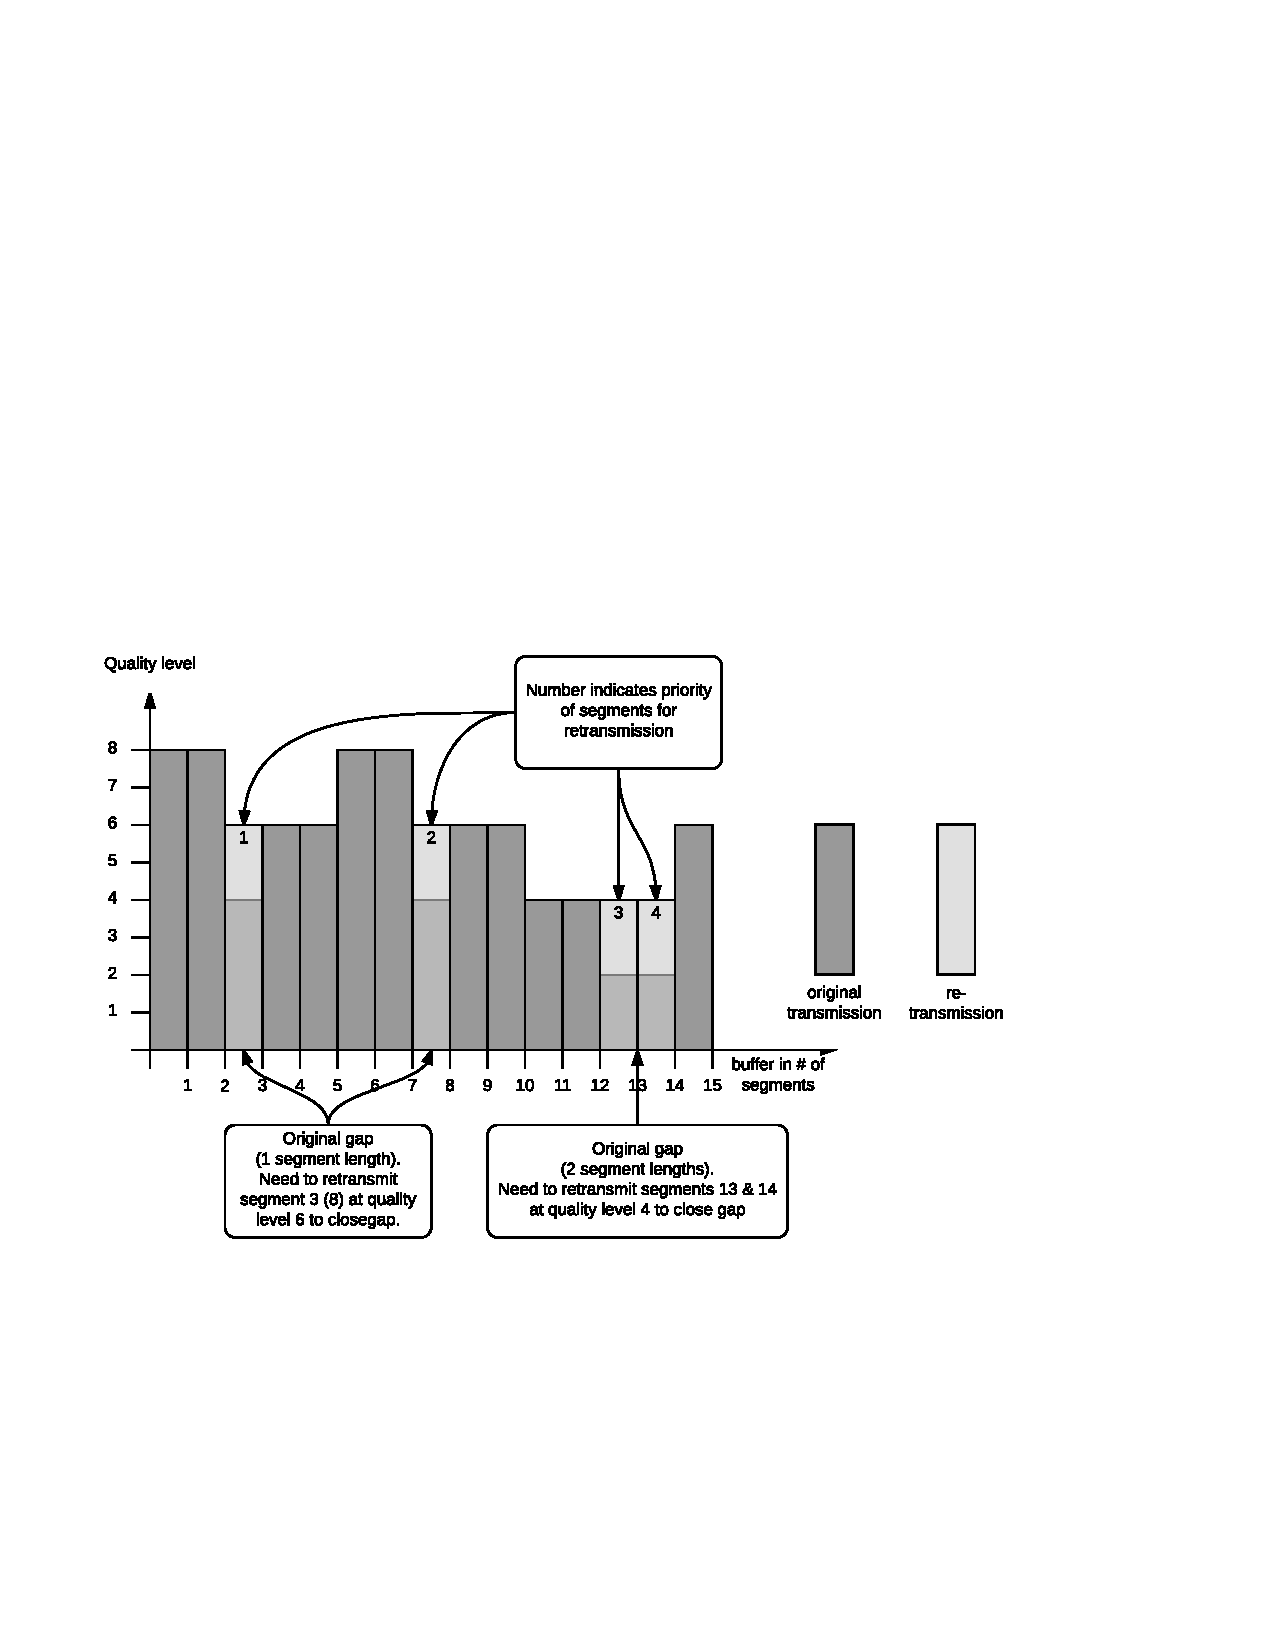
\includegraphics[width=.9\linewidth] {figures/Retrans_example.pdf}
% 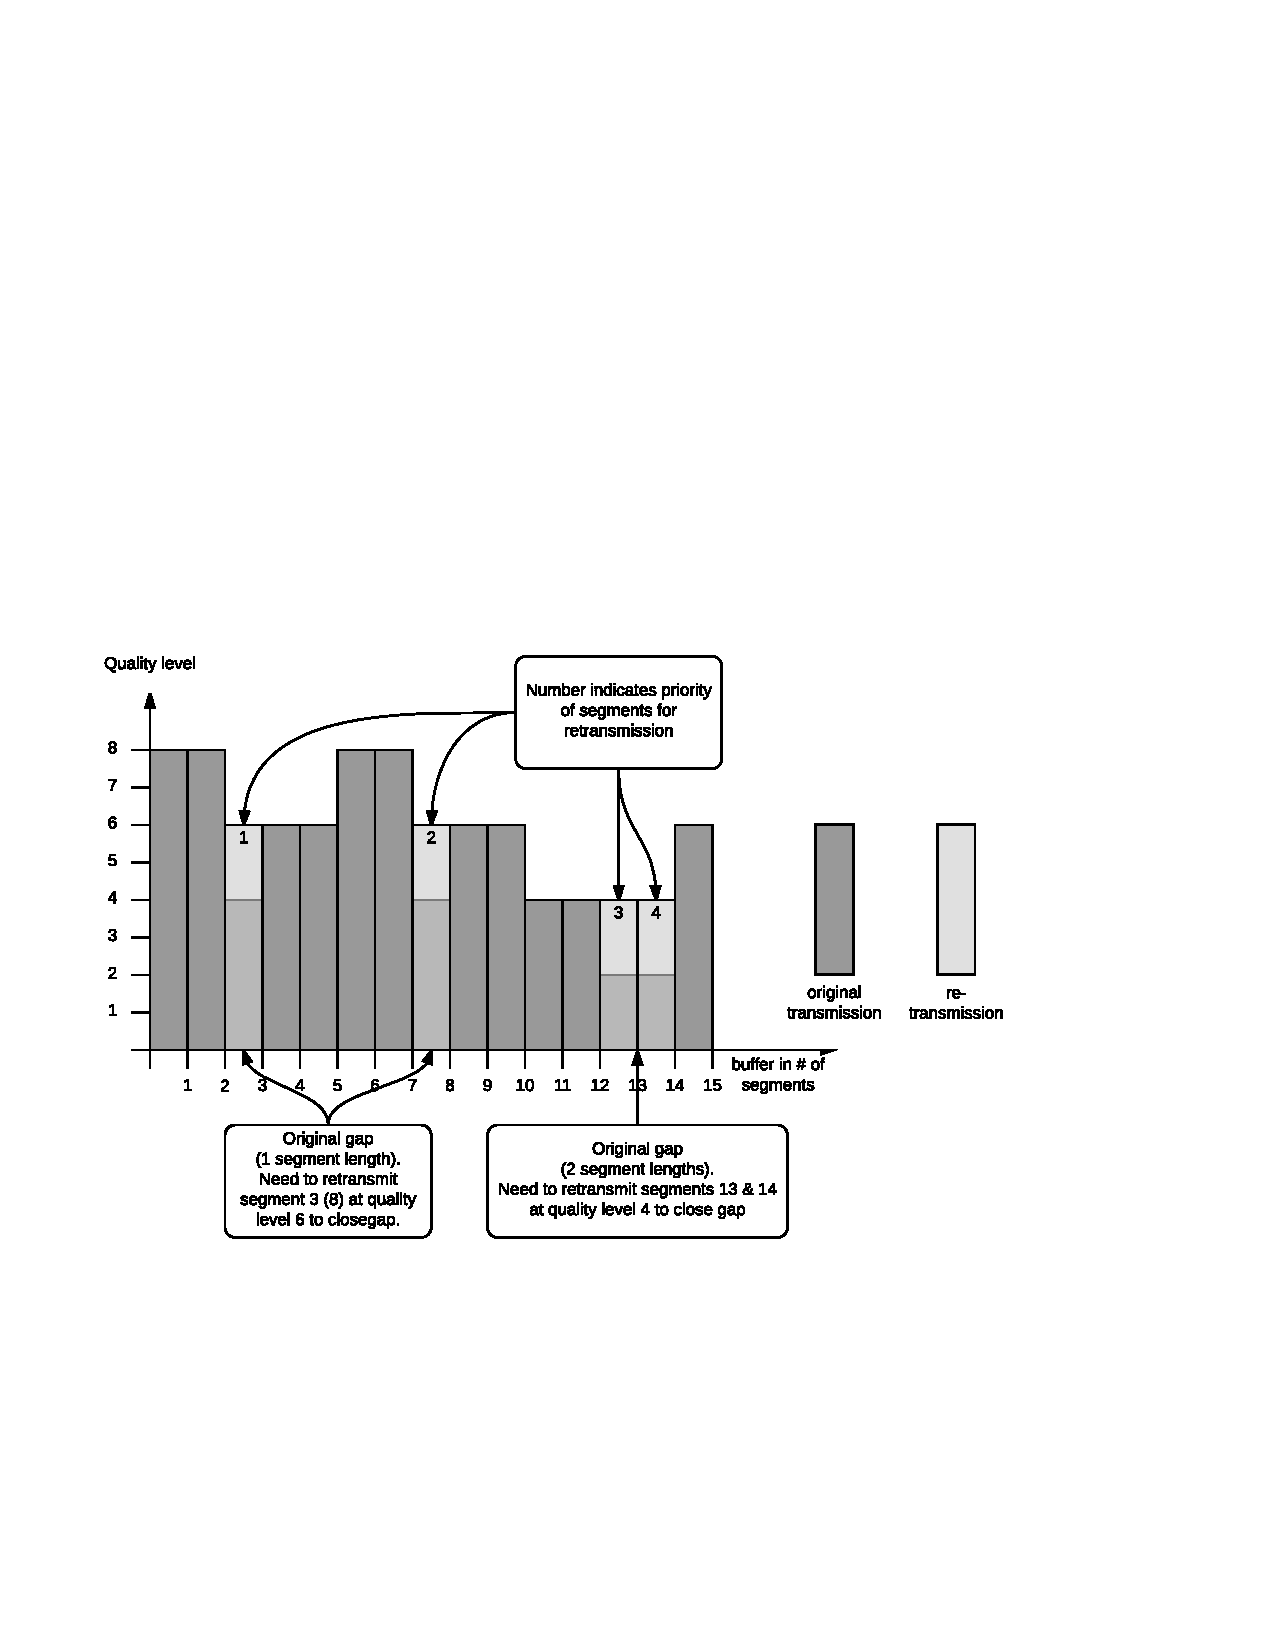
\includegraphics[scale=0.40, trim={0mm 100mm 0mm 90mm}] {figures/Retrans_example.pdf}
\caption{Example scenario for retransmissions. The QoE of this streaming session can be improved if, e.g., segments 3, 8, 13, and 14 are retransmitted in higher quality, assuming they arrive before their scheduled playout.}
\label{fig:retrans}
\vspace{-8pt}
\end{figure}

SQUAD's current approach is based on HTTP/1.1, which does not allow the parallel transmission of original segments and the retransmission of segments in a better quality. HTTP/2 over TCP allows this parallel transmission but does not prevent HOL blocking to efficiently perform retransmissions. In contrast, HTTP/2 over QUIC does not suffer from such inefficiencies and gives the application maximum control of individual streams and we show how this can be used to improve the QoE of ABR streaming.
\subsection{Analysis of Gaps in Streaming Sessions}
\label{subsec:ana_gap}
Akamai~\cite{AkamaiNetworkSIGOPS} is the world's largest CDN provider that delivers 15\%--30\% of global Internet traffic. Its CDN contains over 150,000 edge servers distributed in 90+ countries and 1200 ISPs around the world. To motivate the retransmission of segments as described in Sect.~\ref{subsec:retrans_sched}, we analyze an anonymized trace collected from Akamai's video CDN. This trace contains video streaming session information for a 3-day period in June 2014. The ABR streaming traffic in this trace contains 5 million video sessions originating from over 200,000 unique clients who were served by 1294 edge servers around the world. For each streaming session, each individual segment request is logged, which allows us to reconstruct the quality of the segments received at the client. Fig.~\ref{fig:gap_example} gives an example for one such streaming session we randomly picked for better illustration. As shown in Fig.~\ref{fig:gap_example}, this streaming session resulted in a  series of gaps. These gaps are potential candidates for segment retransmission that could lead to less quality level changes and, thus, an improve QoE. In Fig.~\ref{fig:gap_example}, we indicate that a retransmission of the segments in the later part of the stream could significantly impact the QoE.

\begin{figure}
\centering
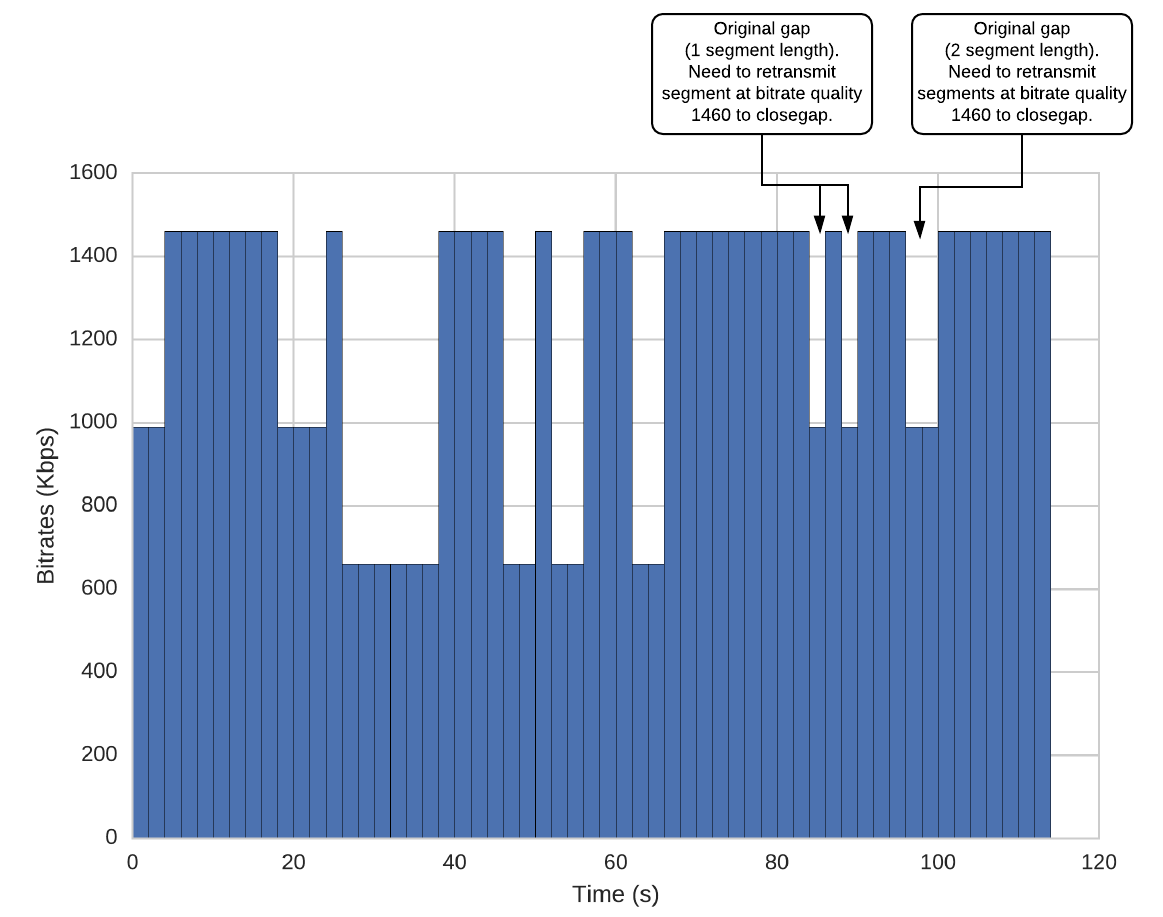
\includegraphics[width=.9\linewidth] {figures/mobonerun.png}
% 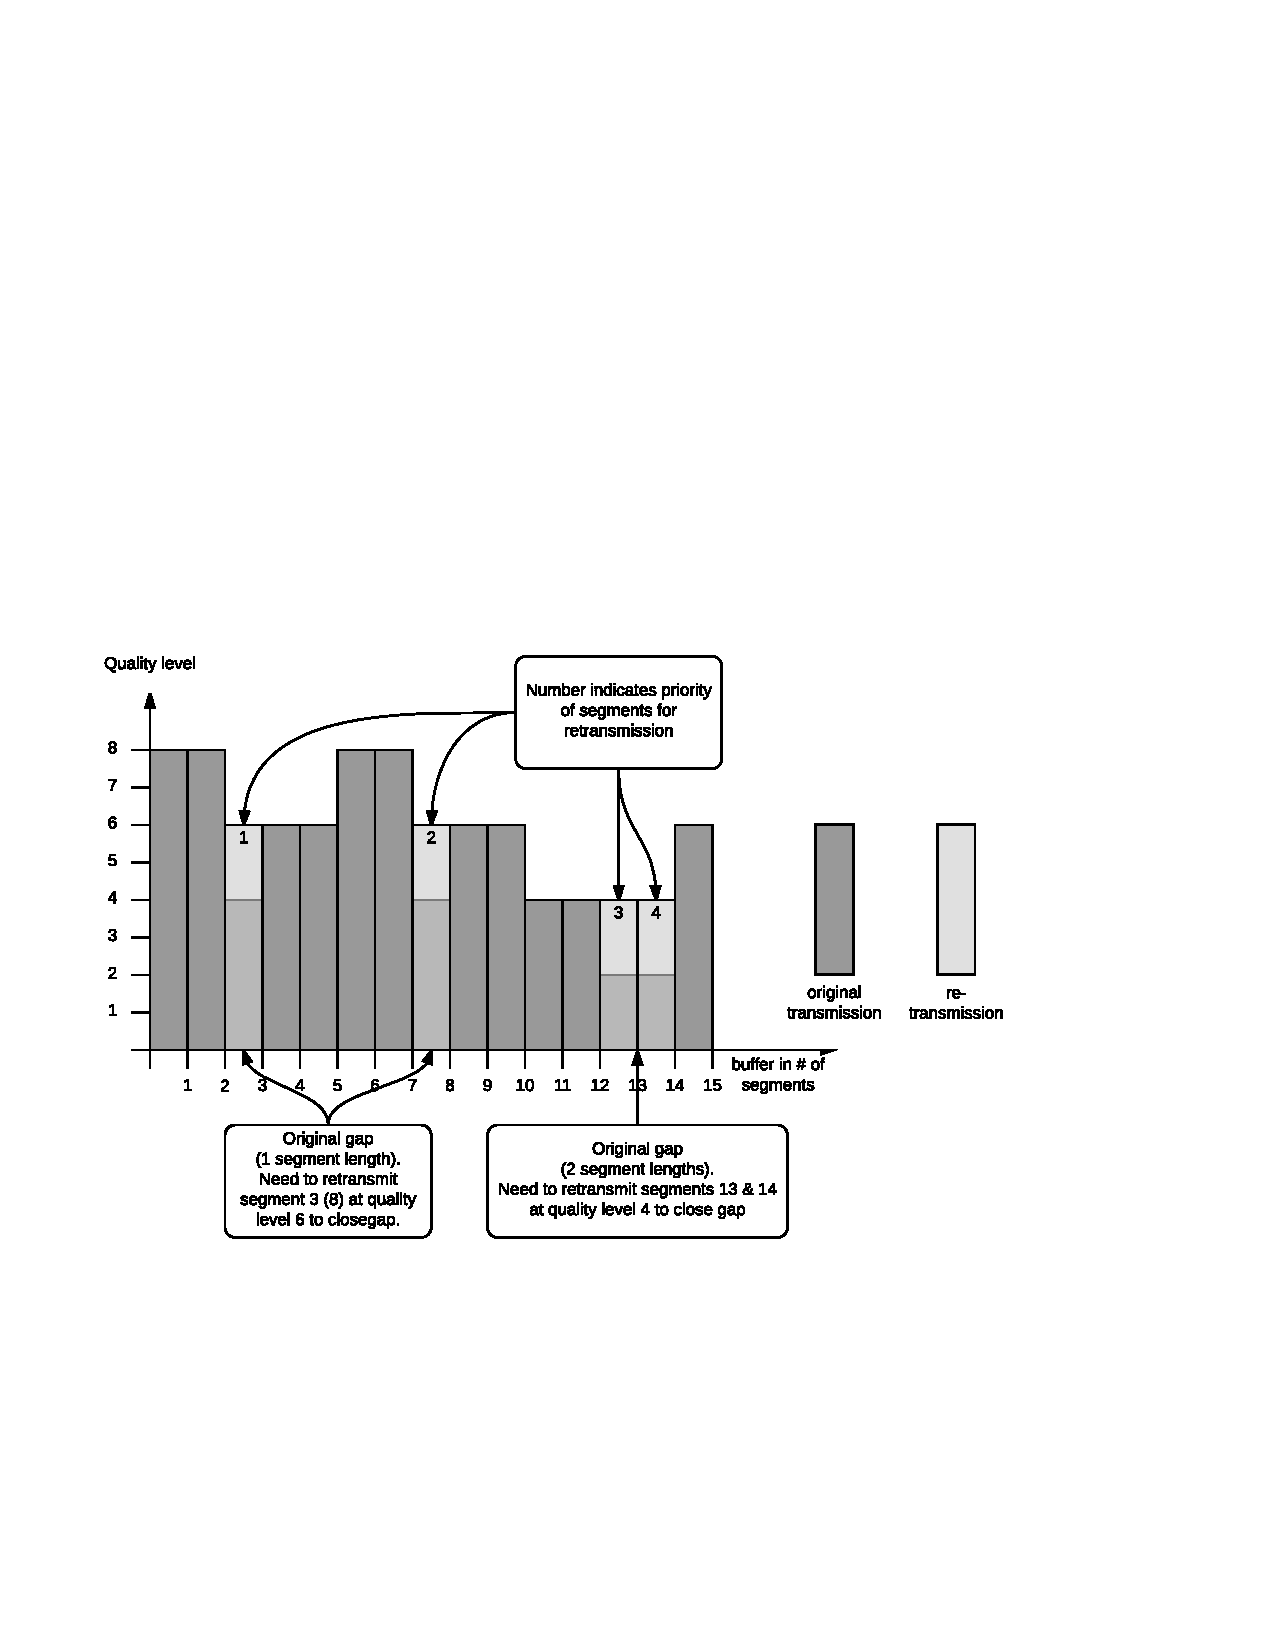
\includegraphics[scale=0.40, trim={0mm 100mm 0mm 90mm}] {figures/Retrans_example.pdf}
\caption{Original transmission of video stream from one randomly selected trace in the Akamai data set. The QoE of this video can be improved if the highlighted segments are retransmitted in higher quality, assuming they arrive before scheduled playout.}
\label{fig:gap_example}
\vspace{-18pt}
\end{figure}

In Fig.~\ref{fig:gap_cdf}, we show the results of our analysis for the complete data set which has approx. 5 million sessions, and for the a subset that only includes sessions for mobile devices, which has approx. 0.1 million sessions. This figure shows the percentage of sessions that have one or more gaps. Considering all sessions in the data set, 36.19\% of the sessions have at least one gap. These sessions could benefit from our segment retransmission approach. We also analyzed how many of the sessions with mobile clients have at least one gap. As shown in Fig.~\ref{fig:gap_cdf}, with 51.24\% this ratio is even higher. Obviously, this increase in sessions with at least one gap is not too surprising since mobile/wireless clients are assumed to experience higher bandwidth fluctuations than stationary/wired clients.

\begin{figure}
\centering
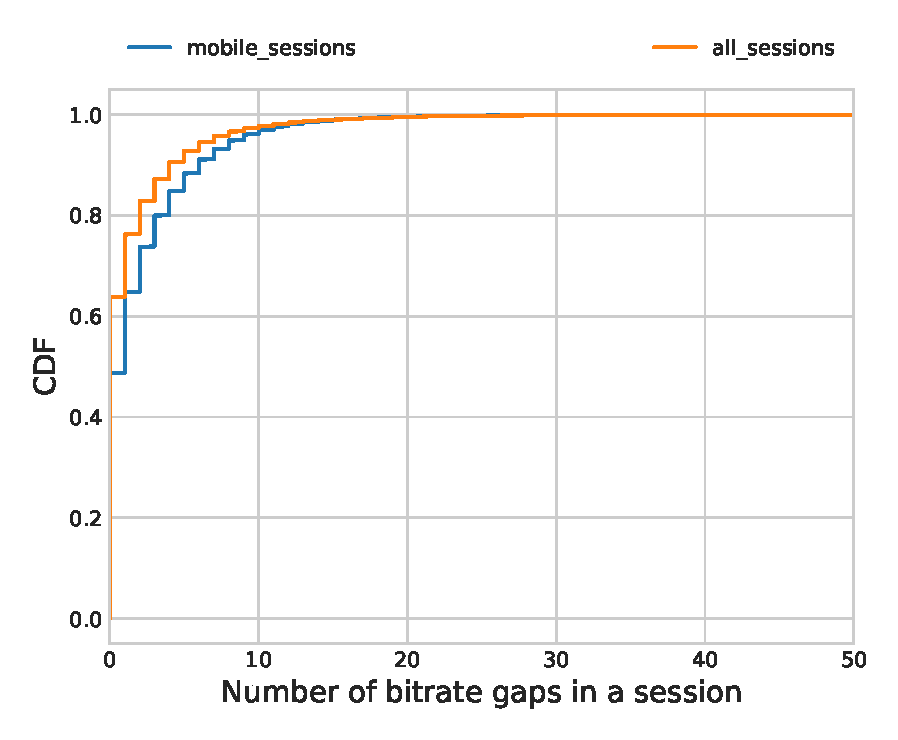
\includegraphics[width=.9\linewidth] {figures/all_gapCDF.eps}
% 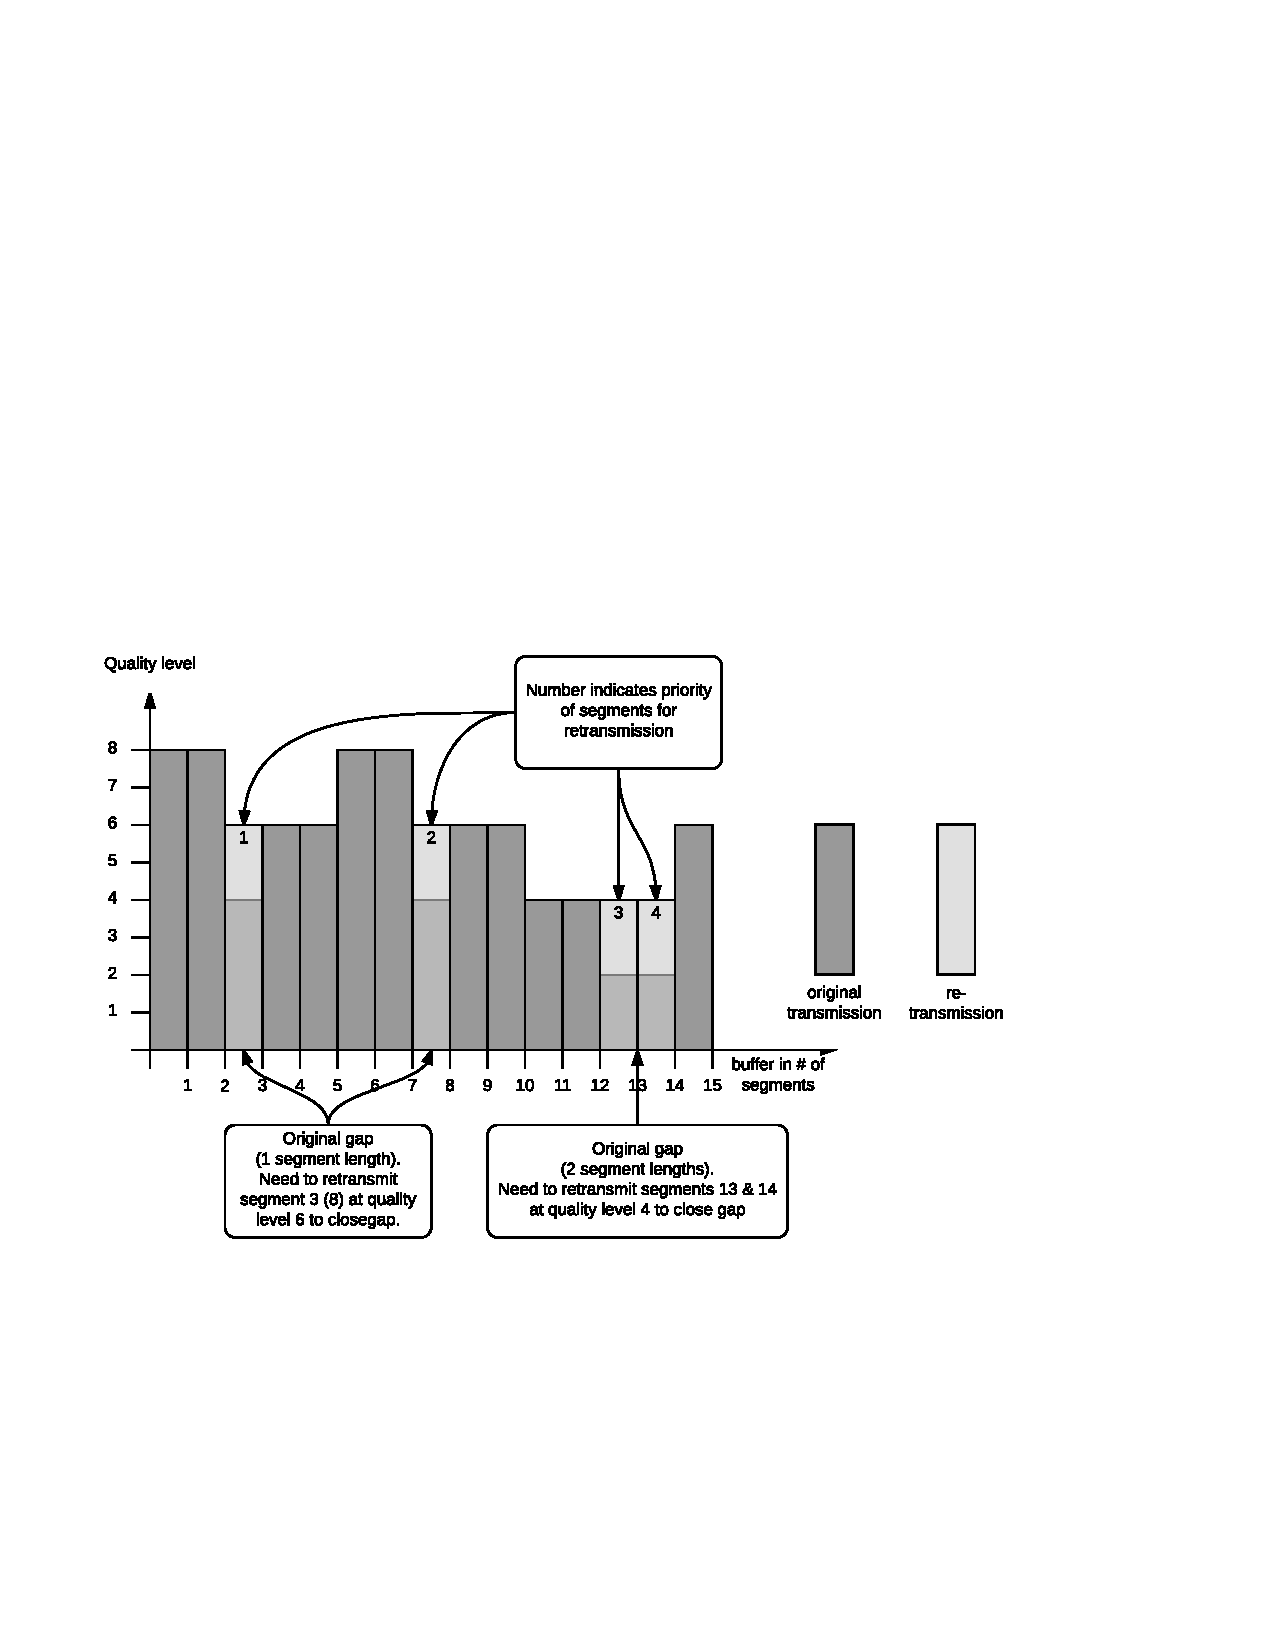
\includegraphics[scale=0.40, trim={0mm 100mm 0mm 90mm}] {figures/Retrans_example.pdf}
\caption{CDF for the number of sessions with one or more gaps for all sessions (orange) and mobile sessions (blue)}
\label{fig:gap_cdf}
\vspace{-12pt}
\end{figure}
\section{Segment retransmisson over HTTP/2}
\label{sec:retrans}

After introducing the basics of segment retransmission for ABR streaming and outlining its drawbacks in the case of HTTP/1.1 in Sect.~\ref{subsec:retrans_sched}, we introduce the usage of this approach in the case of HTTP/2 in this section. We first give an overview on the advantages and disadvantages of using our retransmission approach in the case of HTTP/2 over TCP and QUIC, respectively. This is followed by a description of the implementation of our approach. Results from an evaluation of this approach are presented in Sect.~\ref{sec:eval}.

\subsection{Example}
\label{subsec:example}
In the following, we compare a segment retransmission approach that is based on HTTP/2 over TCP (the current standard) with one that is based on HTTP/2 over QUIC. The TCP-based approach is shown in Fig.~\ref{fig:retr_tcp}. Here, we show a specific scenario of retransmissions for ABR streaming. In this scenario, HTTP/2 over TCP allows the multiplexing of multiple requests within a single TCP connection. This feature makes this approach more efficient than our existing HTTP/1.1 solution, since original  segment transmissions and retransmission can be performed in parallel. (In the case of HTTP/1.1, segments can either only be transmitted sequentially or a new TCP connection has to be established for the retransmissions). Despite the support of multiplexing several requests over a single TCP connection, this approach has several drawbacks. First of all, HOL blocking can lead to stalling. Such a case is indicated in Fig.~\ref{fig:retr_tcp}, where the first retransmitted TCP segment is lost. All of the following (original and retransmitted) TCP segments will be blocked from delivery to the application layer until the lost TCP segment is successfully received. This HOL blocking, caused by a TCP segment retransmission, prevents original segments from being delivered to the buffer of the video player. 
This can result in an incorrect estimate of the segment download rate and consequently an unnecessary reduction in bit rate quality for the download of future original segments. In the worst case, this causes the drainage of the video player buffer, which in turn will stall the video playout.

In contrast, an HTTP/2 over QUIC approach is not impacted by HOL blocking. Fig.~\ref{fig:retr_quic}, shows the same segment transmission scenario as in Fig.~\ref{fig:retr_tcp}. As opposed to the scenario shown in Fig.~\ref{fig:retr_tcp}, the QUIC-based approach does not prevent the original datagrams from being delivered to the video player buffer if the first retransmitted UDP datagram is lost. This should lead to a significant reduction in the risk of stalling and misinterpretation of the download rate. In addition, the application can decide if the lost retransmitted UDP datagram should be retrieved again or not. 
This decision can be based on buffer fill level, position of the retransmitted segment in the buffer, and observed download rate. With the use of QUIC, the application can also determine at which rate segments should be downloaded. For example, pacing~\cite{quic_pacing} can be applied for the retransmission of segments to assure that such transmissions only minimally interfere with the transmission of original segments.

\begin{figure*}[htb]
  \centering     
  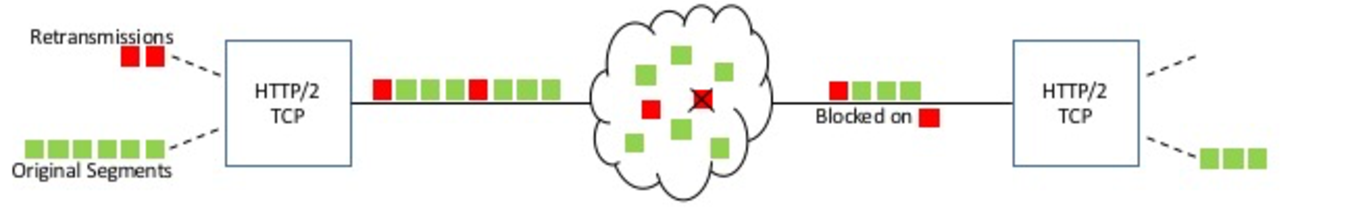
\includegraphics[width=.9\textwidth]{figures/retr_tcp.pdf}
  \centering
  \caption{This figure shows a scenario of original and retransmitted segment transmission in the case of HTTP/2 over TCP. The first of the retransmitted TCP segments (red) is lost, which leads to HOL blocking at the receiver.}
  \label{fig:retr_tcp}
  \vspace{-15pt}
\end {figure*}

\begin{figure*}[htb]
  \centering
  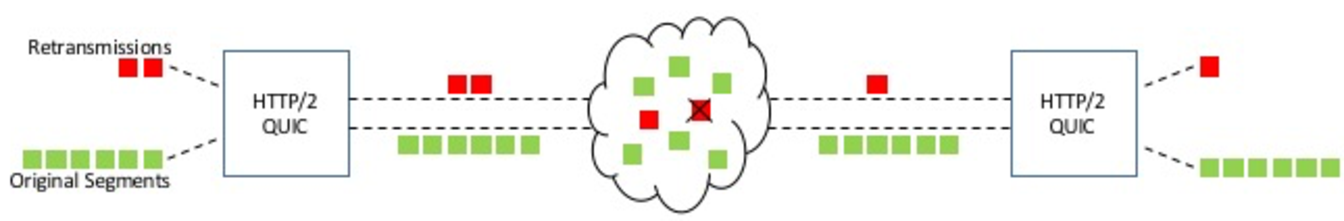
\includegraphics[width=.9\textwidth]{figures/retr_quic.pdf}
  \caption{This figure shows a scenario of original and retransmitted segment transmission in the case of HTTP/2 over QUIC. In contrast to Fig.~\ref{fig:retr_tcp}, the loss of a retransmitted UDP datagram (red) does not lead to HOL blocking and all original segments are delivered to the video player buffer.}
  \label{fig:retr_quic}
\end {figure*}

\subsection{Implementation}
\label{subsec:impl}
In this section, we give an overview of our implementation of ABR streaming that is based on HTTP/2 over QUIC that enables retransmissions of segments that have originally been transmitted in a low(er) quality (see Sect.~\ref{subsec:retrans_sched}).

\subsubsection{SQUAD with HTTP/2 and HTTP/1.1}
Since the multiplexing feature of HTTP/2 is unavailable in its predecessor, HTTP/1.1, the original version of SQUAD implements retransmission scheduling as a series of GET requests where at any given time there is only one outstanding request to the ABR streaming server. Intuitively, such a sequential implementation stalls the application pipeline and can lead to either conservative retransmission scheduling or a severe buffer drain.
To prevent stalling in case of a severe drop in measured download rate, SQUAD implements retransmission abandonment, which cancels segment retransmission when we observe that the segment will not be downloaded on time.
Our HTTP/2 implementation converts this sequential behavior into a parallel, multiplexed session of two simultaneous GET requests, where, at any given time there are a maximum of two possible streams active within a single connection. SQUAD is implemented as part of an open-source Python-based DASH player emulator, \texttt{AStream}.\footnote{\url{https://github.com/pari685/AStream}} For ease of integration, we use the Python-based HTTP/2 library, \texttt{hyper}\footnote{\url{https://github.com/Lukasa/hyper}}, in order to implement two multiplexed GET requests for original and retransmission segment downloads. Additionally, we implement multithreading to allow transmissions on both HTTP/2 streams to proceed independently. We note that HTTP/2 still uses the same TCP connection which suffers from HOL blocking as explained in Sect.~\ref{subsec:example}. and therefore, we also implement a SQUAD over QUIC approach which is introduced next. In order to make a fair comparison, we also adapt the original implementation of SQUAD to use \texttt{hyper} for making HTTP/1.1 requests.

\subsubsection{SQUAD with QUIC}
Similar to the experiment above, we implement multiplexed sessions for original and retransmitted segment downloads using QUIC. However, we include the use of IPC message streams with minimal overhead to communicate between the QUIC client (implemented in C++) and the AStream player (implemented in Python). Unlike HTTP/2 over TCP, QUIC does not suffer from HOL blocking and is designed to deliver data to the application as soon as they arrive at the receiver and a stream within a QUIC connection is not adversely affected by events that cause delay or loss of packets on a parallel, ongoing stream. At the time of this implementation, we used Chromium for Linux with QUIC version \texttt{Q043}. In order to provide support for multiplexed streams for SQUAD, we perform the following modifications on the \texttt{QUIC client}\footnote{\url{https://www.chromium.org/quic/playing-with-quic}} code provided by Google: (i) we create and synchronize simultaneous streams within a single connection, (ii) we introduce IPC messaging not only to send commands between AStream and QUIC but also to provide intermediate chunk download rate measurements to the SQUAD ABR algorithm.

We note that this work does not focus on modifying SQUAD to perform optimally with a protocol such as QUIC but is instead intended as a study to evaluate  the performance of SQUAD retransmissions over QUIC in order to determine if QoE can be improved with such an approach.
\section{Evaluation Design}
\label{sec:eval}
In this section, we describe a series of experiments, which are specifically designed to study the QoE performance of using QUIC and HTTP/2 for ABR video streaming with a focus on segment retransmission. We compare the results of these experiments  with the baseline approach that uses HTTP/1.1. The server nodes (denoted as \textit{Server1 - Server4} in Fig. \ref{fig:clab_topo}) run a Caddy server (version=0.10.10) \cite{caddy} with the experimental QUIC mode enabled such that the clients can stream DASH videos either over TCP or QUIC. We chose the Caddy server as it is a production server which is capable of simultaneously supporting QUIC, HTTP1.1, and HTTP/2 over TCP with TLS1.2. All experiments use an excerpt of the \texttt{BigBuckBunny} dataset \cite{lederer2012dynamic} (unless stated otherwise) that comprises a 300s-long video with a 2s segment duration and the corresponding MPD file. We extended the MPD file by providing the size of each segment in each of the available quality levels.\footnote{We use segment sizes in the MPD file since this was introduced in AStreamer. This can easily be replaced by using byte ranges, which are available in real-world, ABR streaming solutions.} The quality bitrates available in this MPD file are the following: $\{${0.09, 0.13, 0.18, 0.22, 0.26, 0.33, 0.59, 0.79, 1.03, 1.24, 1.54, 2.48, 3.52, 4.21}$\}$Mbps. The client nodes run the SQUAD ABR algorithm~\cite{Wang:TOMM:2017} described above, which is implemented in a Python-based DASH player~\cite{parikshit:icc}.

\begin{figure}
\centering
% \includegraphics[scale=0.40, trim={0mm 120mm 0mm 20mm}]
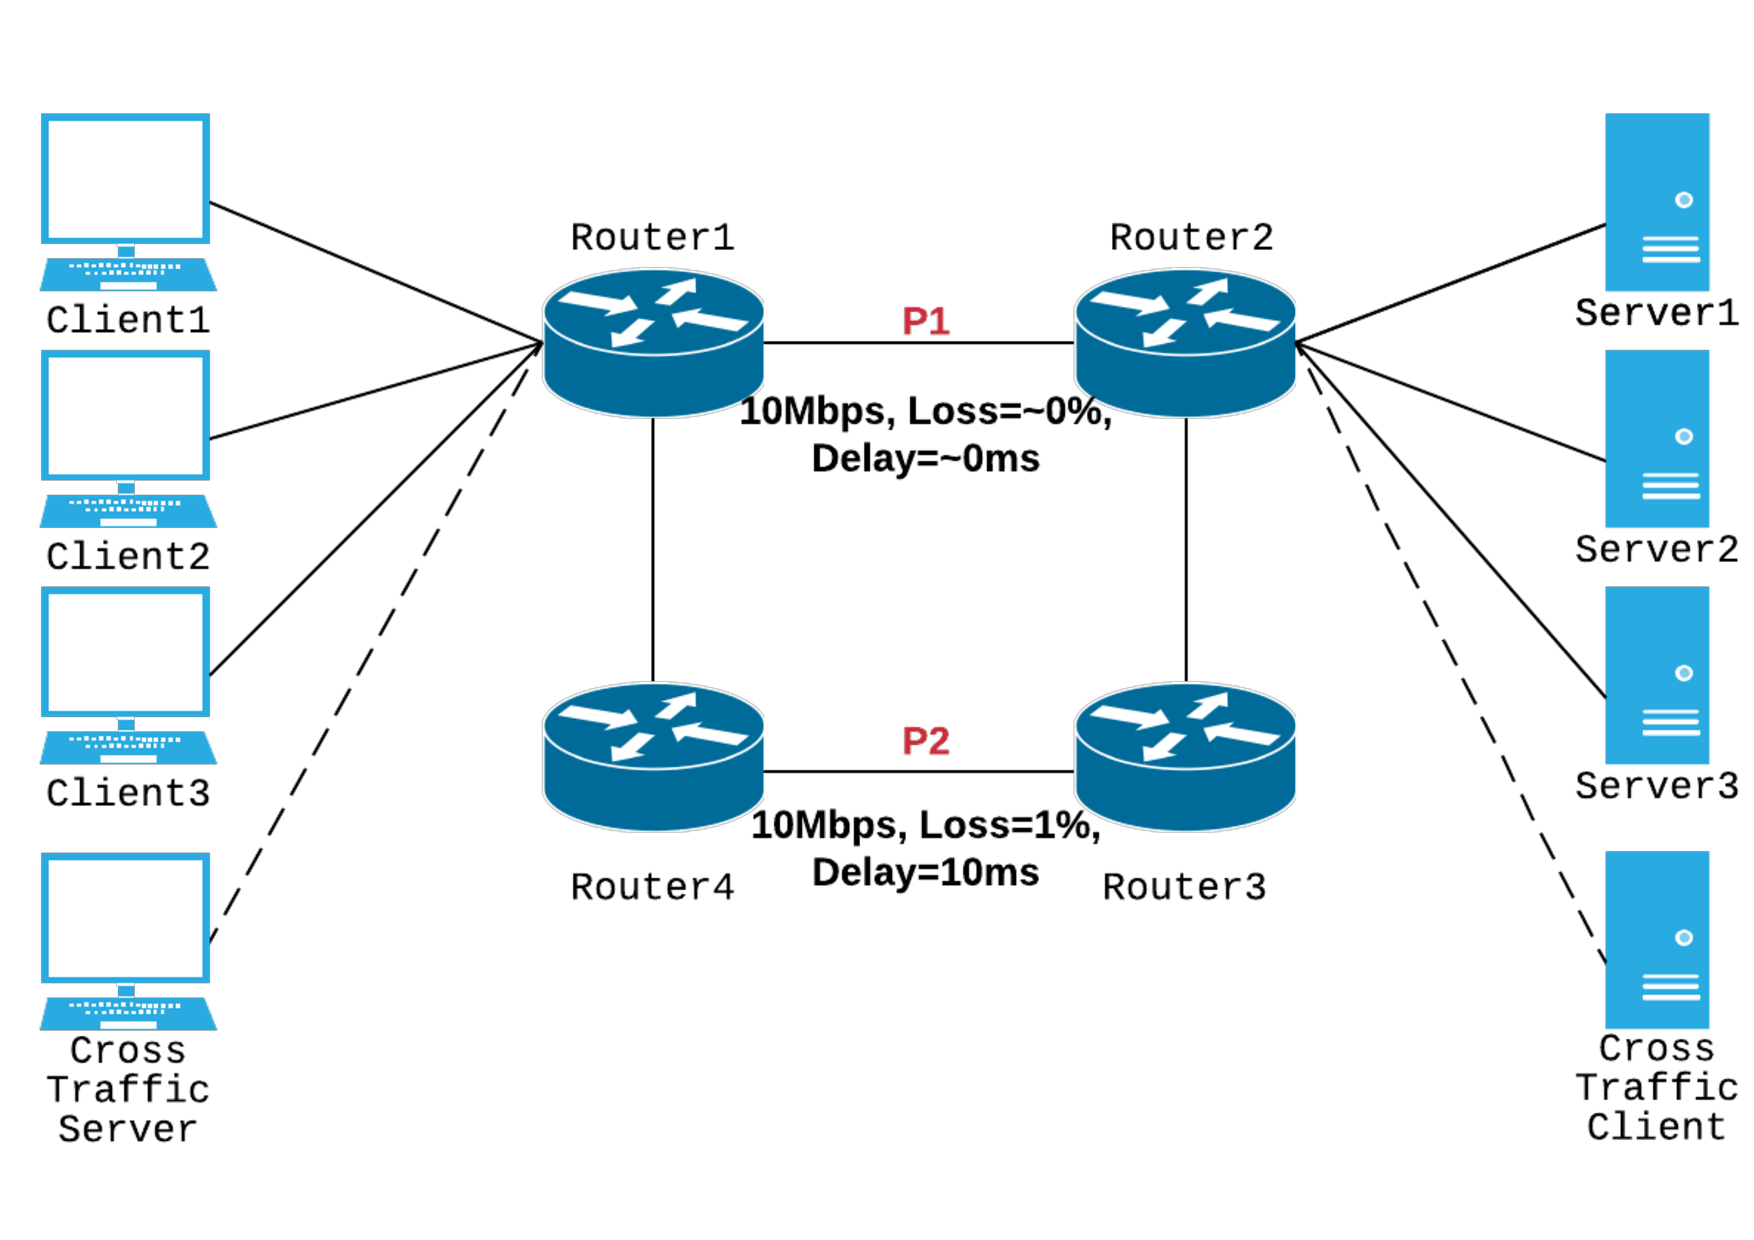
\includegraphics[width=\linewidth,angle=0,scale=0.85, trim={2cm 2cm 2cm 2cm}]{figures/ACM_MM18_topo_v2.pdf}
\caption{Cloudlab topology used for controlled experiments}
\label{fig:clab_topo}
\vspace{-20pt}
\end{figure}

\label{sec:eval}
\begin{comment}
\subsection{Segment Download Time}
As stated in previous work~\cite{Wang:TOMM:2017}{}, the SQUAD algorithm uses the following two equations in order to reliably estimate if the retransmission of a segment can be successfully performed before its playout deadline. 
\DB{Add Eq12 and Eq13 from TOMM paper - should I add these or is it unnecessary?}. Our first set of experiments compares the download times of varying segment sizes, which we believe will lend valuable insight to evaluate the ABR streaming experiments that follow. 
In order to utilize the benefit of the multiplexing feature of HTTP/2 and QUIC for SQUAD, we make slight modifications to the implementation without altering the details of the SQUAD algorithm itself.
\end{comment}
\subsection{Testbed}
For our controlled experiments, we use Cloudlab \cite{RicciEide} which is a geographically distributed testbed for
the development, deployment, and validation of cloud-based services. The CloudLab infrastructure consists of several different racks of varying compute and storage resources designed to provide isolated performance. The topology shown in Fig.~\ref{fig:clab_topo} consists of four clients and four servers connected by two paths \textbf{P1} and \textbf{P2} with the default set to \textbf{P1} unless stated otherwise. All nodes run vanilla Ubuntu 14.04 where all TCP related experiments use TCP Cubic. In order to account for statistical variance, every experiment in the controlled environment is repeated 30 times. For the single client experiments, we use \textit{Client1} and \textit{Server1} as the default pair and include other server and client pairs for parallel client cases.
\begin{figure*}[t!]
\centering
\begin{subfigure}[t]{0.33\textwidth}
   \captionsetup{justification=centering,margin=4.5cm}
    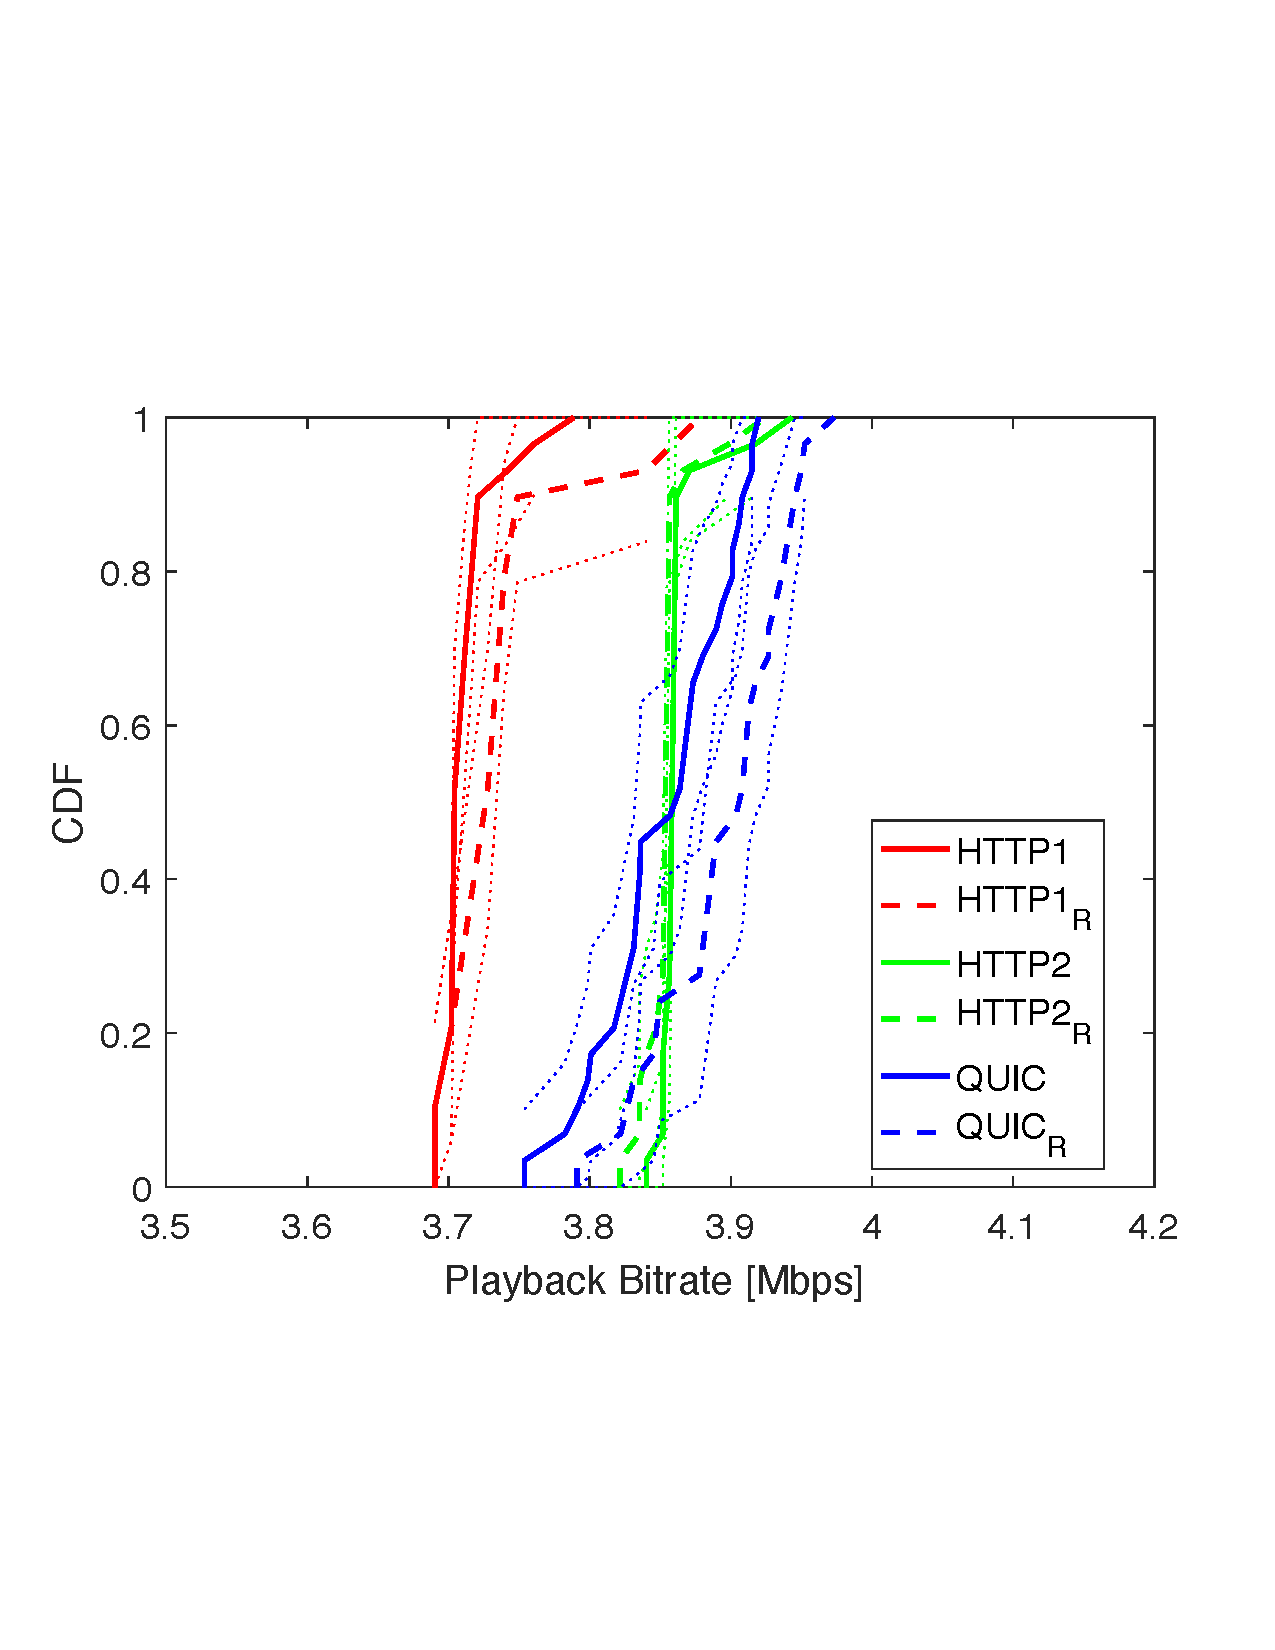
\includegraphics[trim={0 5cm 0 6cm}, scale=0.24]{figures/CDF_bitrat_squad_udpstair_nd18.pdf}
     \caption{}
    \label{fig:udpstairbitrate}
  \end{subfigure}
  \begin{subfigure}[t]{0.33\textwidth}
  \captionsetup{justification=raggedright,singlelinecheck=false,margin=2.5cm}
    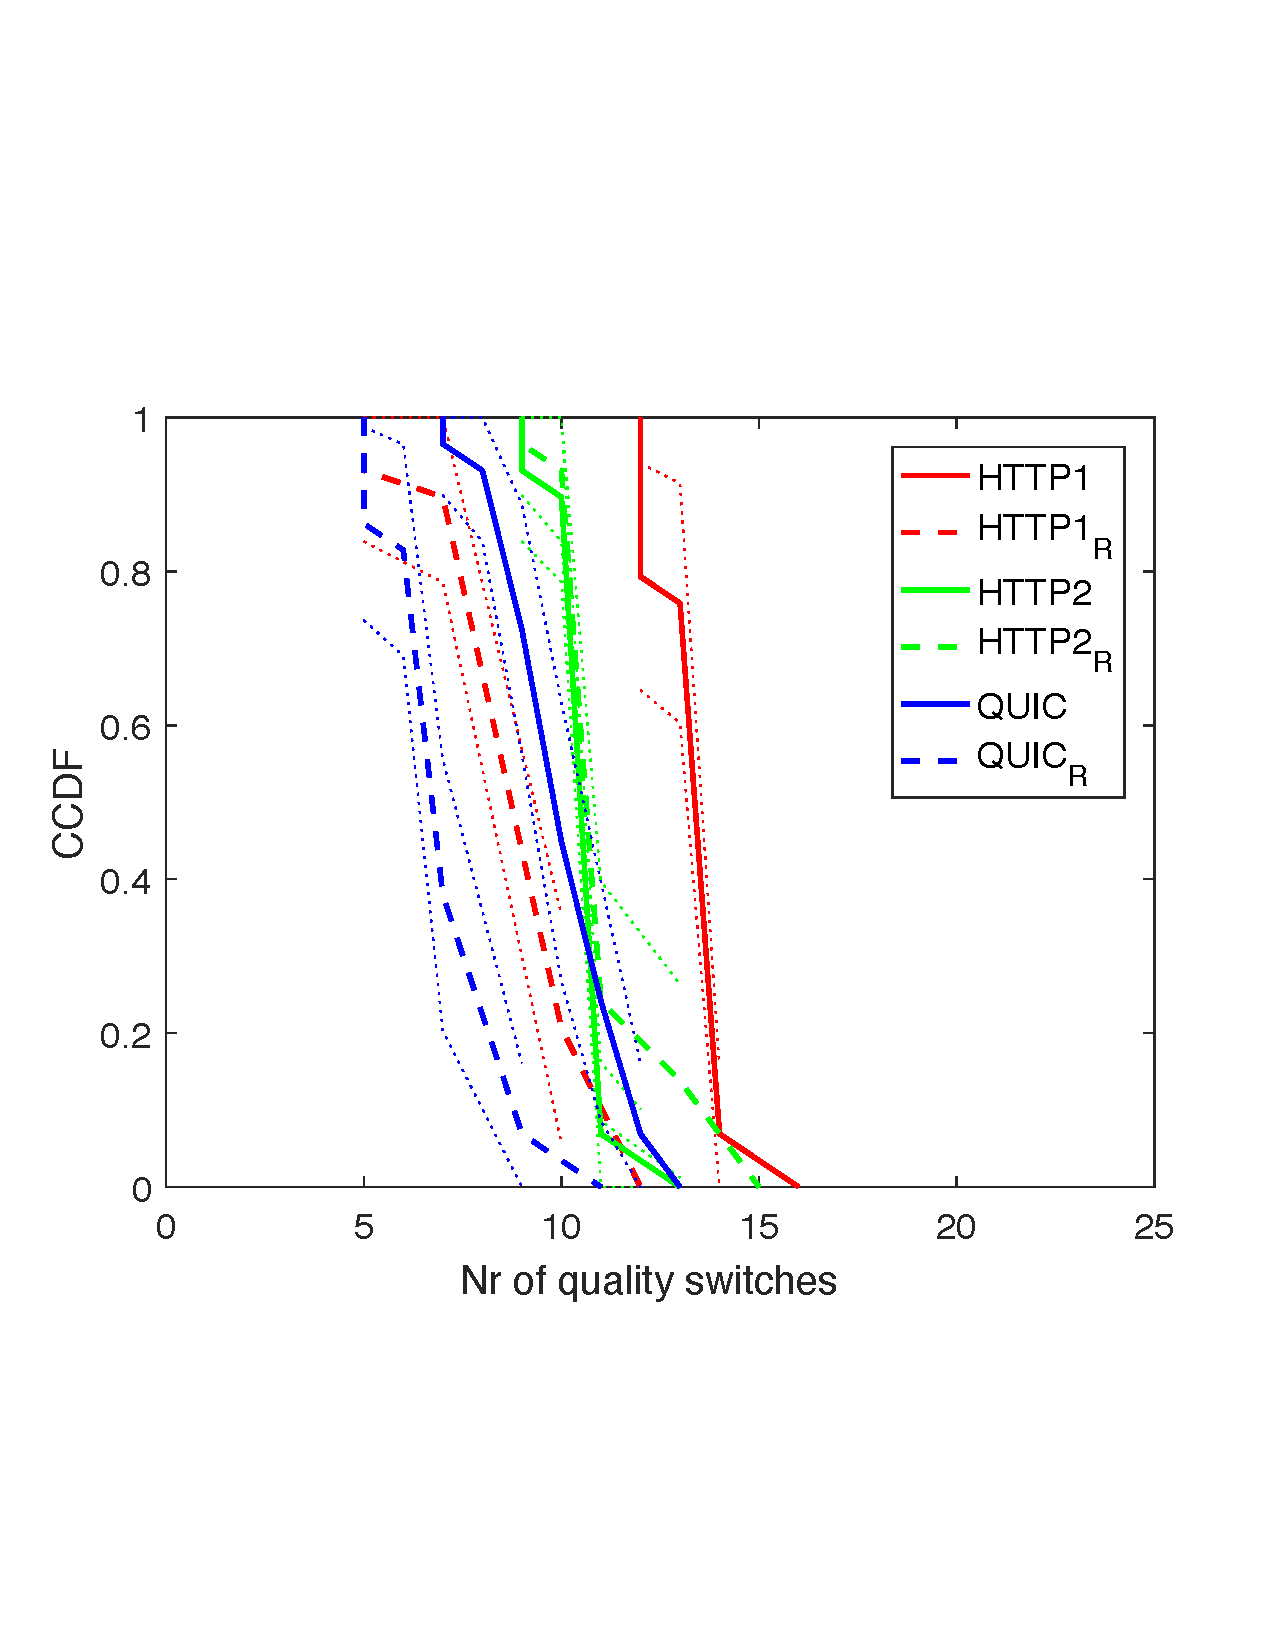
\includegraphics[trim={0 5cm 0 6cm}, scale=0.24]{figures/CDF_cntswitch_squad_udpstair_nd18.pdf}
    \caption{}
    \label{fig:udpstaircntsw}
  \end{subfigure}
  \begin{subfigure}[t]{0.33\textwidth}
  \captionsetup{justification=centering,margin=1.5cm}
    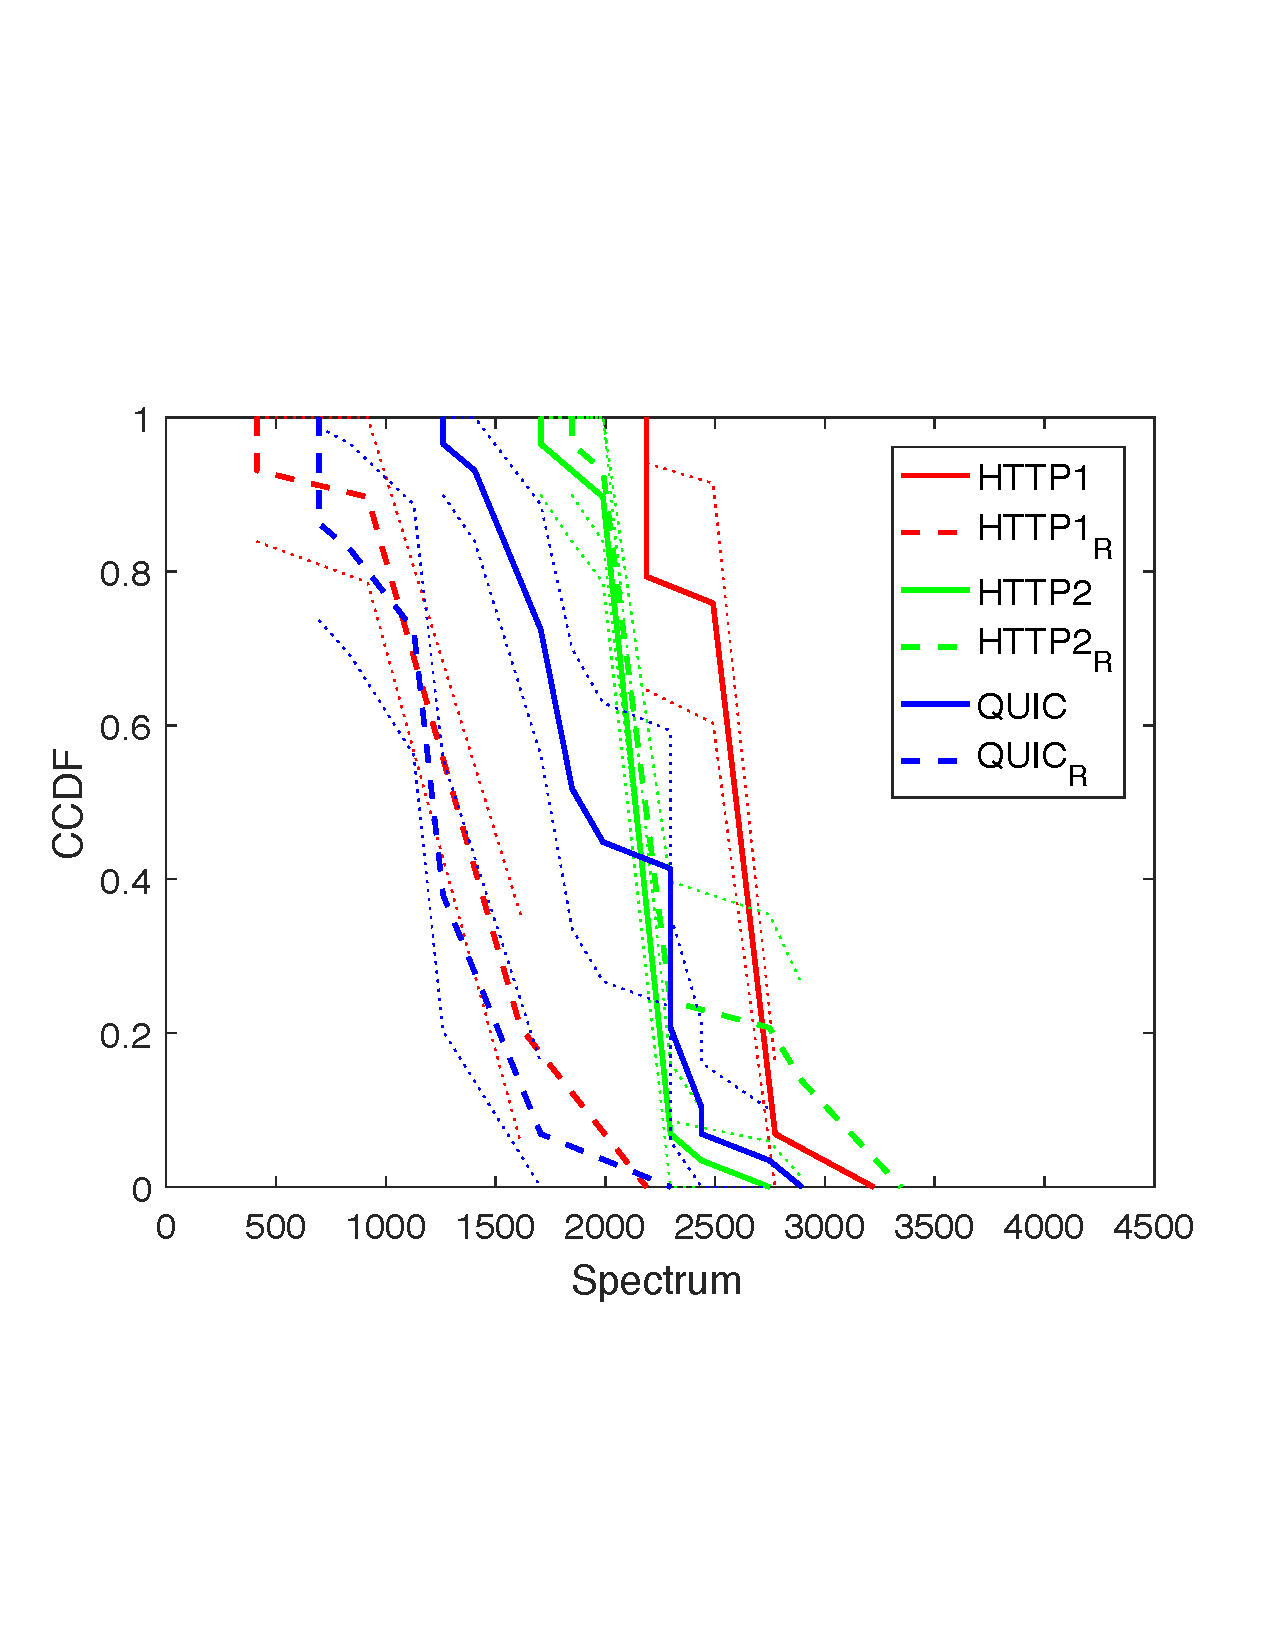
\includegraphics[trim={0 5cm 0 6cm}, scale=0.24]{figures/CDF_magswitch_squad_udpstair_nd18.pdf}
    \caption{}
    \label{fig:udpstairmagsw}
  \end{subfigure}
 \centering
   \vspace{-15pt}
  \caption{Single Client Measurements - Rate Limited with UDP-Staircase cross traffic. 
  %Here, we see results of using a stepwise UDP cross traffic increasing in increments of 3Mbps upto a maximum of 9Mbps where 
  QUIC has a significantly better overall Quality of Experience compared to HTTP/1.1 and HTTP/2, which is further improved by retransmissions. Note, subscript ``R'' denotes ABR segment retransmissions.}
  \label{fig:udpstair}
   \vspace{-10pt}
\end {figure*}
\subsubsection{Single Client: Rate Limiting with UDP}
\label{subsubsec:single_udp}
In order to systematically compare the performance of HTTP/1.1, HTTP/2 and QUIC in a controlled environment, we use the \texttt{Iperf}\footnote{\url{https://iperf.fr/iperf-doc.php}} application to generate competing UDP traffic (denoted cross traffic) of varying amplitudes. The first set of experiments consists of repeating a stepwise variation of cross traffic where the duration of each step is 11s and varies as follows: \{0-11s: 0Mbps, 12-23s: 3Mbps, 24-35s: 6Mbps, 36-55s: 9Mbps, 56-67s: 6Mbps, 68-79s: 3Mbps, 80-91s: 0Mbps\} (then the pattern repeats until t=300s). Fig. \ref{fig:udpstair} shows the CDF and CCDF along with 95\% confidence intervals for upper and lower bounds of the QoE metrics described at the beginning of this section. In Fig. \ref{fig:udpstairbitrate}, we observe that QUIC clients have the highest average quality bitrate or $AQB$ when compared to both HTTP/1.1 and HTTP/2. It is also worth noting that other QoE metrics such as number of quality changes ($\#QS$) and the Spectrum, $H$, are significantly improved with the use of QUIC retransmissions. Figure \ref{fig:udpw9} shows results for the "W" cross traffic case where we use the \texttt{Iperf} application to generate competing UDP cross traffic that creates a "W" shaped bottleneck bandwidth and varies as follows: \{0-20s: 9Mbps, 21-40s: 5Mbps, 41-60s: 9Mbps, 61-80s: 0Mbps\} (then the pattern repeats until t=300s). Although, in terms of $AQB$, $\#QS$ and $H$, HTTP/2 clients appear to experience the best QoE, we observed that the clients also experience a relatively high rebuffering ratio, $RB$, of 4\% while using HTTP/2 for ABR streaming. Since it is well known that the foremost objective of any ABR client streaming algorithm is to eliminate or reduce rebuffering, we conclude that QUIC, especially with the use of segment retransmissions, also performs significantly better than HTTP/1.1 and HTTP/2 for the "W" cross traffic case. 
\begin{figure*}[htb!]
\centering
\begin{subfigure}[t]{0.33\textwidth}
   \captionsetup{justification=centering,margin=4.5cm}
    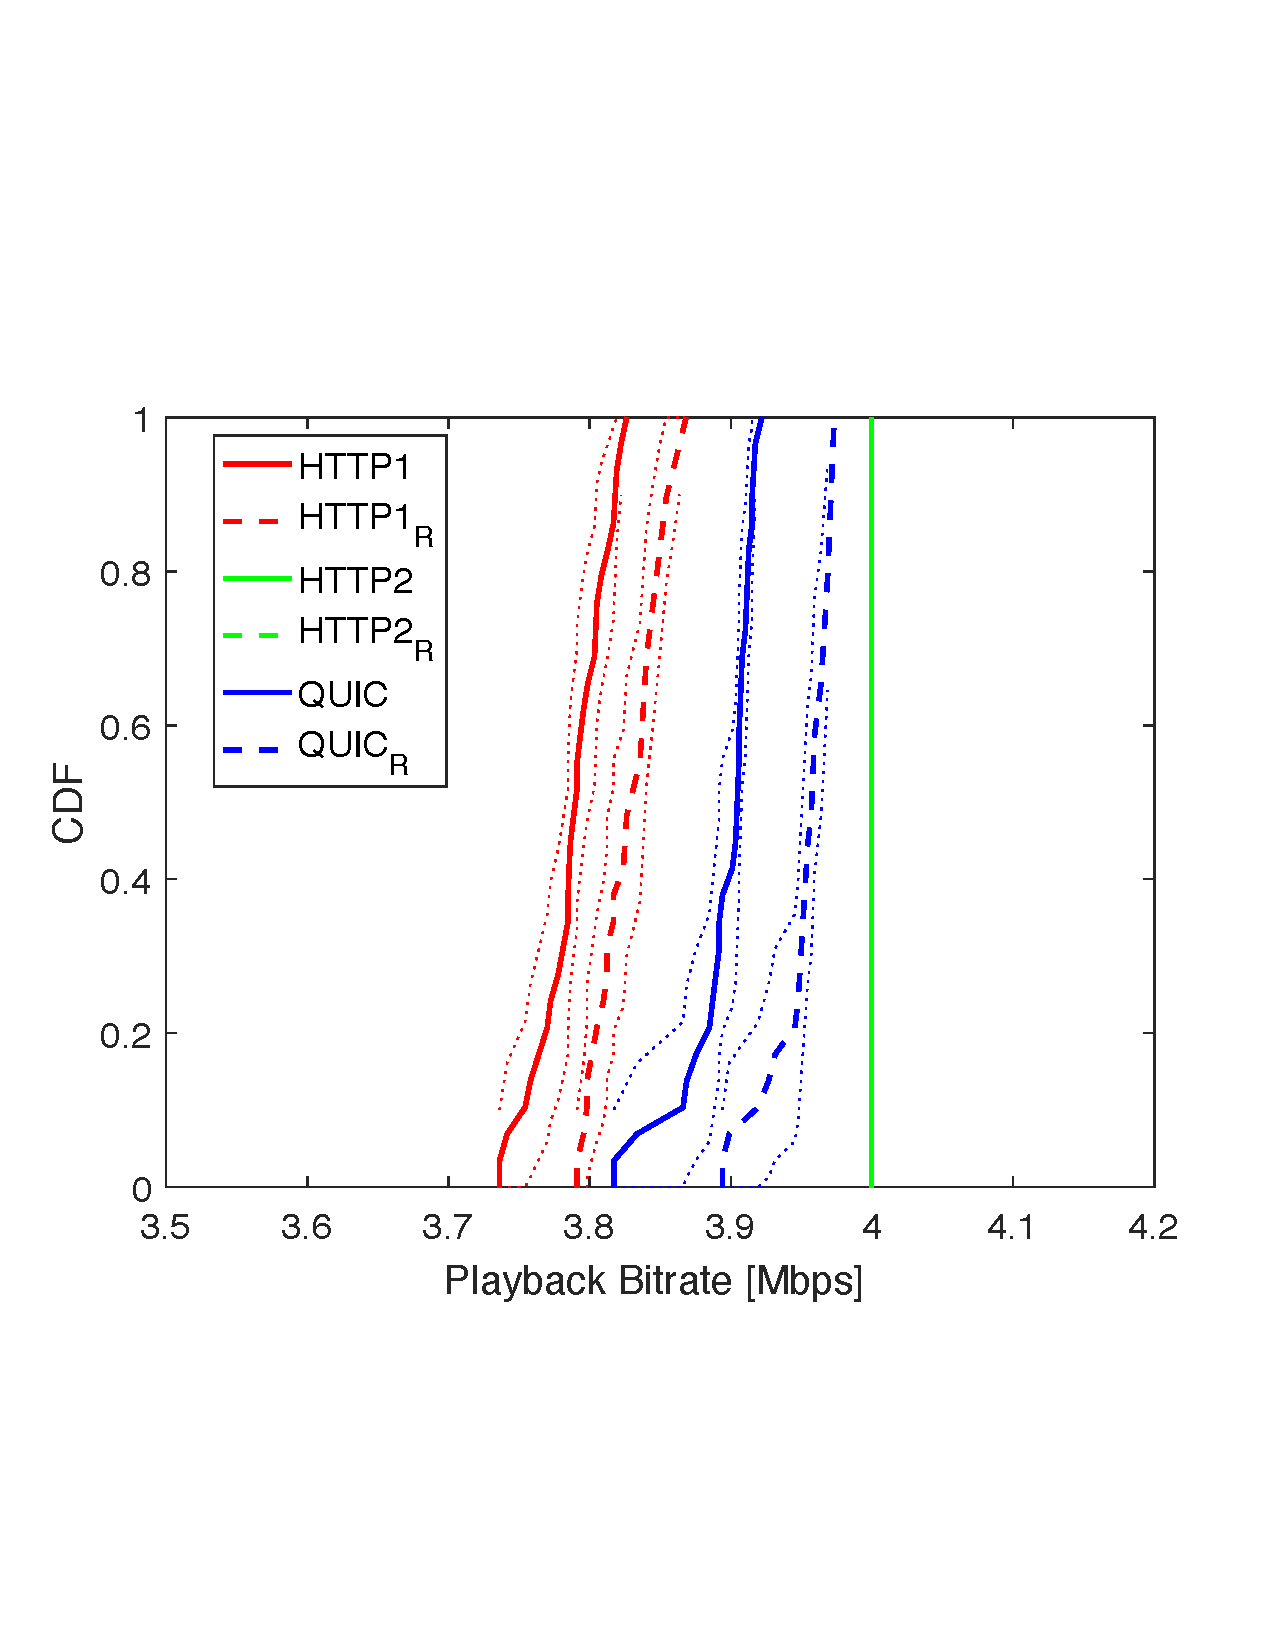
\includegraphics[trim={0 5cm 0 7cm}, scale=0.24]{figures/CDF_bitrat_squad_udpw9_nd18.pdf}
     \caption{}
    \label{fig:udpw9bitrate}
  \end{subfigure}
  \begin{subfigure}[t]{0.33\textwidth}
  \captionsetup{justification=raggedright,singlelinecheck=false,margin=2.5cm}
    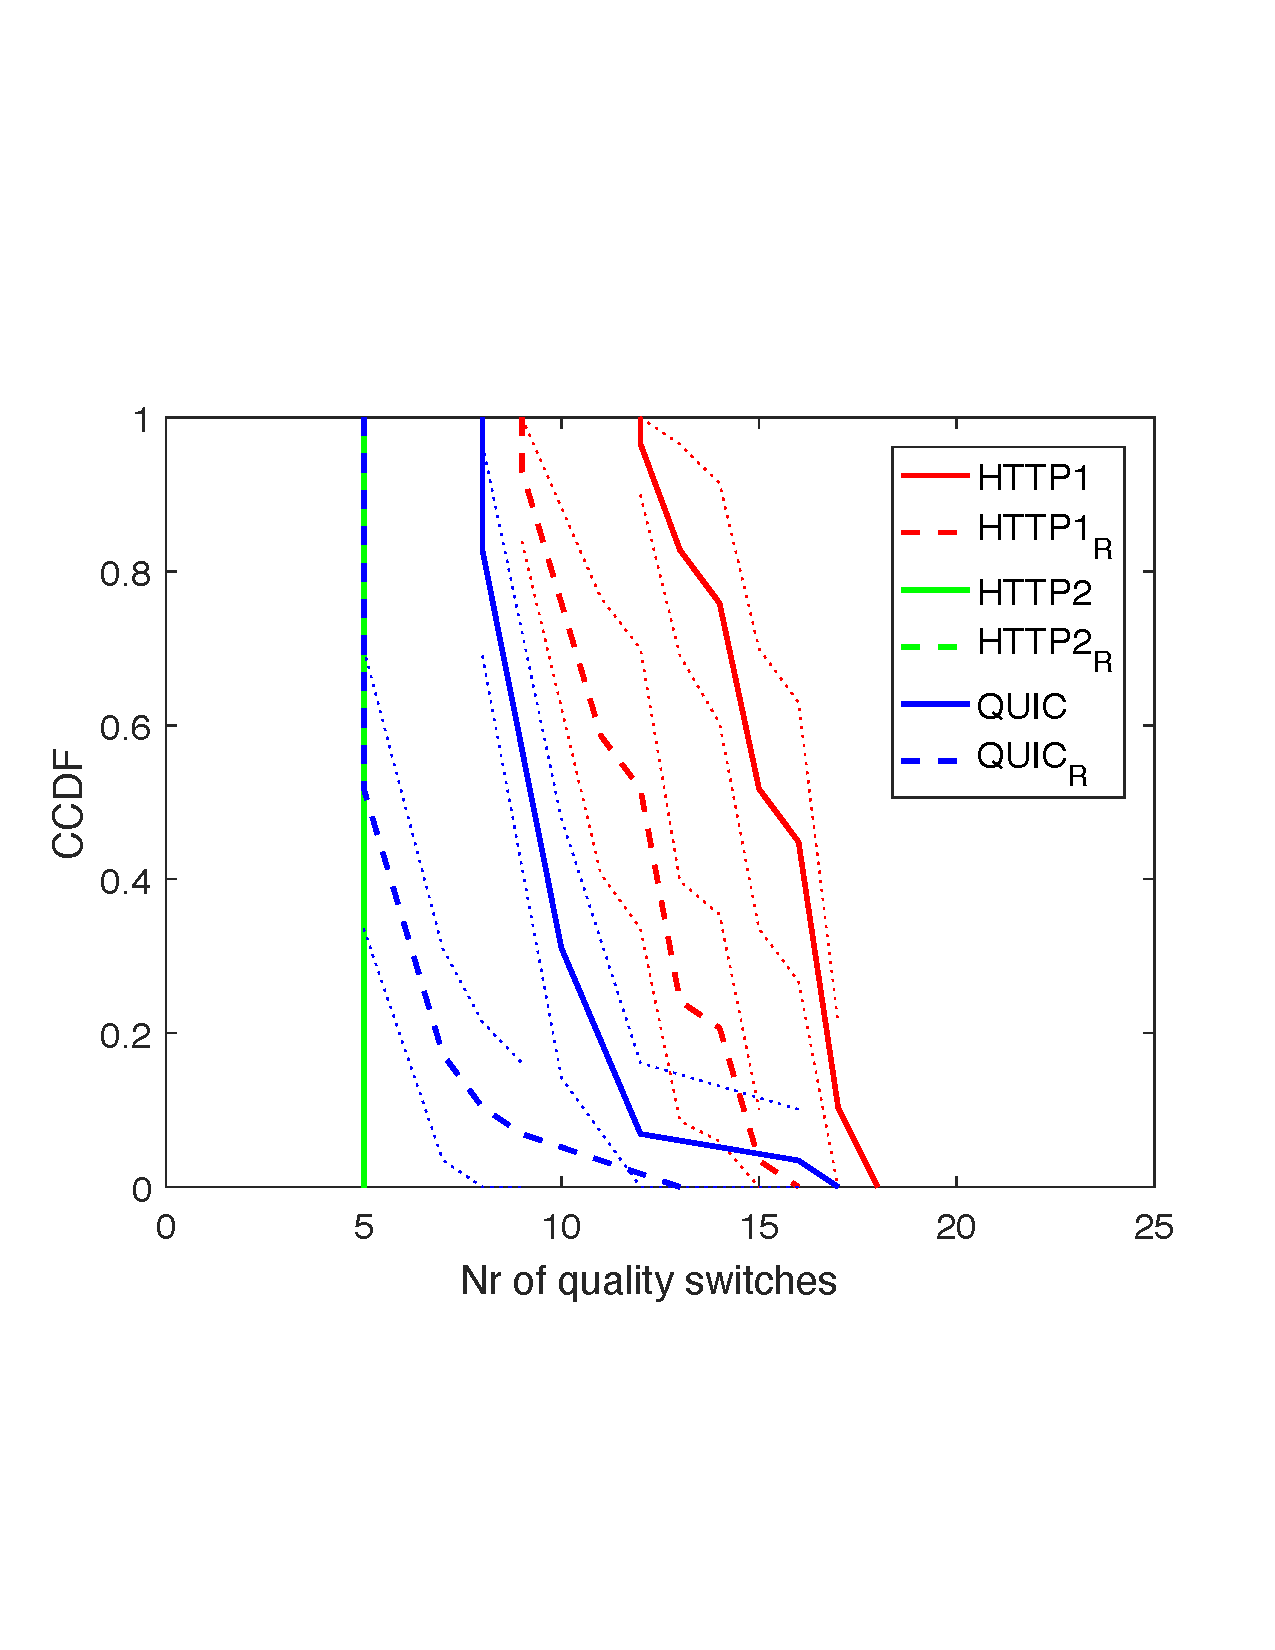
\includegraphics[trim={0 5cm 0 7cm}, scale=0.24]{figures/CDF_cntswitch_squad_udpw9_nd18.pdf}
    \caption{}
    \label{fig:udpw9cntsw}
  \end{subfigure}
  \begin{subfigure}[t]{0.33\textwidth}
  \captionsetup{justification=centering,margin=1.5cm}
    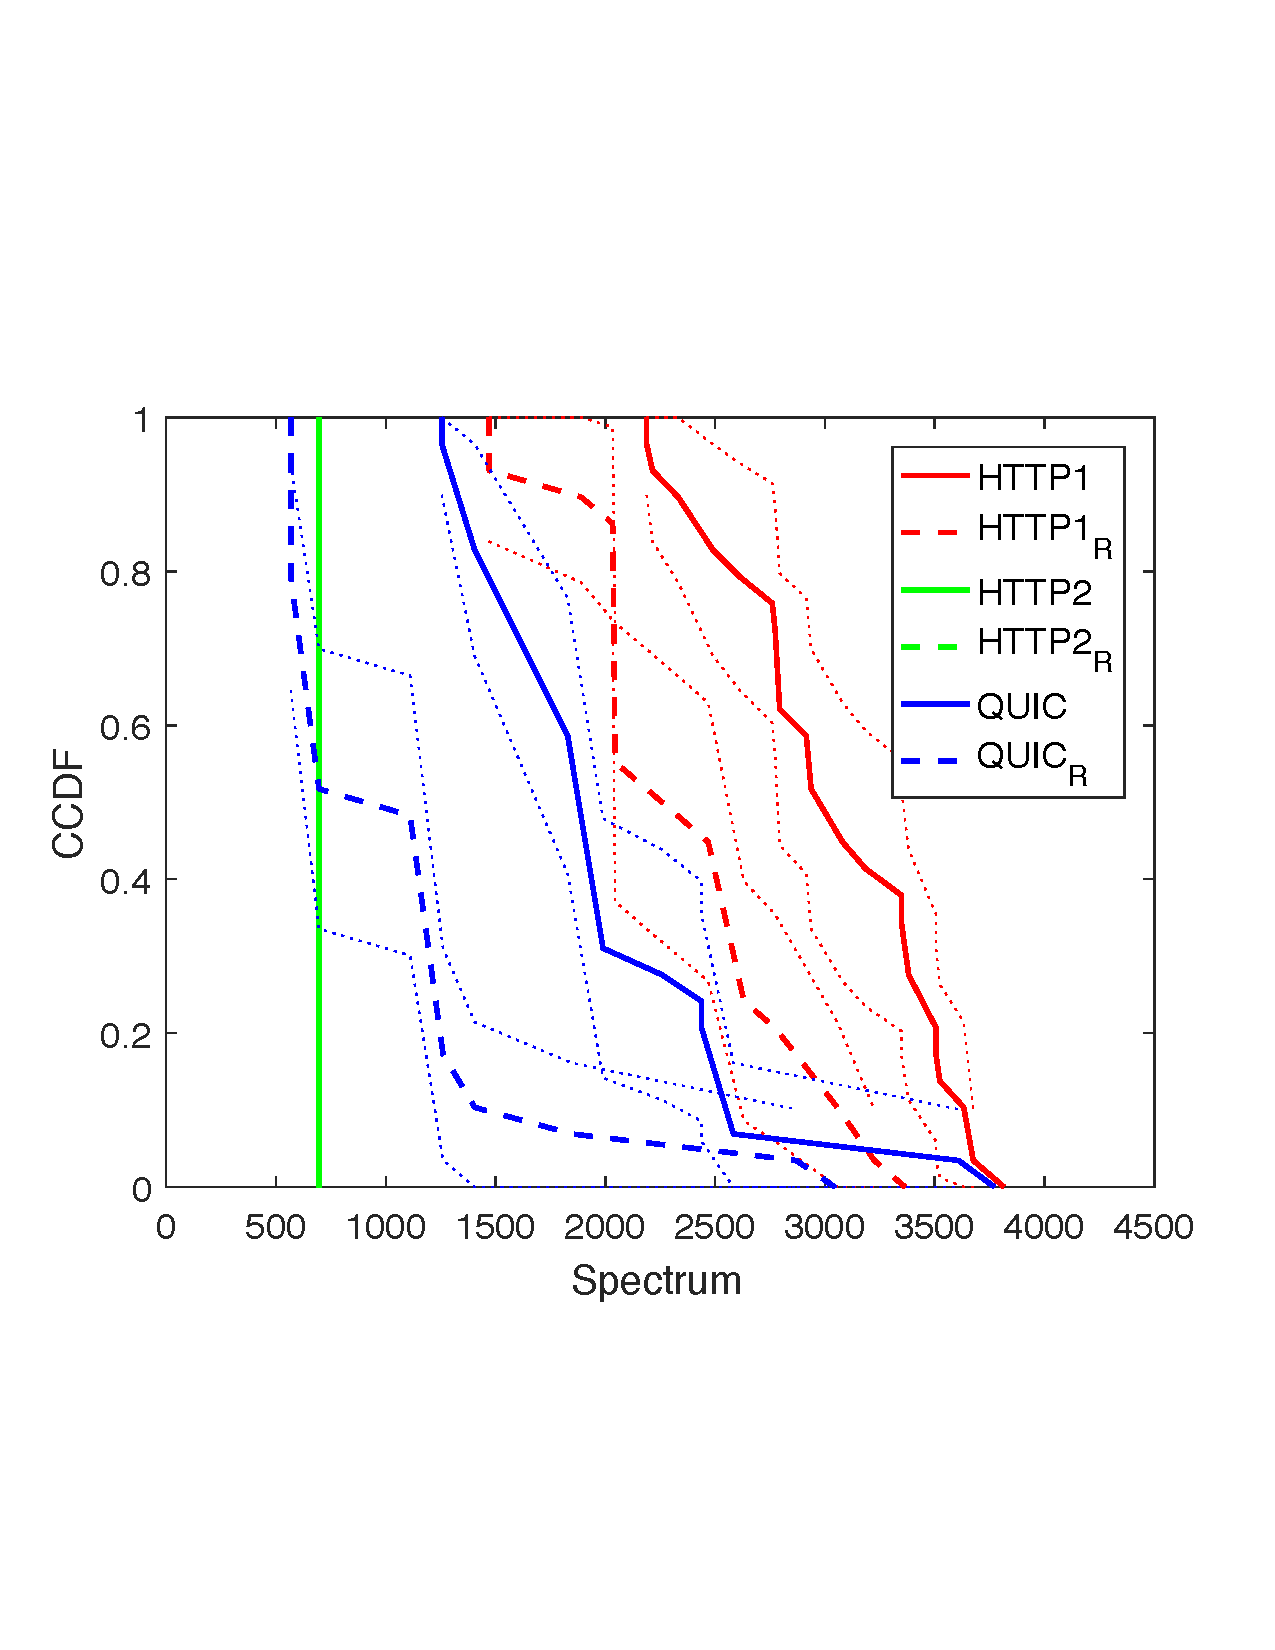
\includegraphics[trim={0 5cm 0 7cm}, scale=0.24]{figures/CDF_magswitch_squad_udpw9_nd18.pdf}
    \caption{}
    \label{fig:udpw9magsw}
  \end{subfigure}
 \centering
  \vspace{-12pt}
  \caption{Single Client Measurements - Rate Limited with UDP-W cross traffic. 
  % Here, we see results of using UDP with a "W" shaped bandwidth as cross traffic varying in amplitude between 9Mbps and 5Mbps. 
  QUIC has a significantly better overall QoE compared to HTTP/1.1. Although HTTP/2 sessions appear to be having a higher QoE, all clients experience 4\% rebuffering. Note, subscript ``R'' denotes ABR segment retransmissions.}
  \label{fig:udpw9}
   \vspace{-15pt}
\end {figure*}

\subsubsection{Single Client: Re-ordering and HOL}
\label{subsubsec:hol}
\begin{figure*}[htb!]
\centering
\begin{subfigure}[t]{0.33\textwidth}
   \captionsetup{justification=centering,margin=0.5cm}
    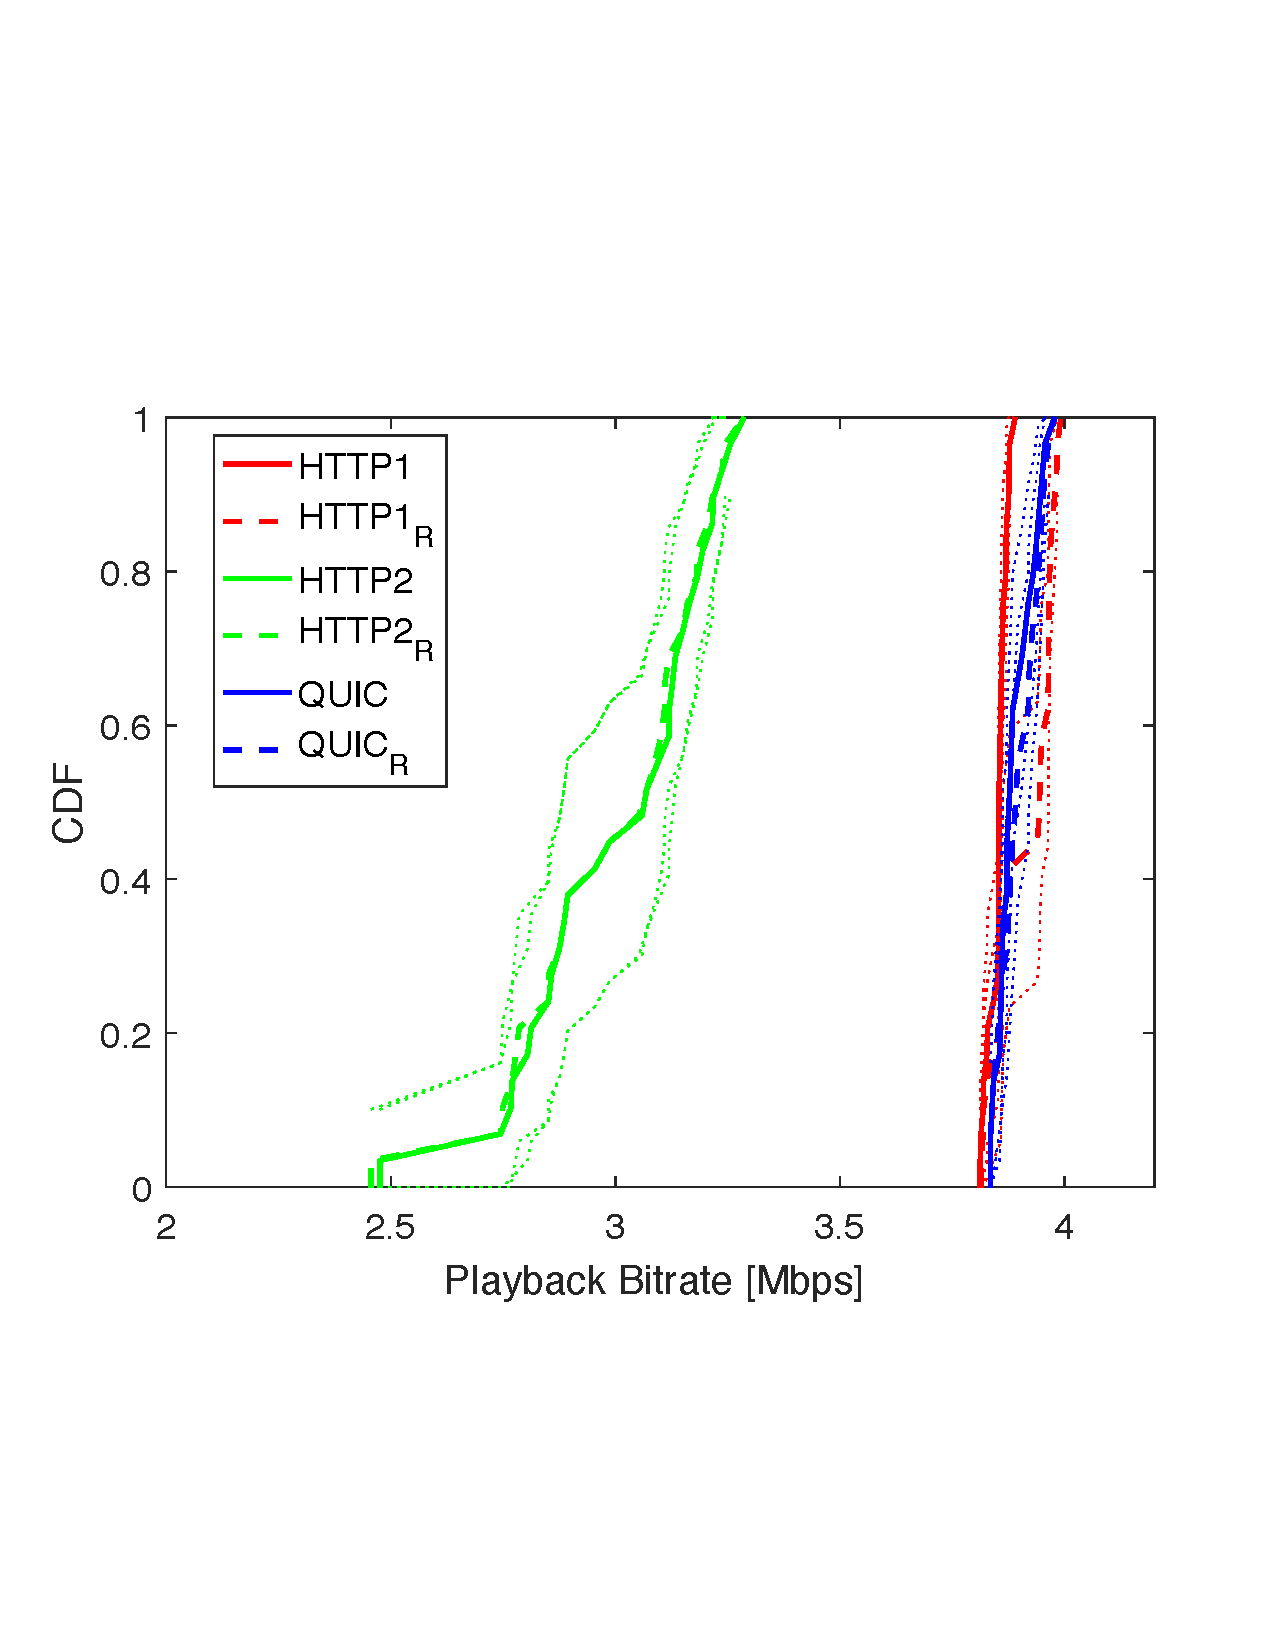
\includegraphics[trim={0 5cm 0 7cm}, scale=0.246]{figures/CDF_bitrat_squad_sdn_p1p2_nd18.pdf}
     \caption{}
    \label{fig:sdn_p1_p2bitrate}
  \end{subfigure}
  \begin{subfigure}[t]{0.33\textwidth}
  \captionsetup{justification=raggedright,singlelinecheck=false,margin=2.5cm}
    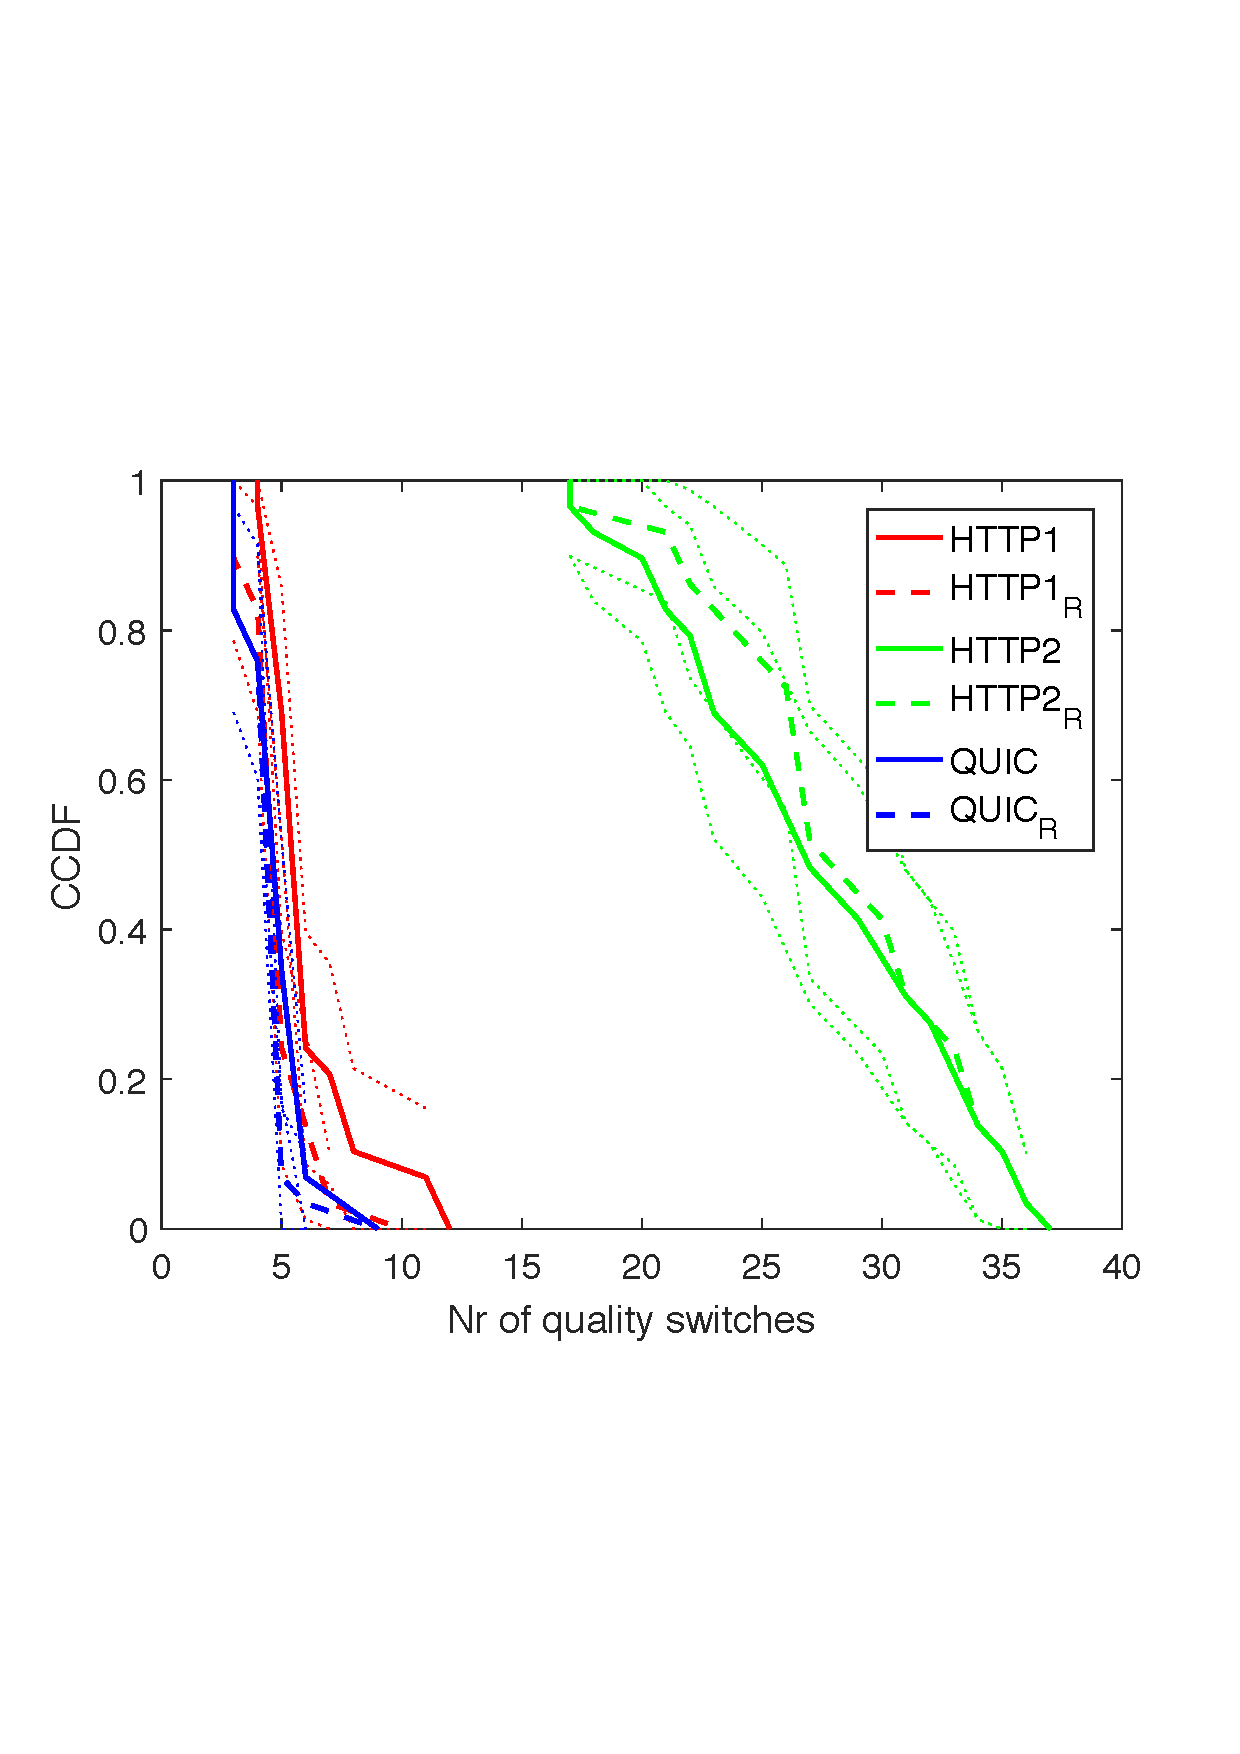
\includegraphics[trim={0 6cm 0 7cm}, scale=0.25]{figures/CDF_cntswitch_squad_sdn_p1p2_nd18.pdf}
    \caption{}
    \label{fig:sdn_p1_p2cntsw}
  \end{subfigure}
 % \begin{subfigure}[t]{0.4\textwidth}
  %\captionsetup{justification=centering,margin=0.5cm}
    %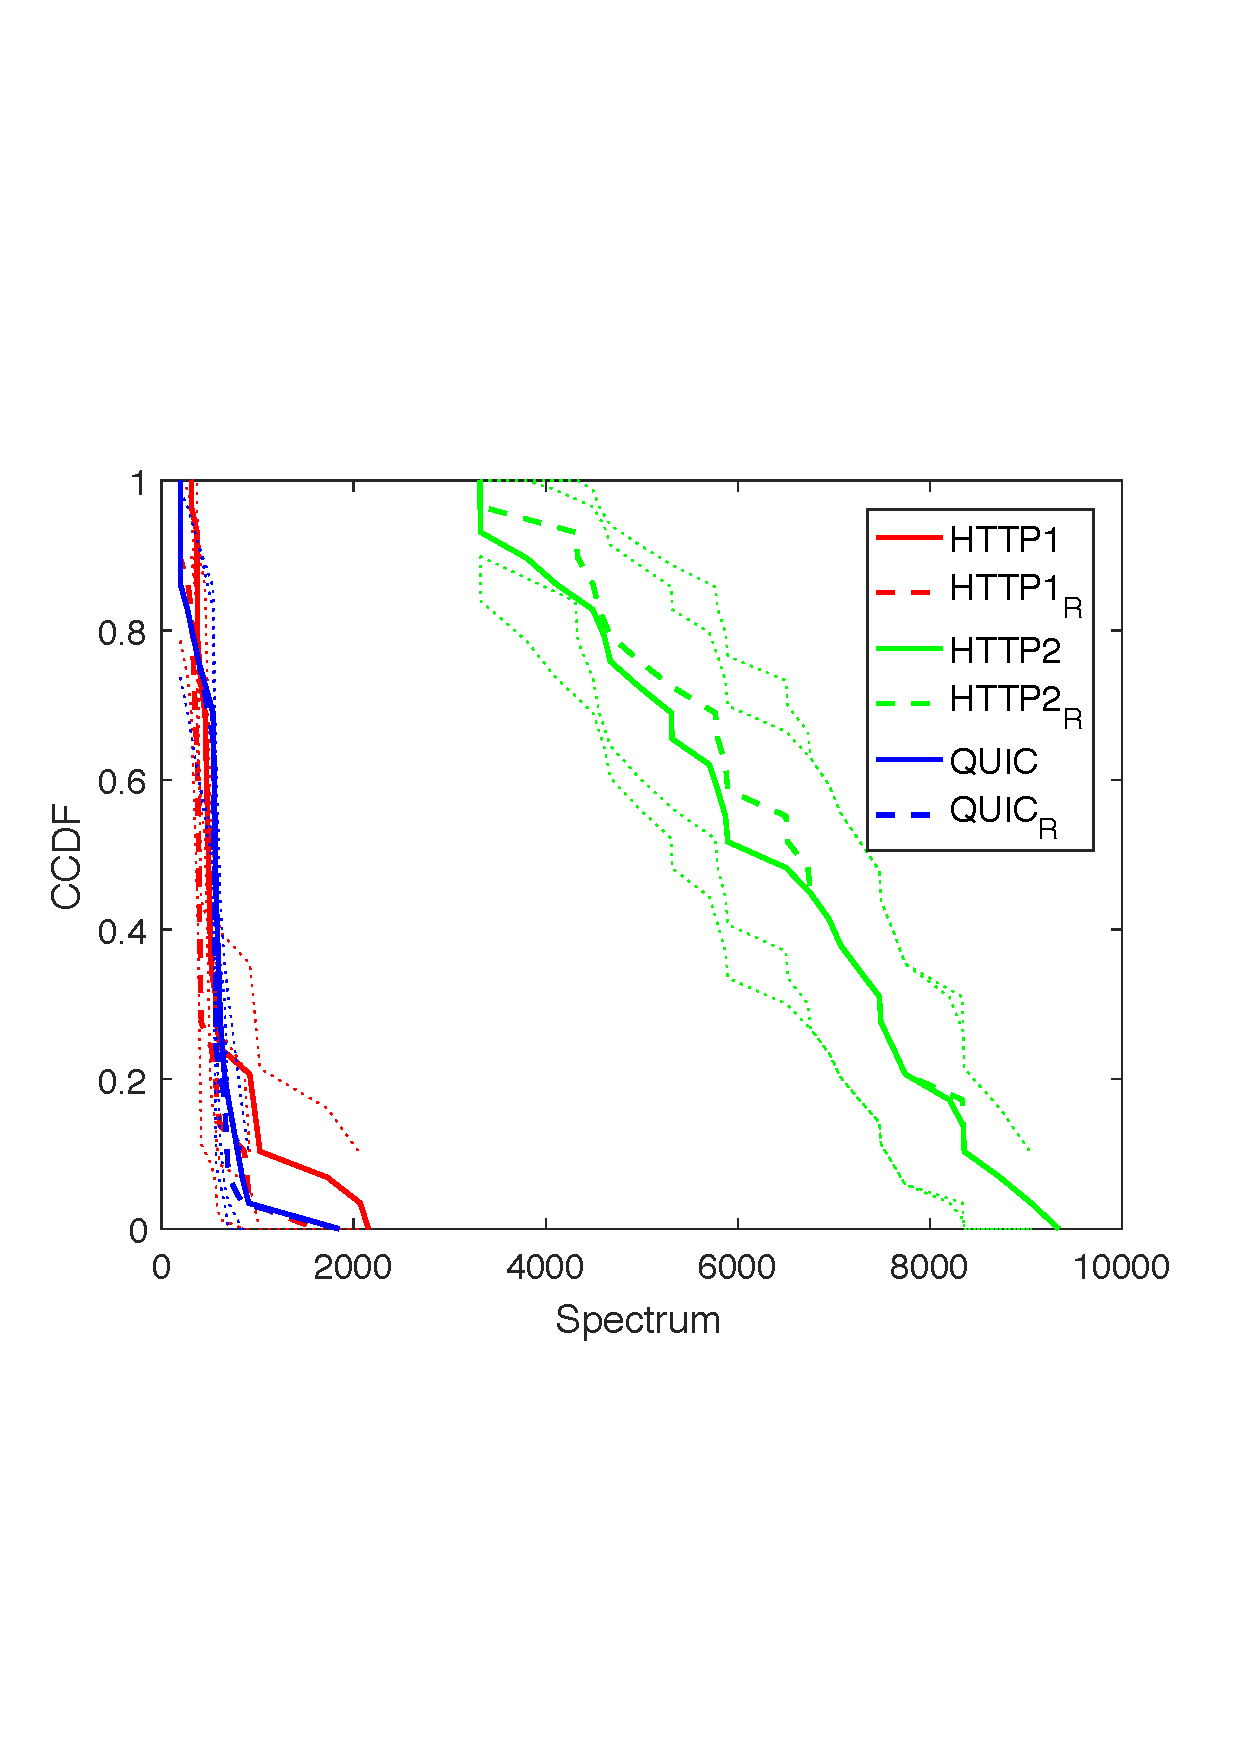
\includegraphics[trim={0 7cm 0 7cm}, scale=0.30]{figures/CDF_magswitch_squad_sdn_p1p2_nd18.pdf}
    %\caption{}
    %\label{fig:sdn_p1_p2magsw}
  %\end{subfigure}
    \begin{subfigure}[t]{0.33\textwidth}
  \captionsetup{justification=centering,margin=1.5cm}
    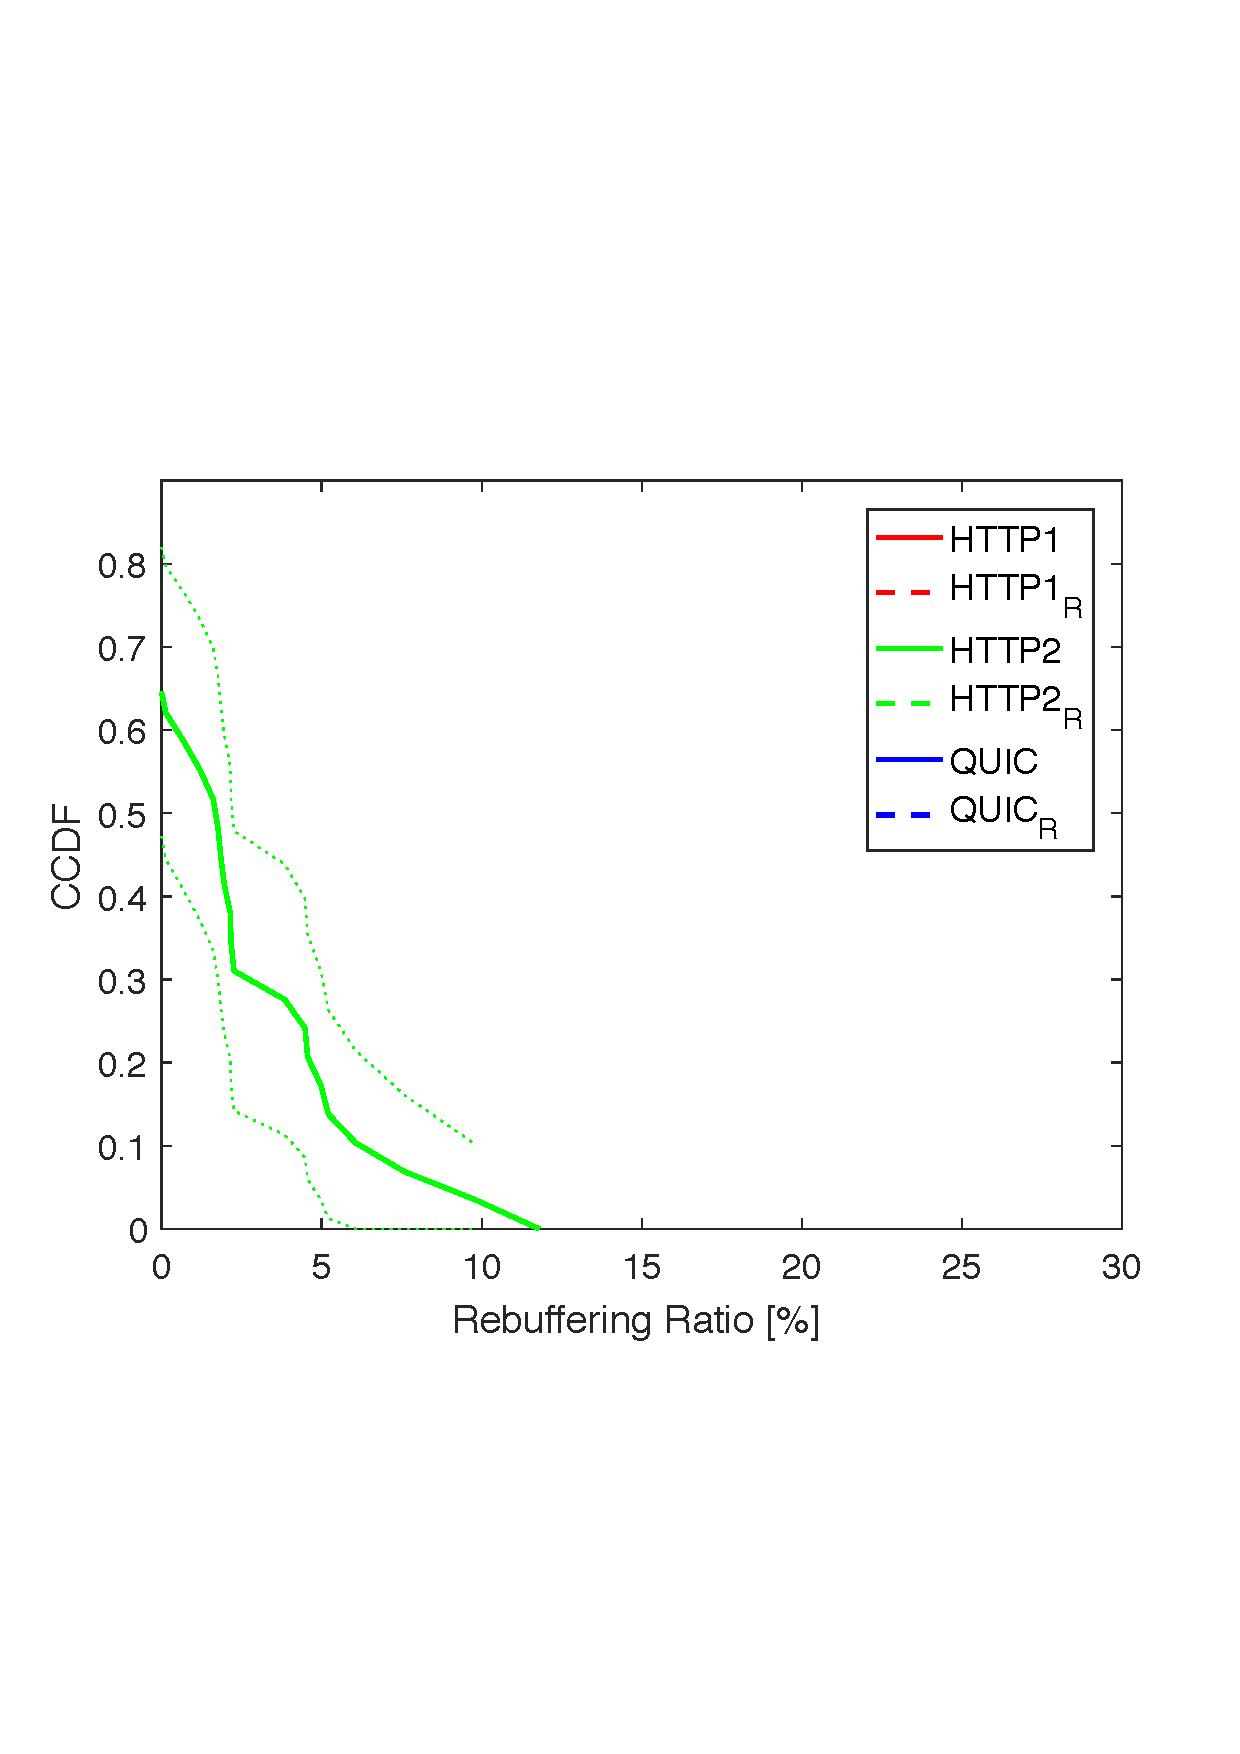
\includegraphics[trim={0 6cm 0 7cm}, scale=0.25]{figures/CDF_rebuffer_squad_sdn_p1p2_nd18.pdf}
    \caption{}
    \label{fig:sdn_p1_p2rebuf}
  \end{subfigure}
 \centering
  \vspace{-20pt}
  \caption{Single Client Measurements - Re-ordering and Head-of-Line Blocking. Re-ordering has an adverse effect on HTTP/2 causing significant degradation of QoE metrics, especially with respect to rebuffering which can be as high as 10\% in spite of selecting lower quality bitrates as seen from (a). Note, subscript ``R'' denotes ABR segment retransmissions.}
  \label{fig:sdn_p1_p2}
  \vspace{-10pt}
\end {figure*}
\ifdefined\flagTech
\begin{figure*}[htb!]
\centering
\begin{subfigure}[t]{0.35\textwidth}
   \captionsetup{justification=centering,margin=0cm}
     \hspace{-55pt}
    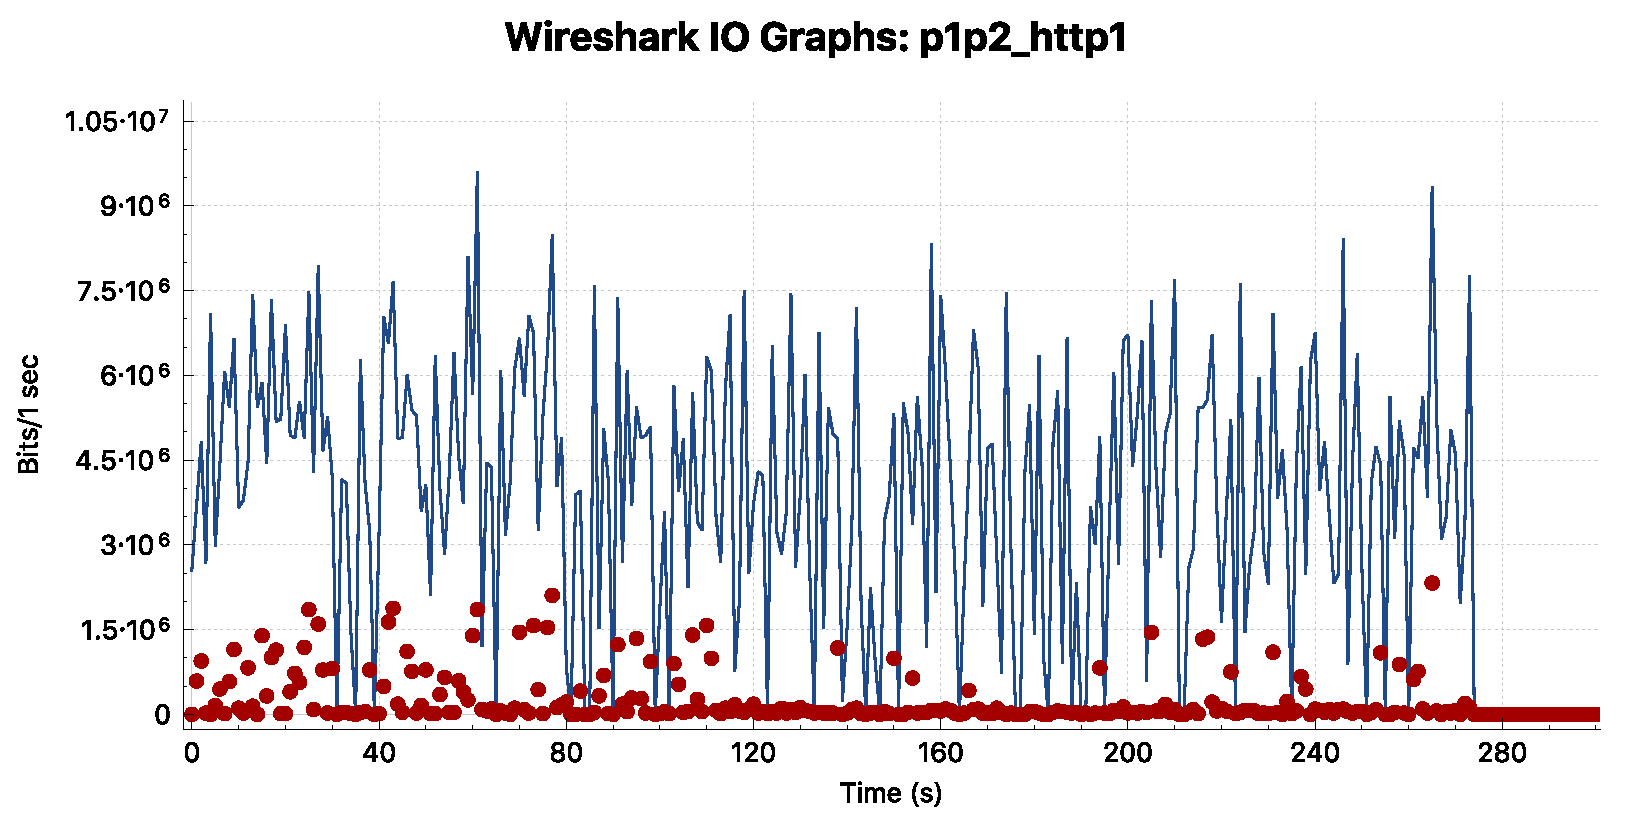
\includegraphics[scale=0.33, trim={100 0 0 0}]{figures/p1p2_http1.pdf}
     \caption{}
    \label{fig:sdn_p1_p2http1}
  \end{subfigure}
  \begin{subfigure}[t]{0.35\textwidth}
  \captionsetup{justification=raggedright,singlelinecheck=false,margin=2.5cm}
    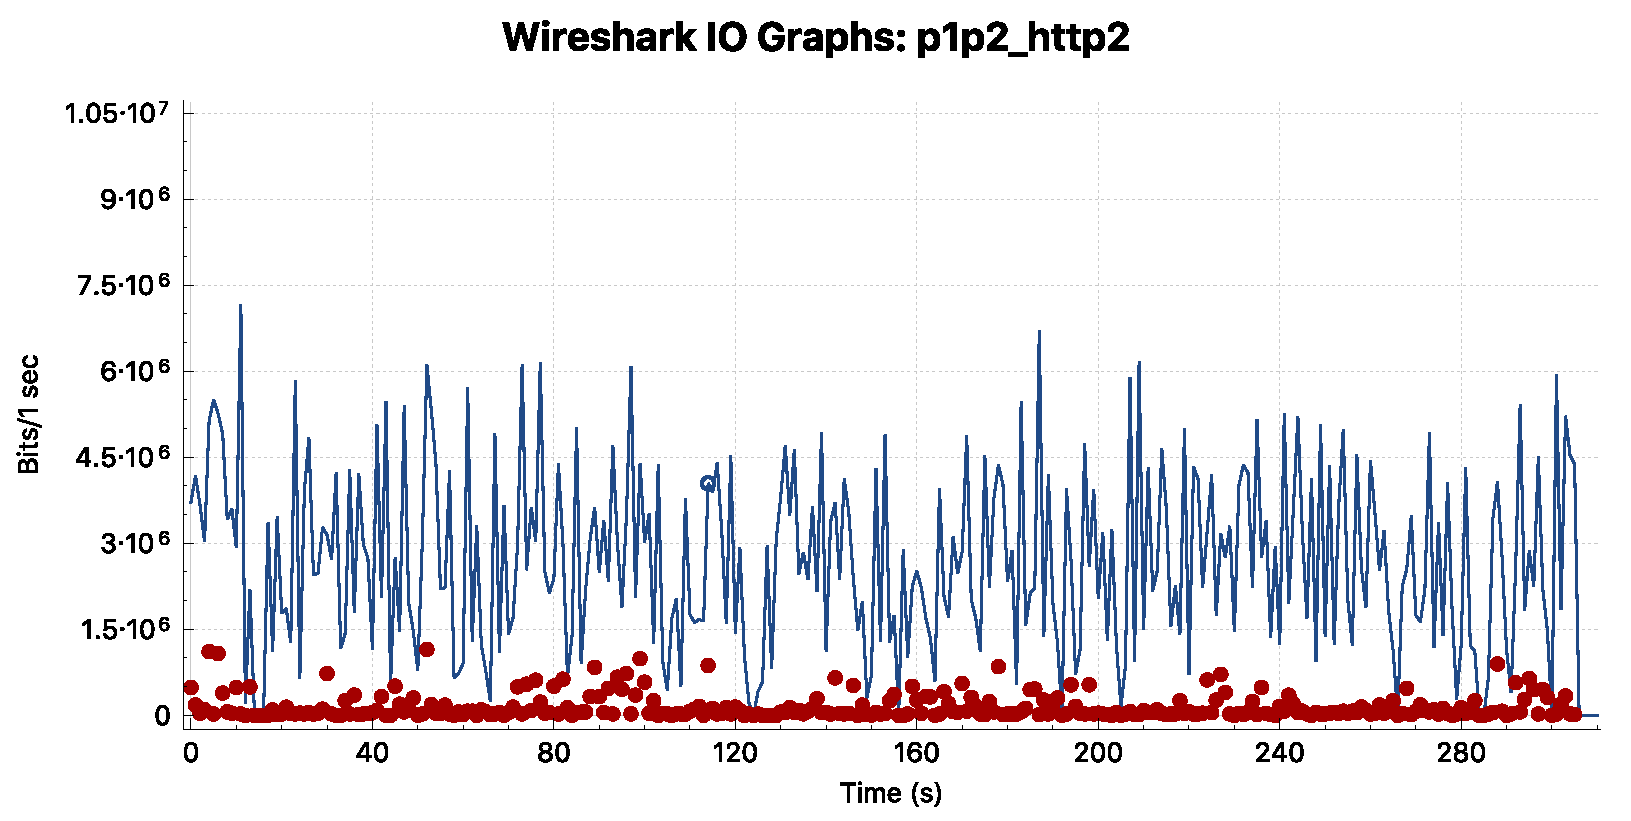
\includegraphics[scale=0.33, trim={25 0 0 0}]{figures/p1p2_http2.pdf}
    \caption{}
    \label{fig:sdn_p1_p2http2}
  \end{subfigure}
    \begin{subfigure}[t]{0.35\textwidth}
  \captionsetup{justification=centering,margin=1.5cm}
    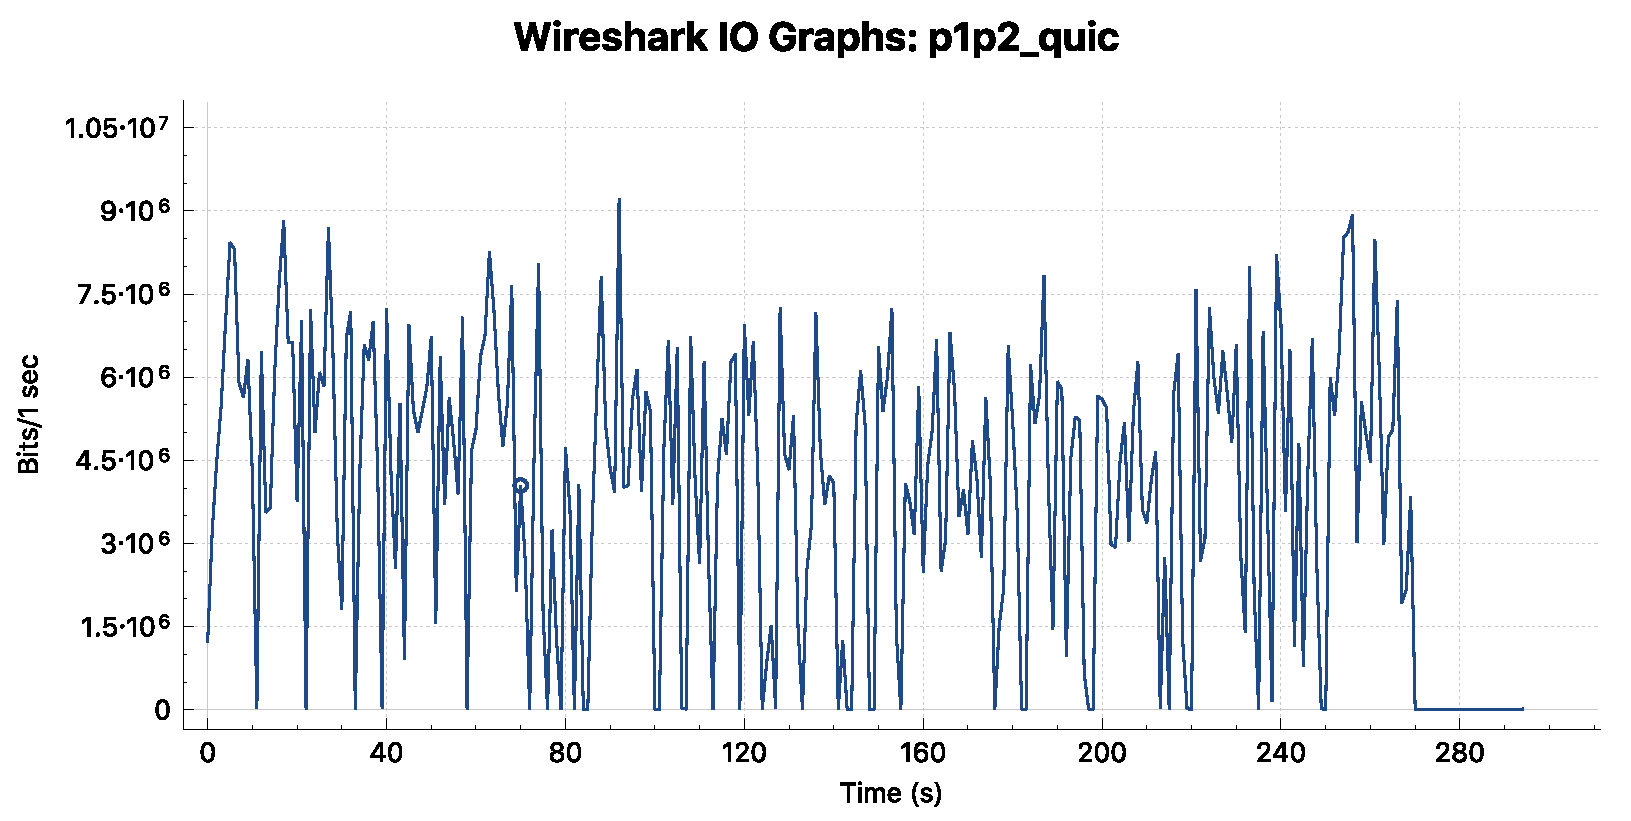
\includegraphics[scale=0.33,trim={150 0 0 0}]{figures/p1p2_quic.pdf}
    \caption{}
    \label{fig:sdn_p1_p2quic}
  \end{subfigure}
 \centering
  \caption{Single Client Measurements - Re-ordering and Head-of-Line Blocking. \texttt{Tshark} traces for one sample show that HTTP1.1 and HTTP2 experience significant TCP fast retransmits which cause QoE degradation when compared to QUIC.}
  \label{fig:sdn_p1_p2_wireshark}
 \vspace{-10pt}
\end {figure*}
\fi
Since packet reordering in the Internet is not uncommon~\cite{Jaiswal:TON:2007}, protocols for ABR streaming should be robust in the face of such reordering. Here, we study the ability of HTTP1.1, HTTP/2, and QUIC to recover from re-ordering of packets. This is the only experiment where we use the second path (denoted \textbf{P2} in Fig. \ref{fig:clab_topo}) to carry video streams. In order to induce re-ordering of packets, we switch between a low latency, low loss path, \textbf{P1}, and a high latency, high loss path, \textbf{P2}, every second using SDN, namely the OpenFlow \cite{mckeown2008openflow} implementation, which provides fine-grained, dynamic traffic engineering for application packets. As shown in Fig. \ref{fig:clab_topo}, \textbf{P2} is characterized by 1\% loss and 10ms delay implemented using \texttt{tc}\footnote{\url{http://lartc.org/manpages/tc.txt}} and \texttt{netem}\footnote{\url{http://man7.org/linux/man-pages/man8/tc-netem.8.html}} utilities. For the experiments presented in Sect.~\ref{subsubsec:single_udp}, we find that HTTP/2 is either comparable or marginally worse than HTTP/1.1 and QUIC. In the case of packet reordering (shown in Figure \ref{fig:sdn_p1_p2}), we see that HTTP/2 performs significantly worse than QUIC and HTTP/1.1 . Not only is the $AQB$ significantly lower with a high variation between runs, but also the rebuffering is as high as 10\% where over 60\% of clients experience an $RB$ of ~2.5\%. Further analysis using the \texttt{tshark}\footnote{\url{https://www.wireshark.org/docs/man-pages/tshark.html}} utility reveals that a HTTP/2 session experiences 9.5\% fast TCP retransmits. In comparison, HTTP/1.1 experiences 7.1\%, and QUIC sessions experience no UDP retransmissions since they use NACKs (c.f. Sect. \ref{subsubsec:quicvstcp}). More details on the \texttt{tshark} data can be found in~\cite{QUIC_TR:2018}
\ifdefined\flagTech \DB{Fig. \ref{fig:sdn_p1_p2_wireshark}. Here, we take the example of one run to show that HTTP1.1 and HTTP/2 experience several fast retransmits as compared to QUIC.} \fi Additionally, QUIC uses a higher initial congestion window size=32 (the Linux default for TCP is 10) and also grows the window more aggressively, thus, allowing more unacknowledged bytes in flight. This results in a more reliable download rate measurement and a stable buffer level for the ABR client and consequently, a reduction in the quality variations $\#QS$ as observed in Fig. \ref{fig:sdn_p1_p2cntsw}. 

\subsubsection{Parallel Clients: Competing Traffic}
For this experiment we use the additional client and server pairs (denoted as \textit{Client2}/\textit{Server2} and \textit{Client3}/\textit{Server3} in Figure \ref{fig:clab_topo}) to initiate three simultaneous sessions of QUIC-based SQUAD clients. Although all three clients enjoy a smooth playback experience without rebuffering as shown in Figure \ref{fig:pquic}, we note that the bandwidth sharing can result in unfair behavior in the case of ABR streaming sessions. This is contrary to the analysis presented by the authors of \cite{Kakhki:IMC:2017} where they observe that QUIC flows are fair to each other but only unfair to TCP flows when downloading a file. While we similarly observe that QUIC does tend to "starve out" TCP flows, we note that ABR streaming over QUIC with the use of retransmissions can result in unfair behavior for competing ABR streams since multiplexing due to retransmissions can occur at different points throughout the streaming session. In order to corroborate this analysis, we present the percentage of retransmissions in Table \ref{tab:retx_parallel_quic}, which shows that the three clients experience varying number of ABR segment retransmissions per run. Since these retransmissions occur asynchronously, the clients observe different buffer levels and rate measurements throughout a streaming session. We also perform similar experiments with three HTTP/2 clients and observe that HTTP/2 shows a nearly equal distribution of $AQB$ and closer inspection reveals that the $AQB$ of \textit{Client1} is 0.5Mbps higher on average as compared to the other two clients. Since TCP is more conservative about setting the initial congestion window size and has a less aggressive window growth it enables all three clients to have a "fair" share of the bottleneck bandwidth. Further details on the TCP-based experiments can be found in~\cite{QUIC_TR:2018}.
\ifdefined\flagTech \DB{Figure \ref{fig:phttp1} shows the QoE metrics for a case with three concurrent ABR clients and Figure \ref{fig:phttp2} shows similar results for three parallel HTTP/2 clients. Although none of the clients experience rebuffering in both cases, for HTTP1.1 clients, we see that one client obtains a very high bitrate compared to the others. Since the retransmissions do not occur simultaneously with original segment downloads in the HTTP1.1 case, we note that this creates significant heterogeneity in the bitrate of sequential requests made by various clients. We do not observe such an affect in the case of HTTP/2 since the retransmissions are multiplexed with original segments and TCP naturally ensures fairness. After understanding the concurrent behavior of HTTP1.1, HTTP2 and QUIC individually, we present one case where each of these three protocols compete with each other in Fig. \ref{fig:pmixed} which reveals that  HTTP1.1 and QUIC sessions have a relatively high QoE when compared to HTTP/2 sessions, which experience rebuffering as high as 23\% in addition to low quality bitrates, which leads us to conclude that the multiplexing feature of HTTP/2 is severely limited by underlying TCP parameters that need to be better tuned to support such a feature in order to obtain a better QoE performance.}\fi
\label{subsubsec:parallel}
\begin{figure*}[t!]
\centering
\begin{subfigure}[t]{0.33\textwidth}
   \captionsetup{justification=centering,margin=4.5cm}
    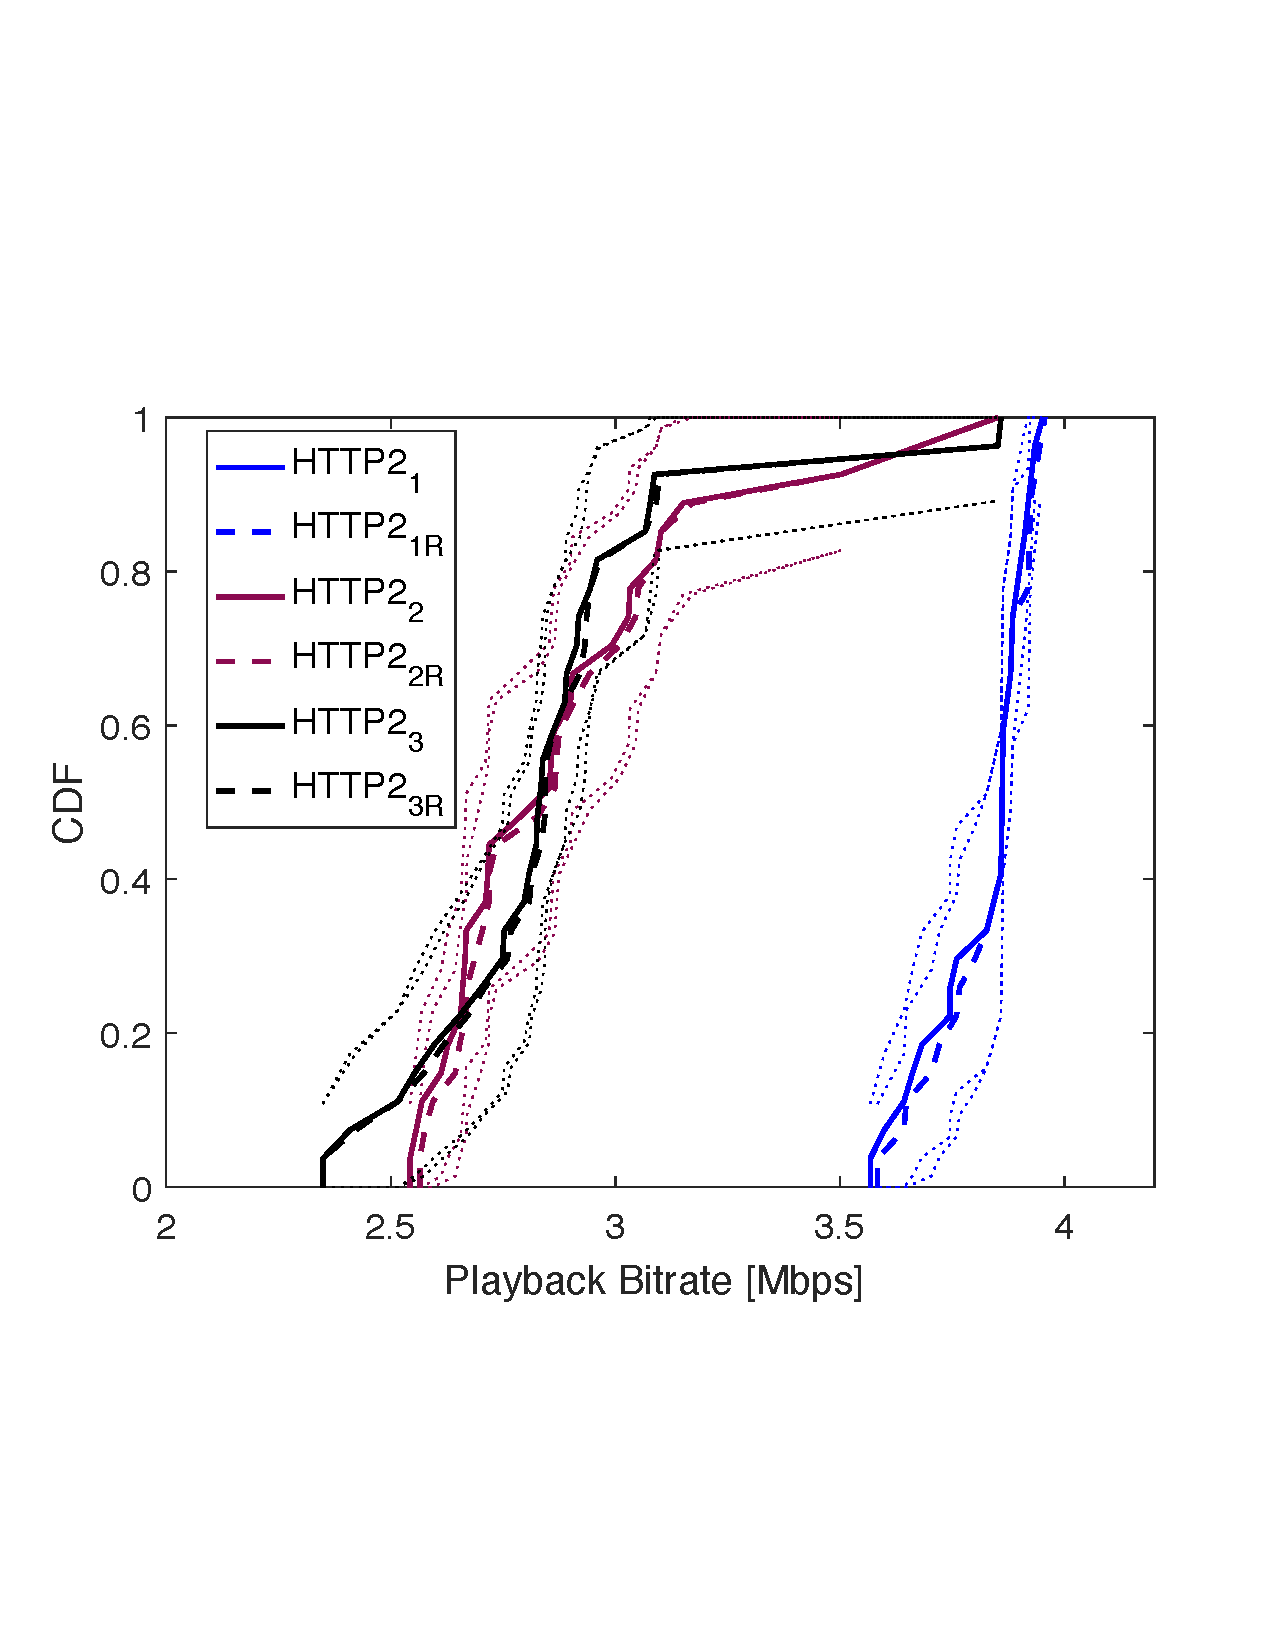
\includegraphics[trim={0 6cm 0 7cm}, scale=0.246]{figures/CDF_bitrat_squad_parallel_quic_nd18.pdf}
     \caption{}
    \label{fig:pquicbitrate}
  \end{subfigure}
  \begin{subfigure}[t]{0.33\textwidth}
  \captionsetup{justification=raggedright,singlelinecheck=false,margin=2.5cm}
    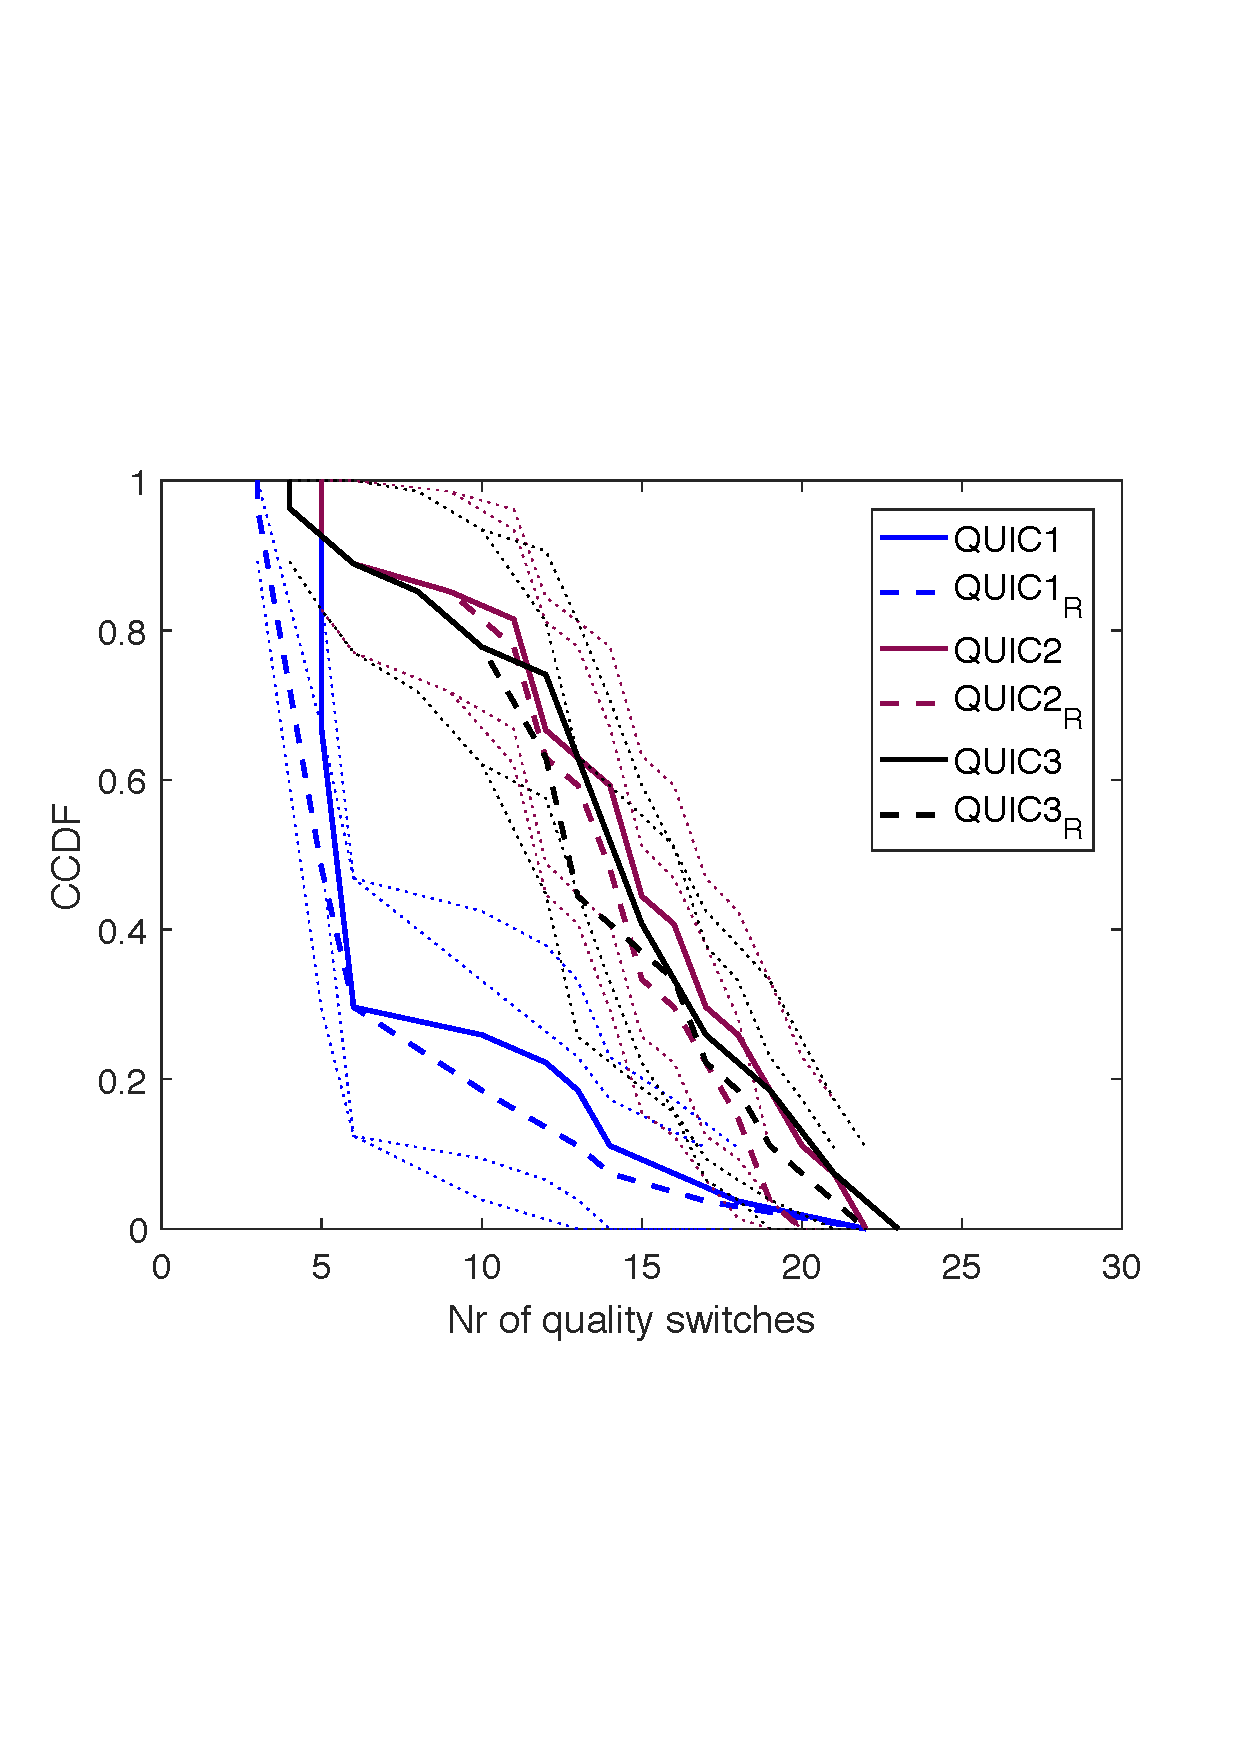
\includegraphics[trim={0 7cm 0 7cm}, scale=0.25]{figures/CDF_cntswitch_squad_parallel_quic_nd18.pdf}
    \caption{}
    \label{fig:pquiccntsw}
  \end{subfigure}
  \begin{subfigure}[t]{0.33\textwidth}
  \captionsetup{justification=centering,margin=1.5cm}
    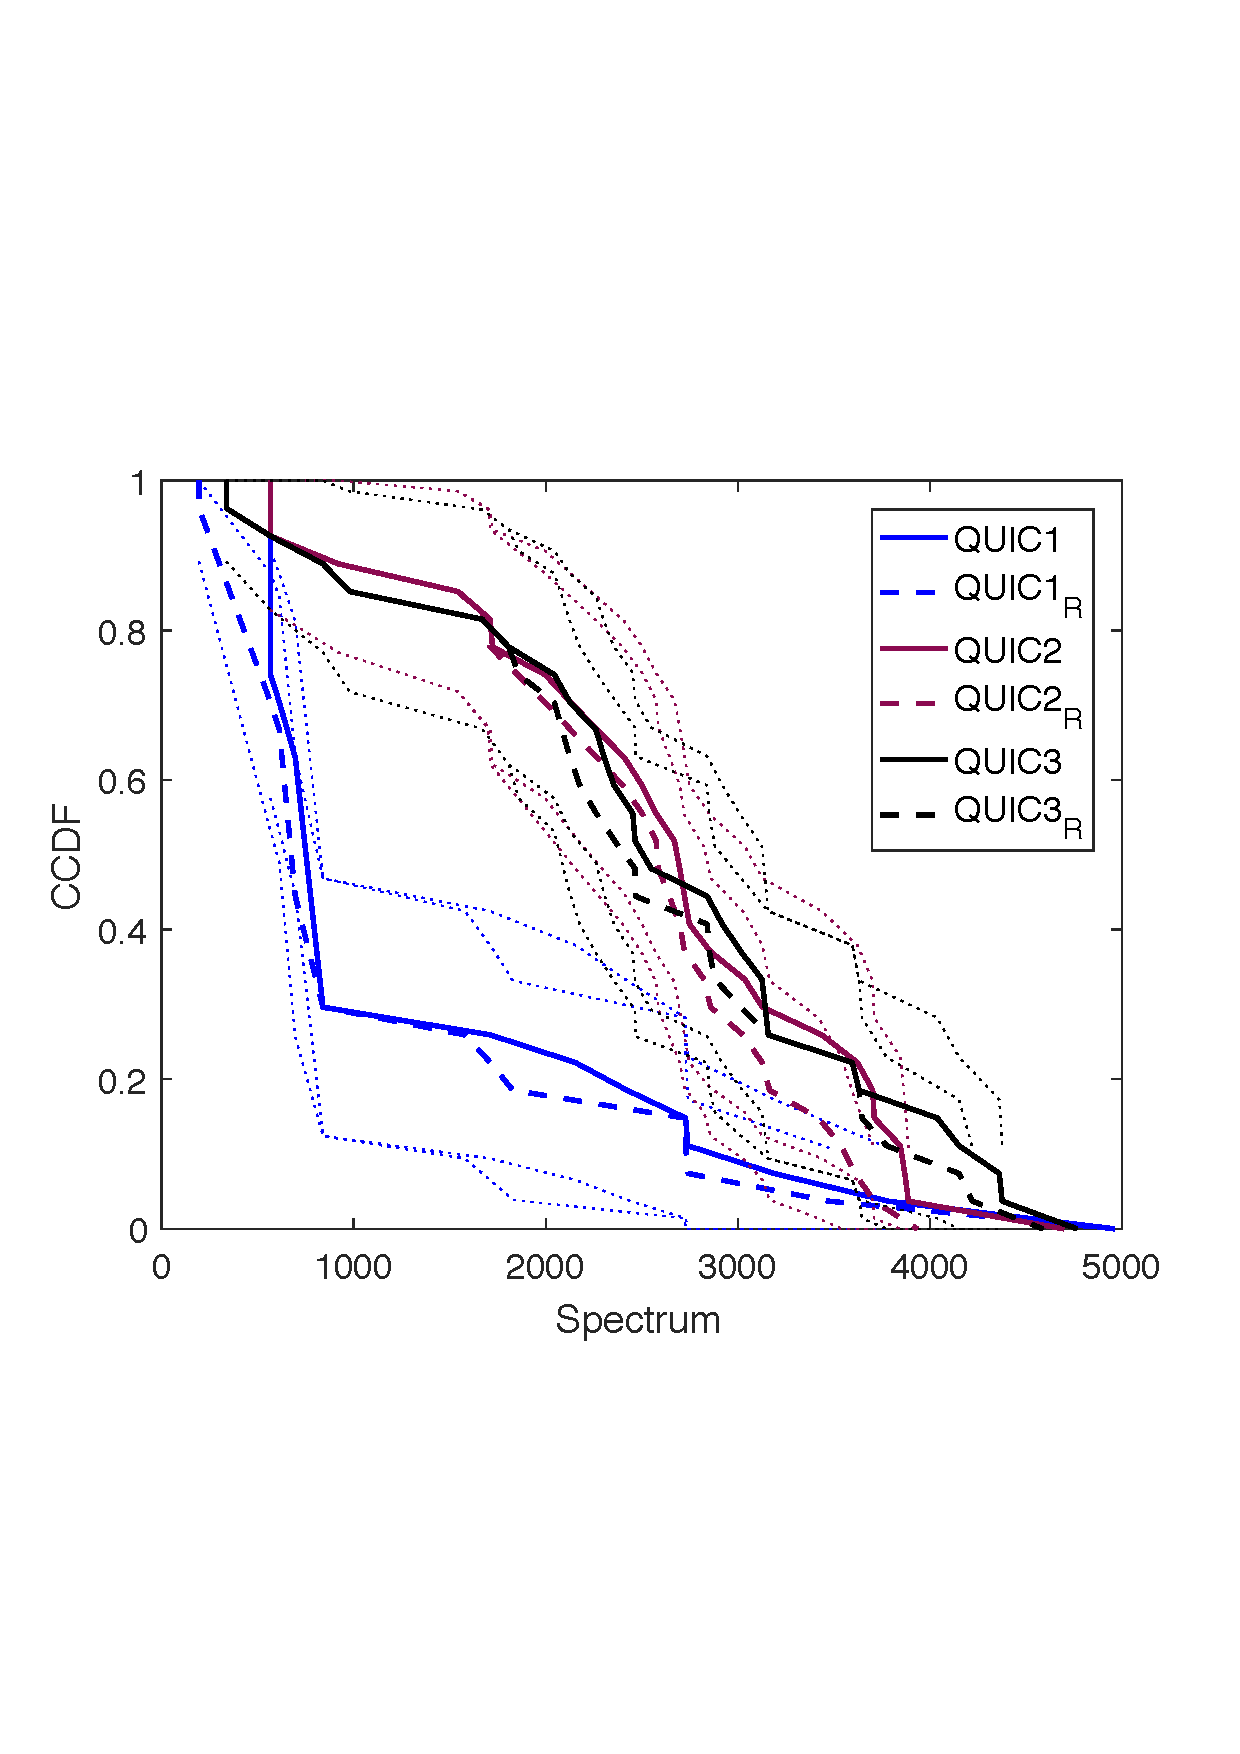
\includegraphics[trim={0 7cm 0 7cm}, scale=0.25]{figures/CDF_magswitch_squad_parallel_quic_nd18.pdf}
    \caption{}
    \label{fig:pquicmagsw}
  \end{subfigure}
 \centering
    \vspace{-15pt}
  \caption{Parallel Client Measurements - Three QUIC Clients. Competing QUIC clients show an unfair behavior where two clients experience relatively similar QoE but one client has a significantly better QoE than others.}
  \label{fig:pquic}
  \vspace{-10pt}
\end {figure*}
\ifdefined\flagTech
\begin{figure*}[t!]
\centering
\begin{subfigure}[t]{0.33\textwidth}
   \captionsetup{justification=centering,margin=4.5cm}
    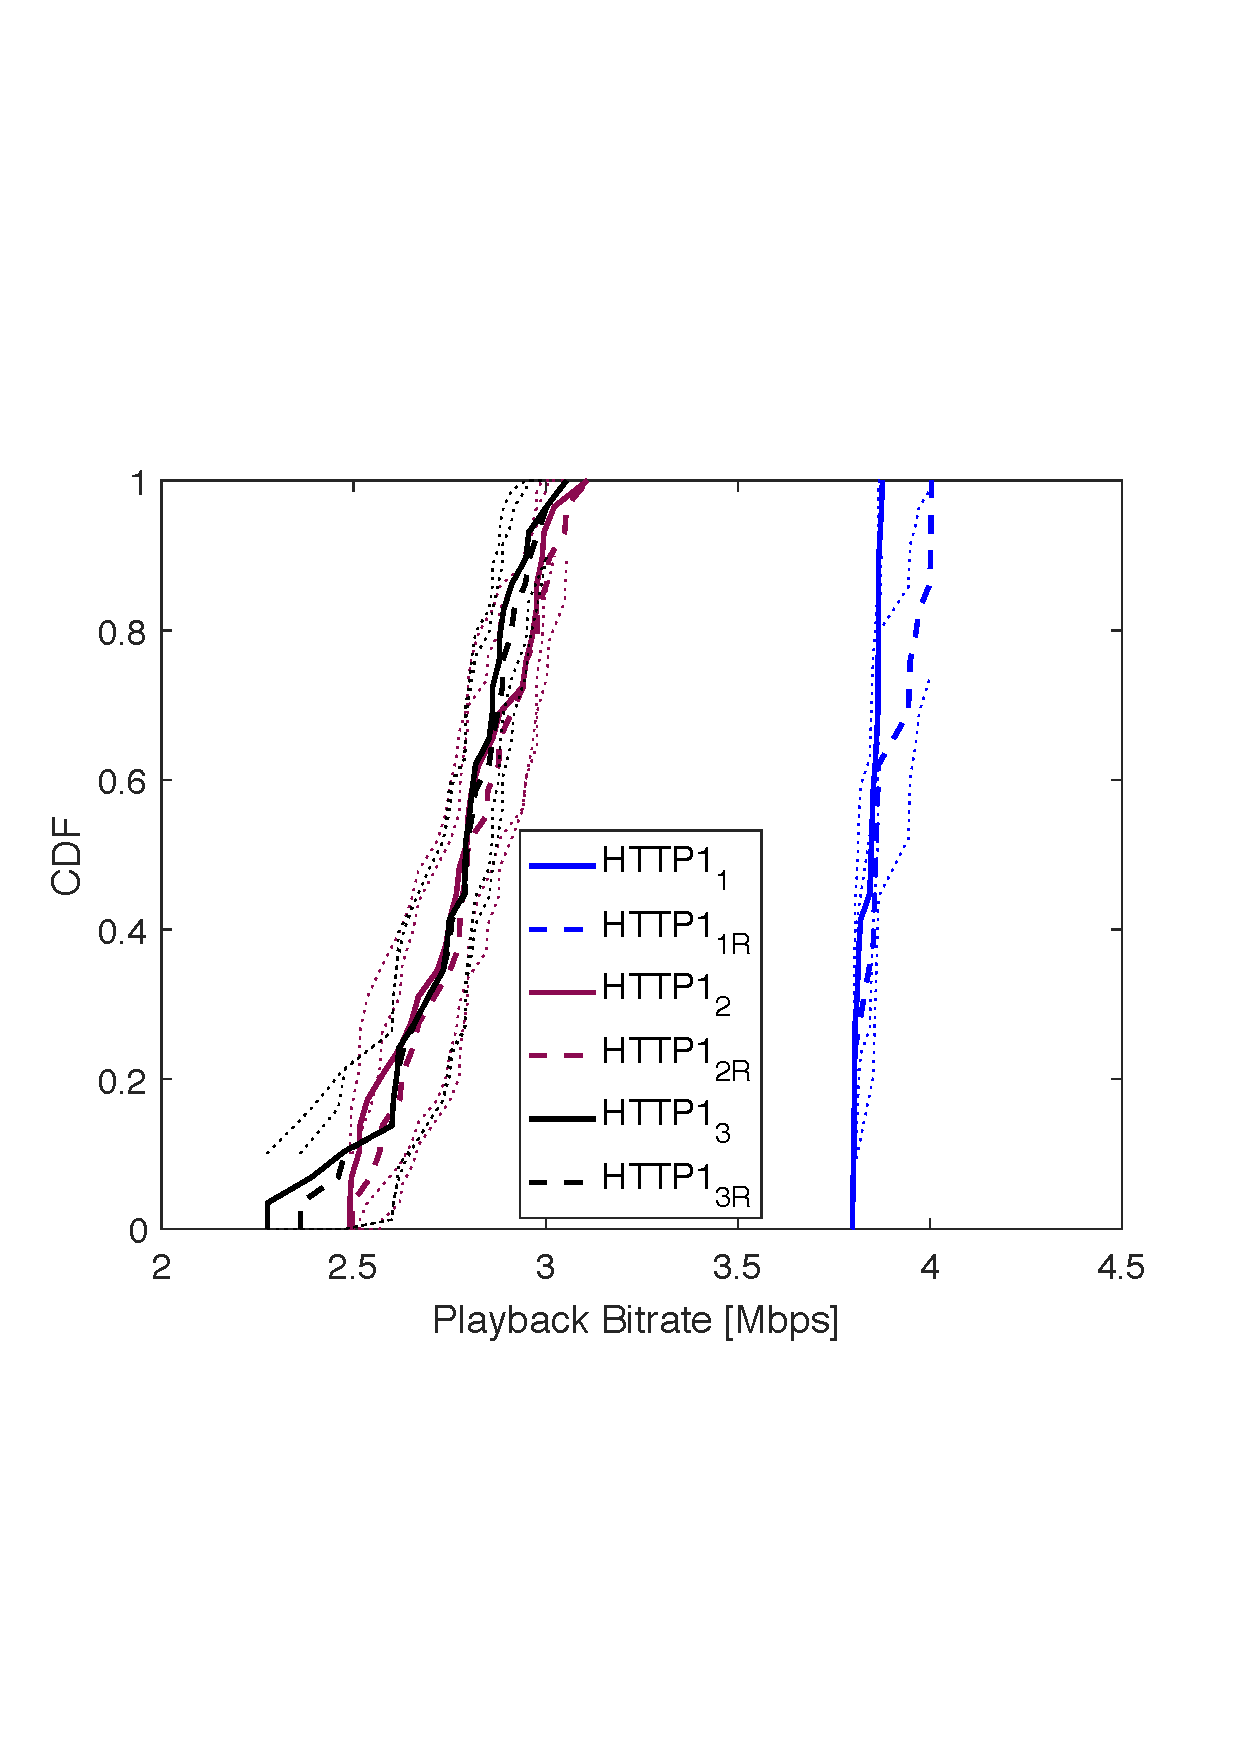
\includegraphics[trim={0 7cm 0 7cm}, scale=0.25]{figures/CDF_bitrat_squad_parallel_http1_nd18.pdf}
     \caption{}
    \label{fig:phttp1bitrate}
  \end{subfigure}
  \begin{subfigure}[t]{0.33\textwidth}
  \captionsetup{justification=raggedright,singlelinecheck=false,margin=2.5cm}
    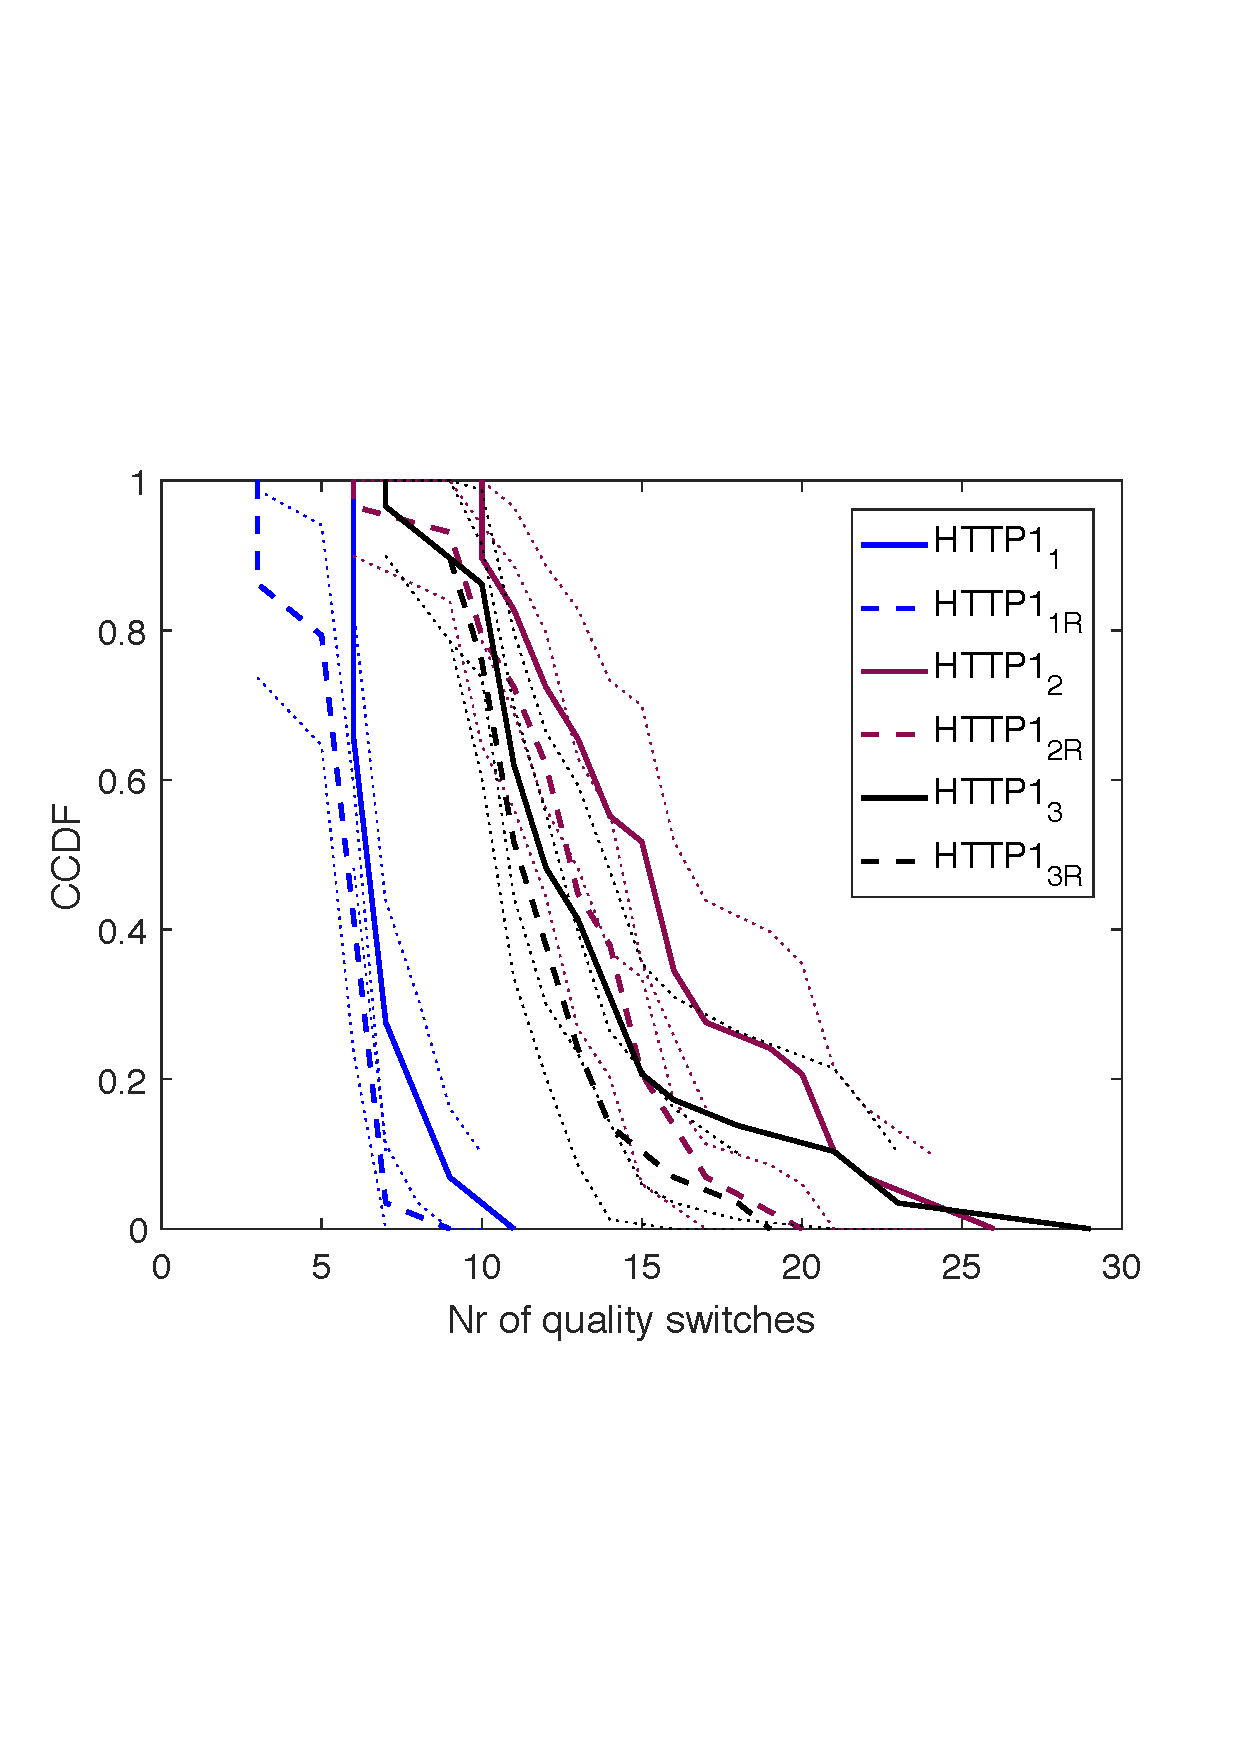
\includegraphics[trim={0 7cm 0 7cm}, scale=0.25]{figures/CDF_cntswitch_squad_parallel_http1_nd18.pdf}
    \caption{}
    \label{fig:phttp1cntsw}
  \end{subfigure}
  \begin{subfigure}[t]{0.33\textwidth}
  \captionsetup{justification=centering,margin=1.5cm}
    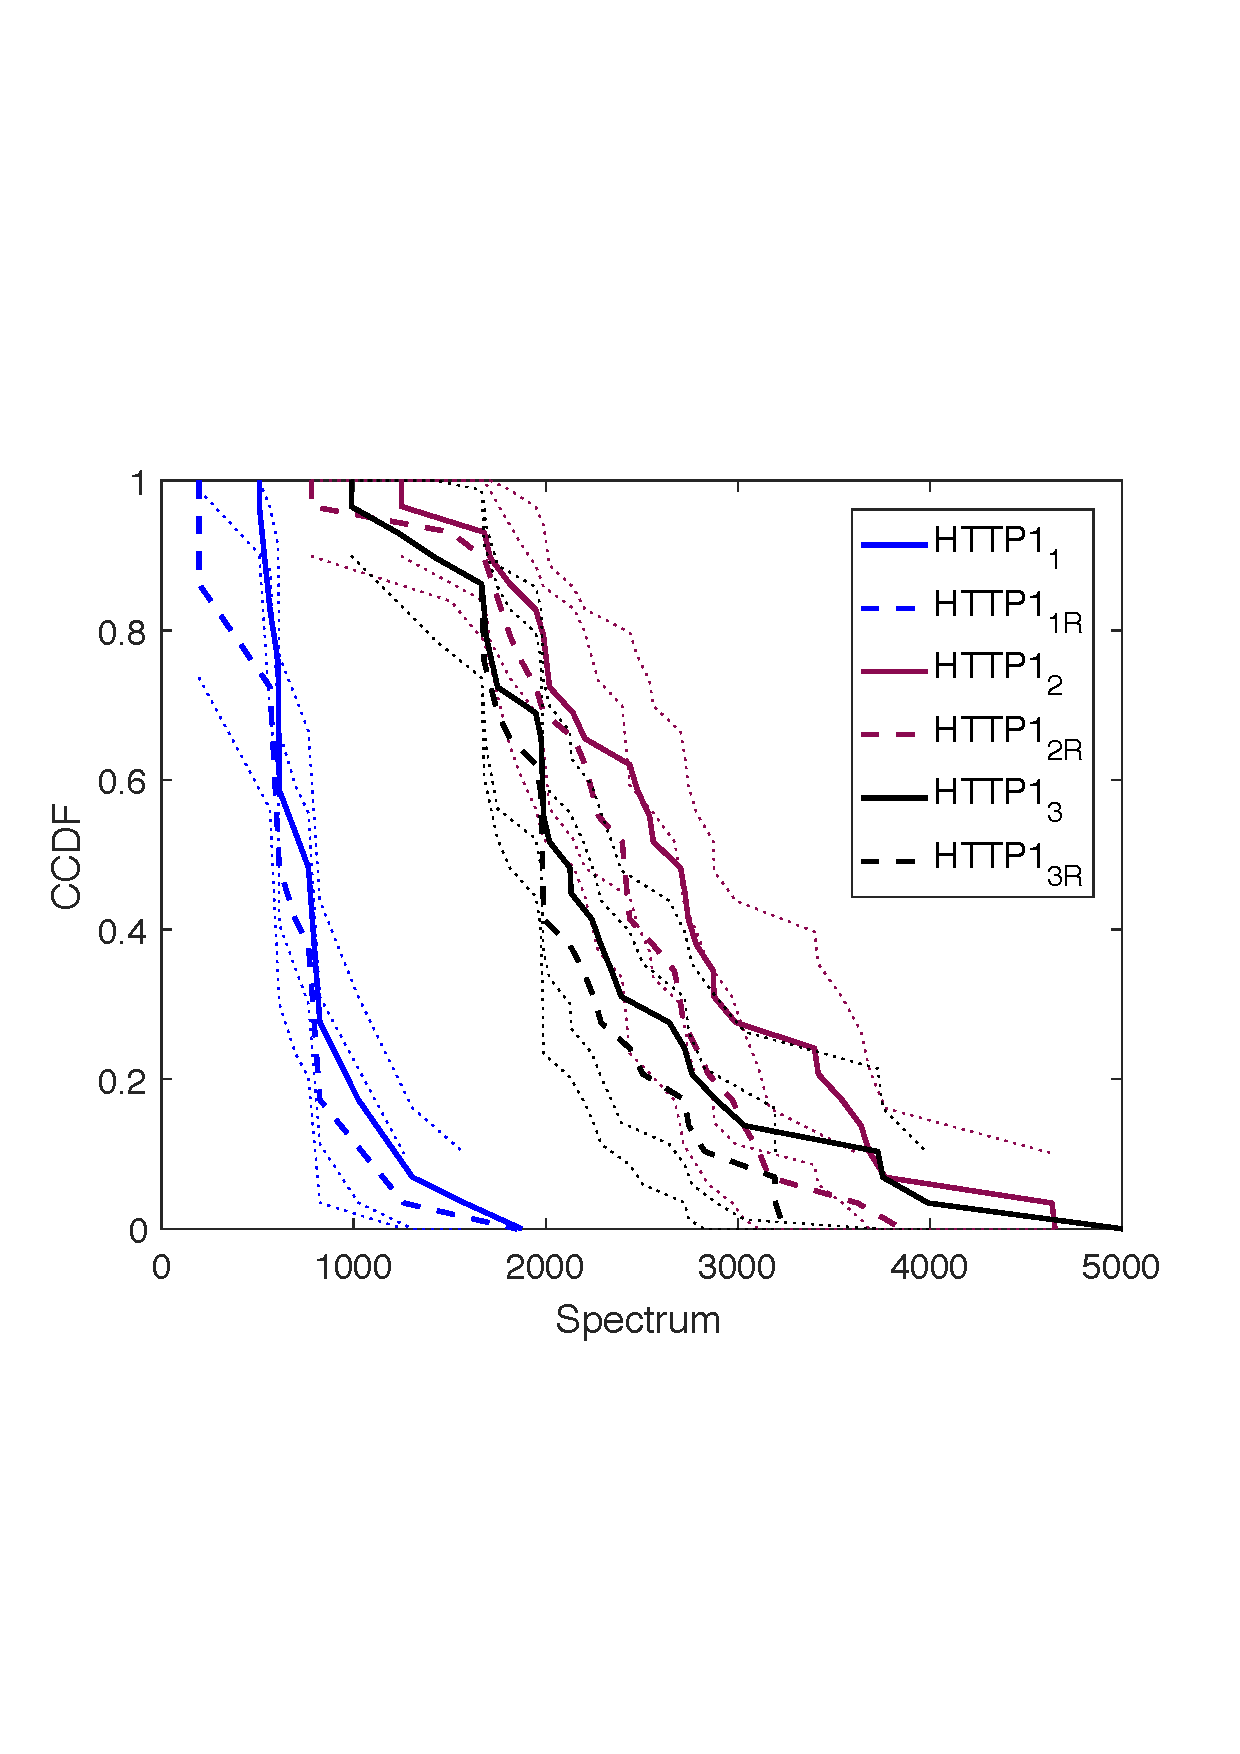
\includegraphics[trim={0 7cm 0 7cm}, scale=0.25]{figures/CDF_magswitch_squad_parallel_http1_nd18.pdf}
    \caption{}
    \label{fig:phttp1magsw}
  \end{subfigure}
 \centering
  \caption{Parallel Client Measurements - Three HTTP1.1 Clients. Client 1 experiences a significantly higher QoE. Since HTTP1.1 does not support multiplexing, the clients request segments of heterogenous quality bitrates sequentially causing the QoE performance to be significantly different.}
  \label{fig:phttp1}
\end {figure*}
\begin{figure*}[t!]
\centering
\begin{subfigure}[t]{0.33\textwidth}
   \captionsetup{justification=centering,margin=4.5cm}
    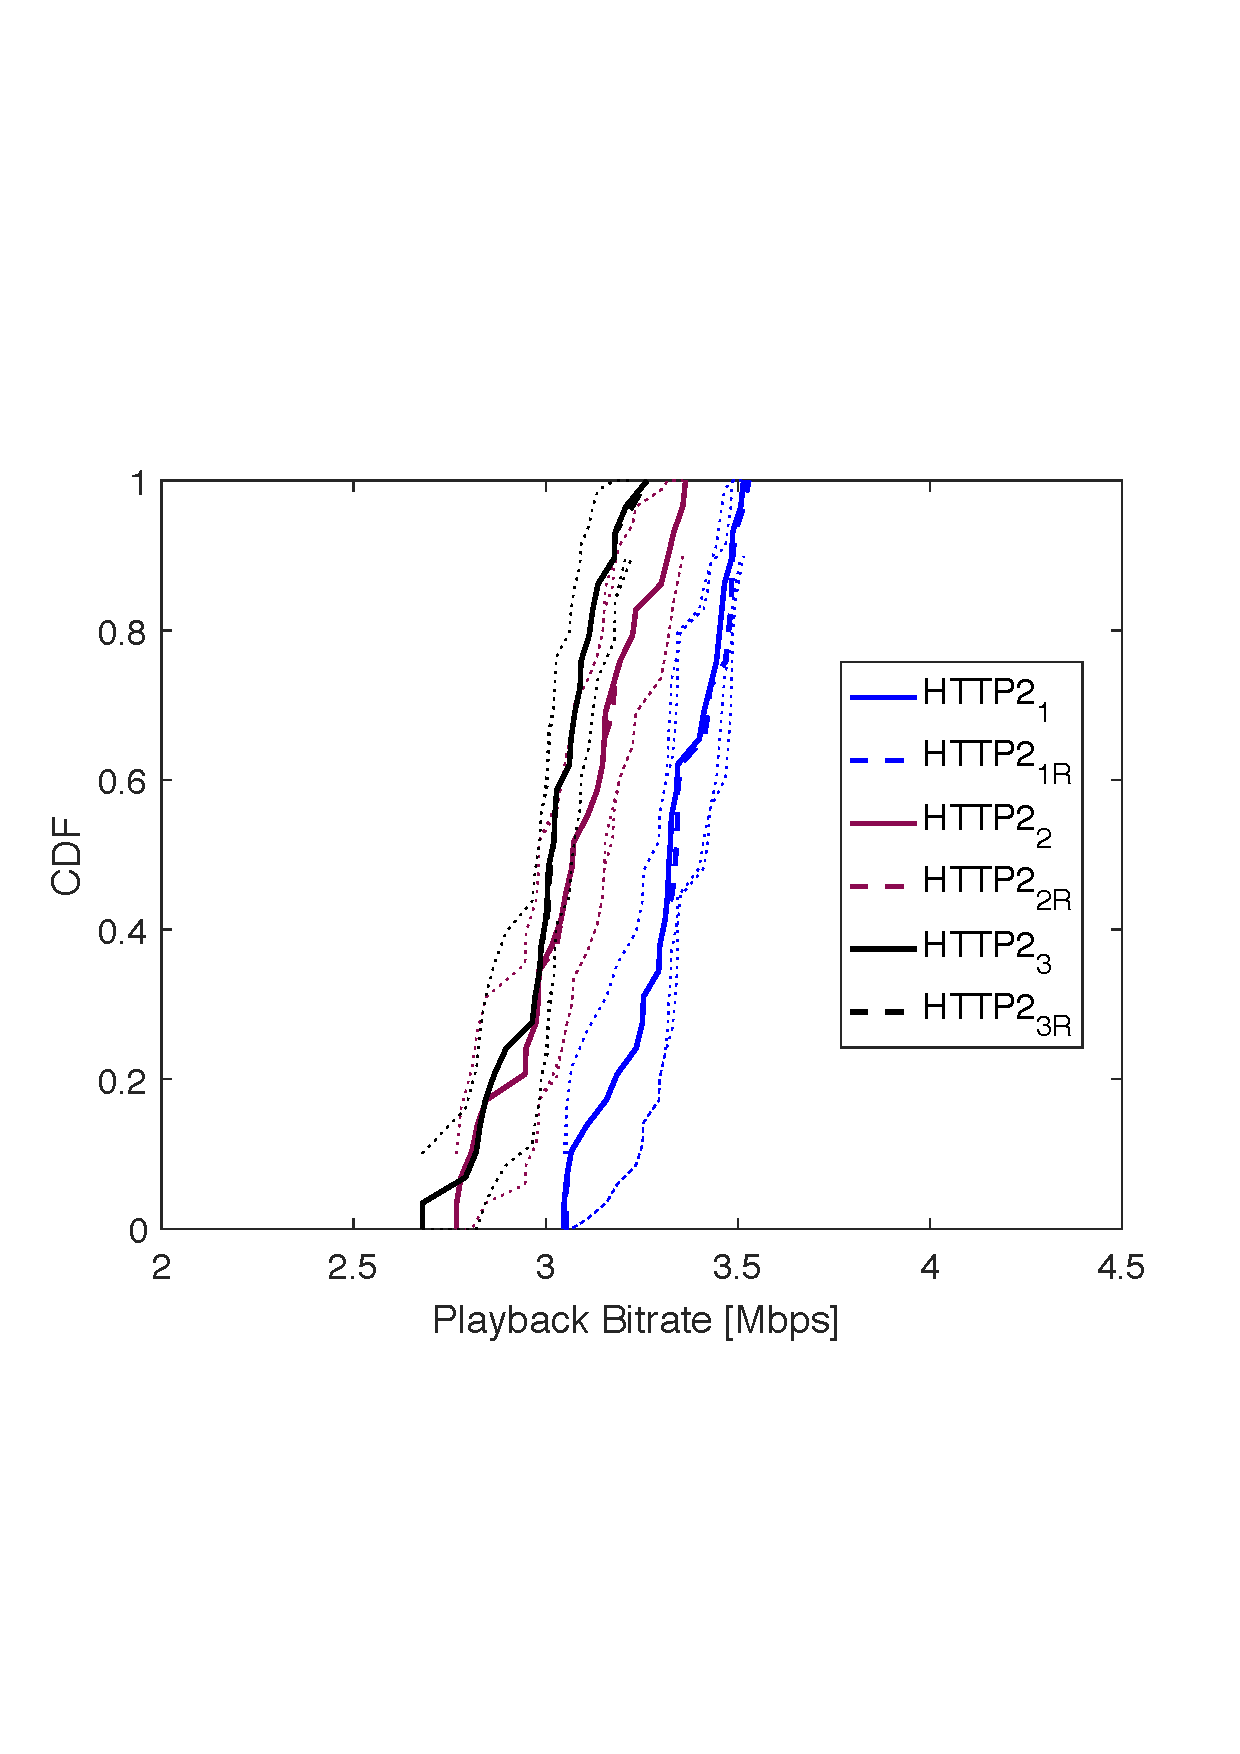
\includegraphics[trim={0 7cm 0 7cm}, scale=0.25]{figures/CDF_bitrat_squad_parallel_http2_nd18.pdf}
     \caption{}
    \label{fig:phttp2bitrate}
  \end{subfigure}
  \begin{subfigure}[t]{0.33\textwidth}
  \captionsetup{justification=raggedright,singlelinecheck=false,margin=2.5cm}
    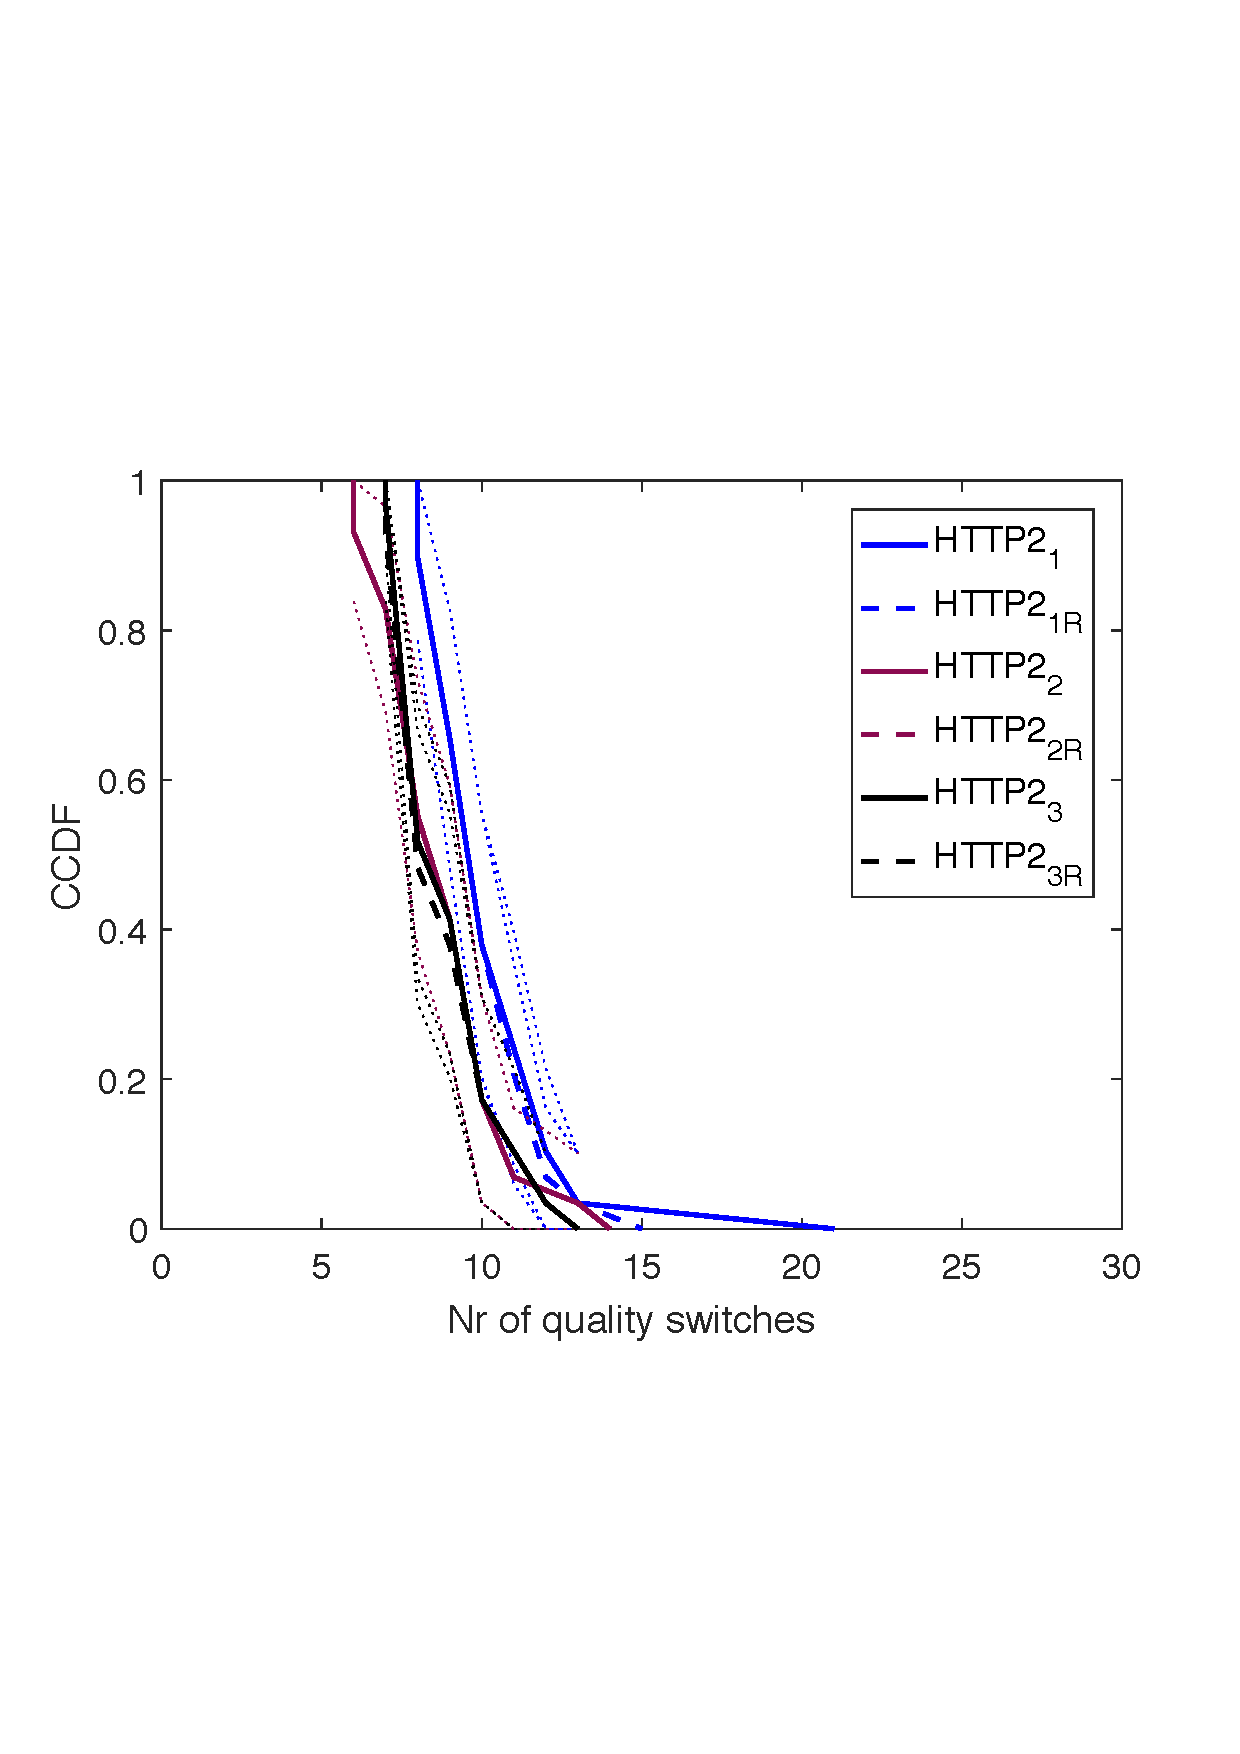
\includegraphics[trim={0 7cm 0 7cm}, scale=0.25]{figures/CDF_cntswitch_squad_parallel_http2_nd18.pdf}
    \caption{}
    \label{fig:phttp2cntsw}
  \end{subfigure}
  \begin{subfigure}[t]{0.33\textwidth}
  \captionsetup{justification=centering,margin=1.5cm}
    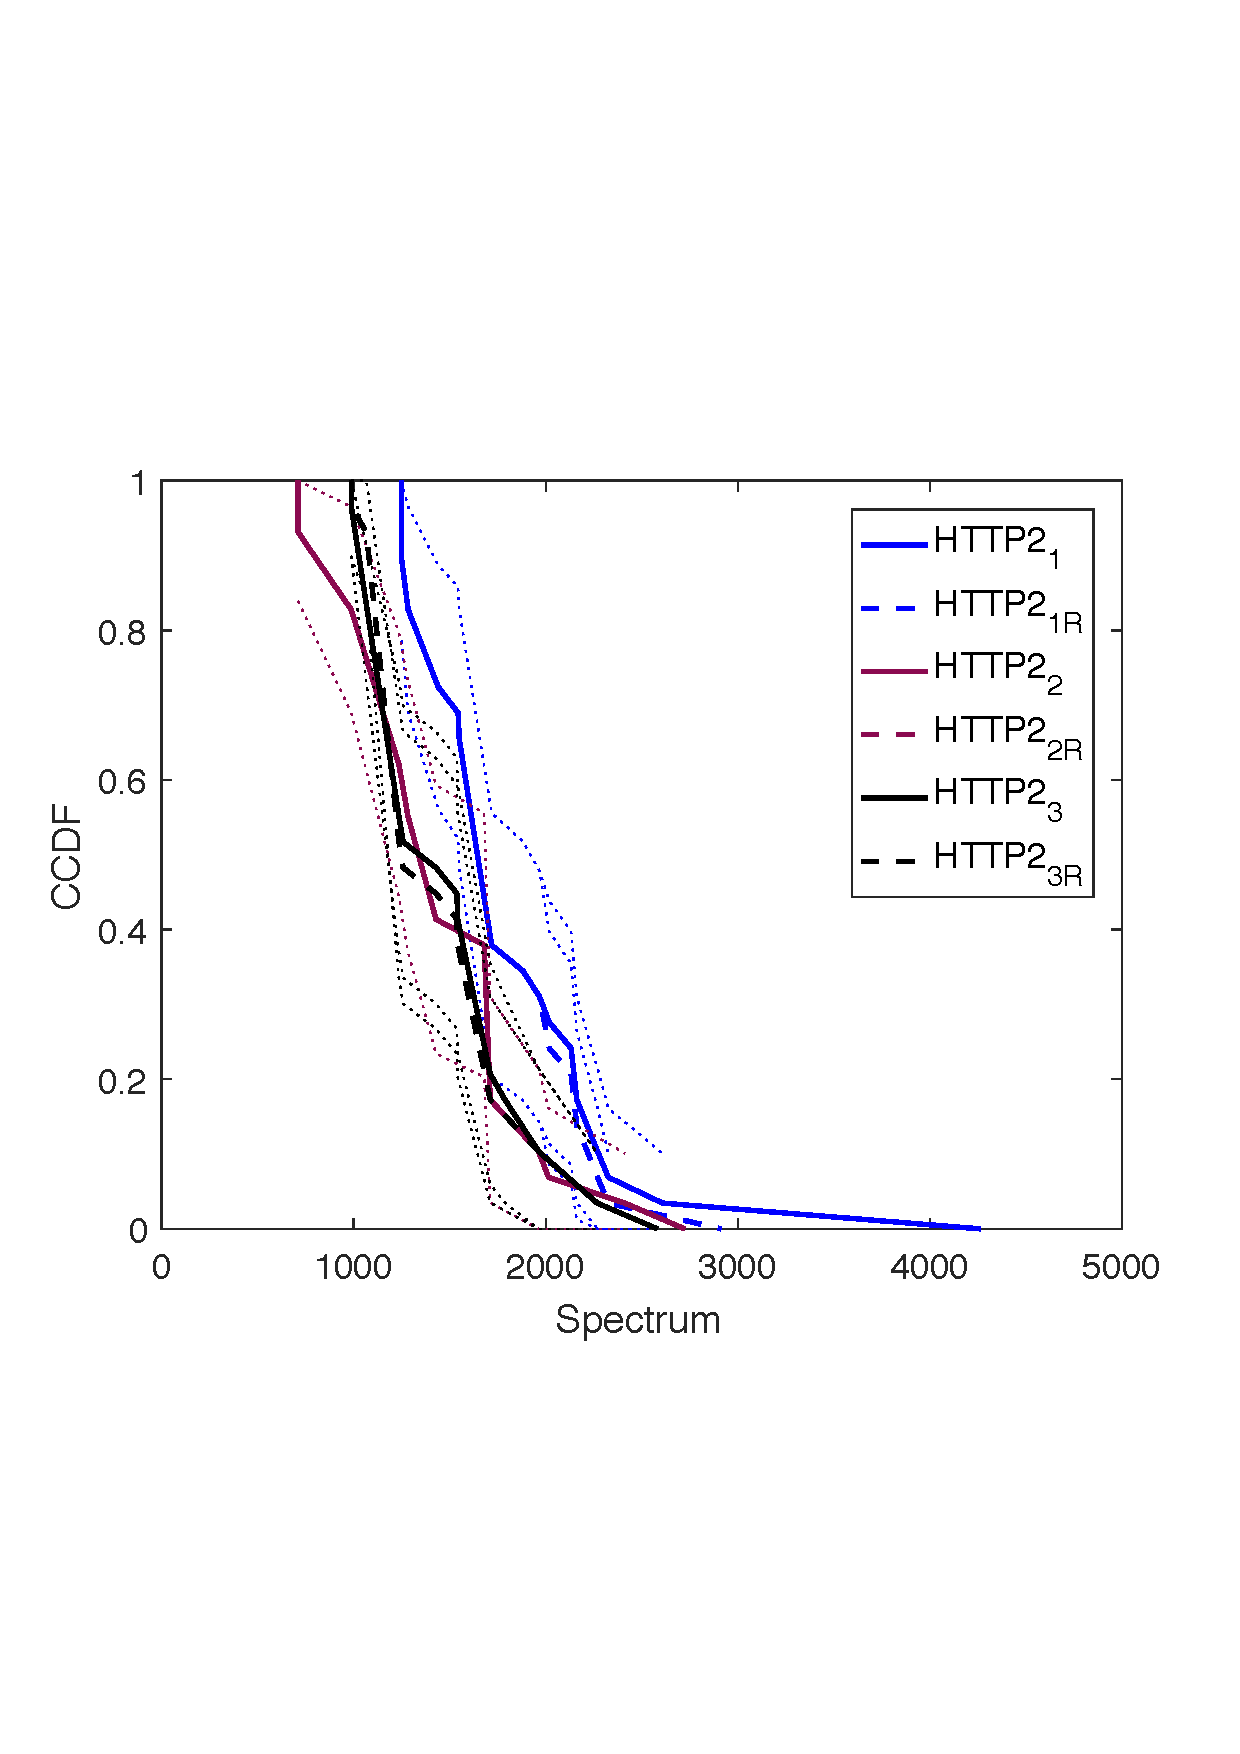
\includegraphics[trim={0 7cm 0 7cm}, scale=0.25]{figures/CDF_magswitch_squad_parallel_http2_nd18.pdf}
    \caption{}
    \label{fig:phttp2magsw}
  \end{subfigure}
 \centering
  \caption{Parallel Client Measurements - Three HTTP2 Clients. All three clients experience comparable QoE and HTTP/HTTP/2 exhibits fairness compared to QUIC. However, the average bitrate is low since HTTP/2 supports multiplexing but continues to be limited by TCP parameters, which leads to conservative behavior.}
  \label{fig:phttp2}
\end {figure*}
\begin{figure*}[t!]
\centering
\begin{subfigure}[t]{0.33\textwidth}
   \captionsetup{justification=centering,margin=4.5cm}
    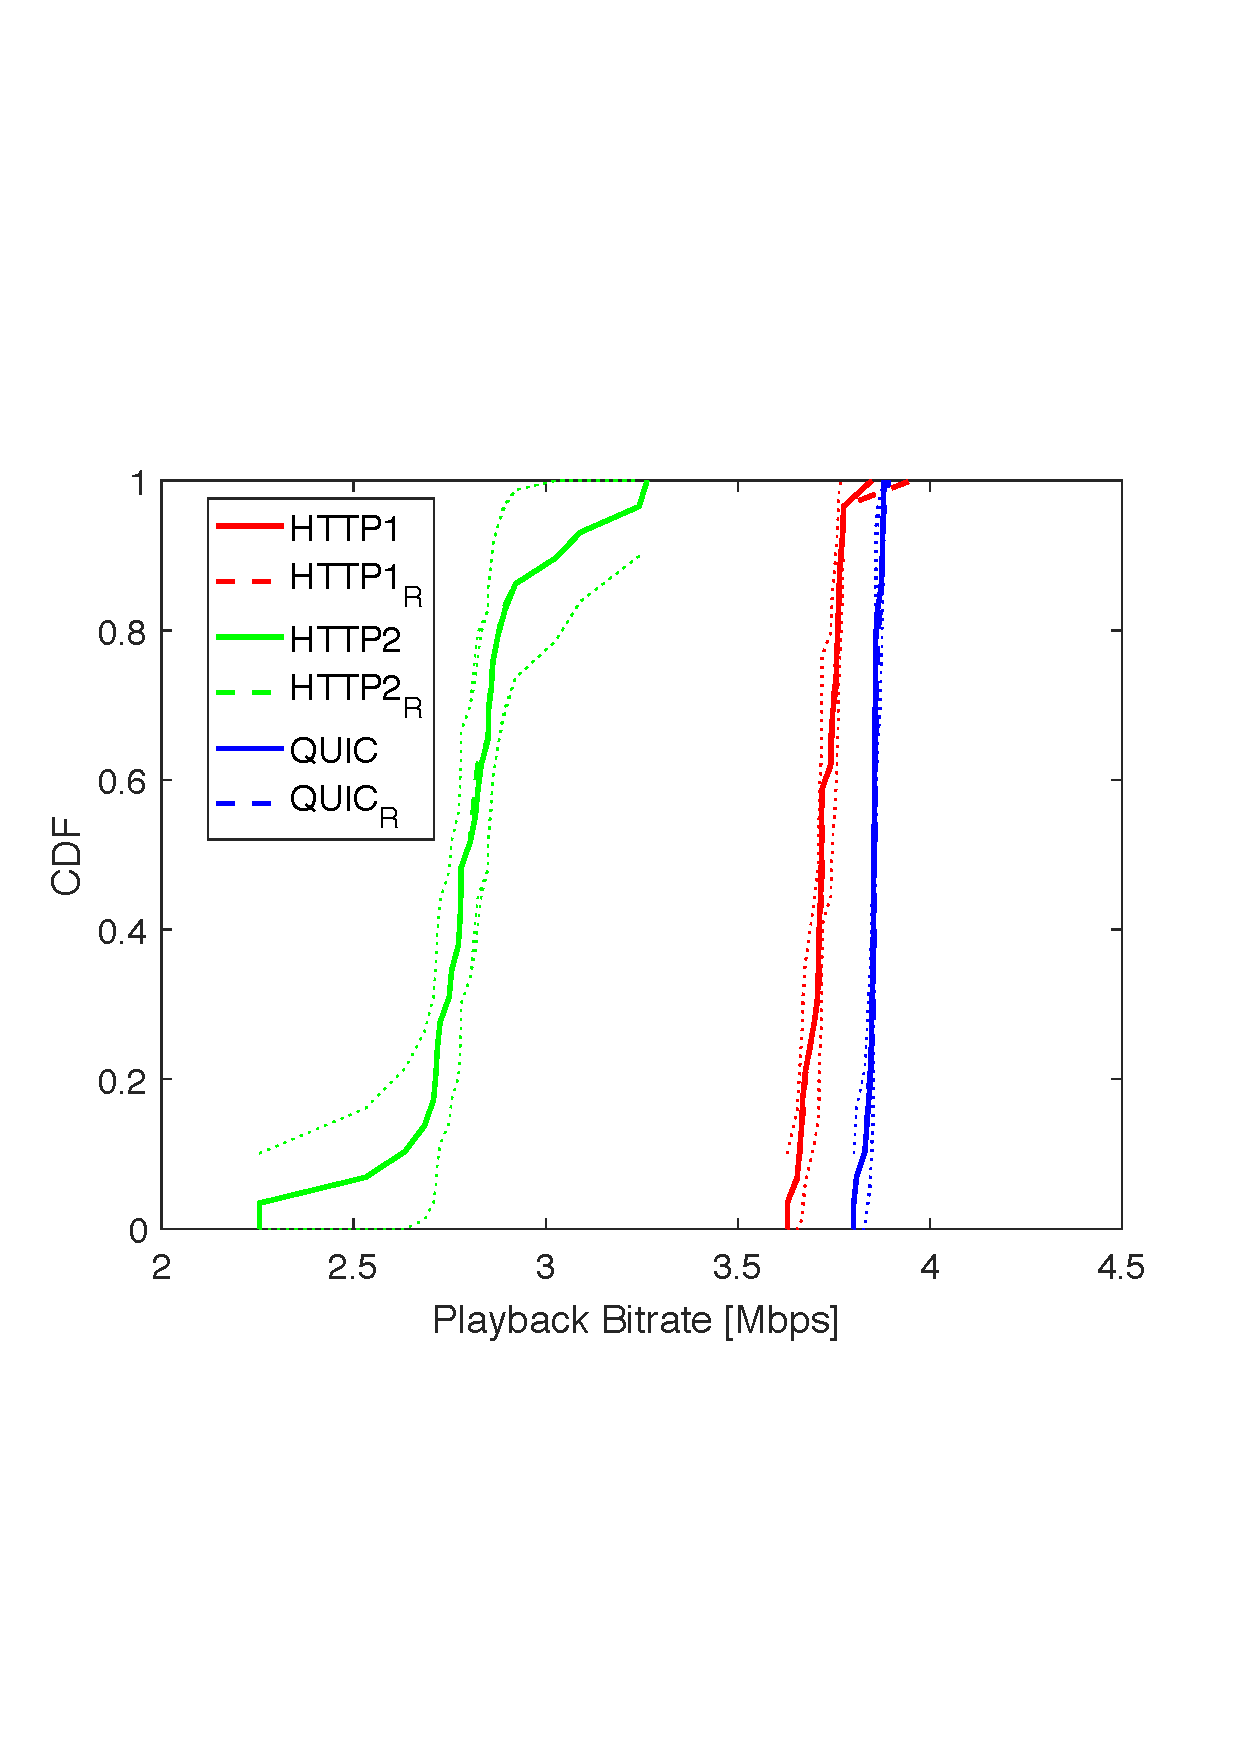
\includegraphics[trim={0 7cm 0 7cm}, scale=0.25]{figures/CDF_bitrat_squad_mixed_clients_nd18.pdf}
     \caption{}
    \label{fig:pmixedbitrate}
  \end{subfigure}
  \begin{subfigure}[t]{0.33\textwidth}
  \captionsetup{justification=raggedright,singlelinecheck=false,margin=2.5cm}
    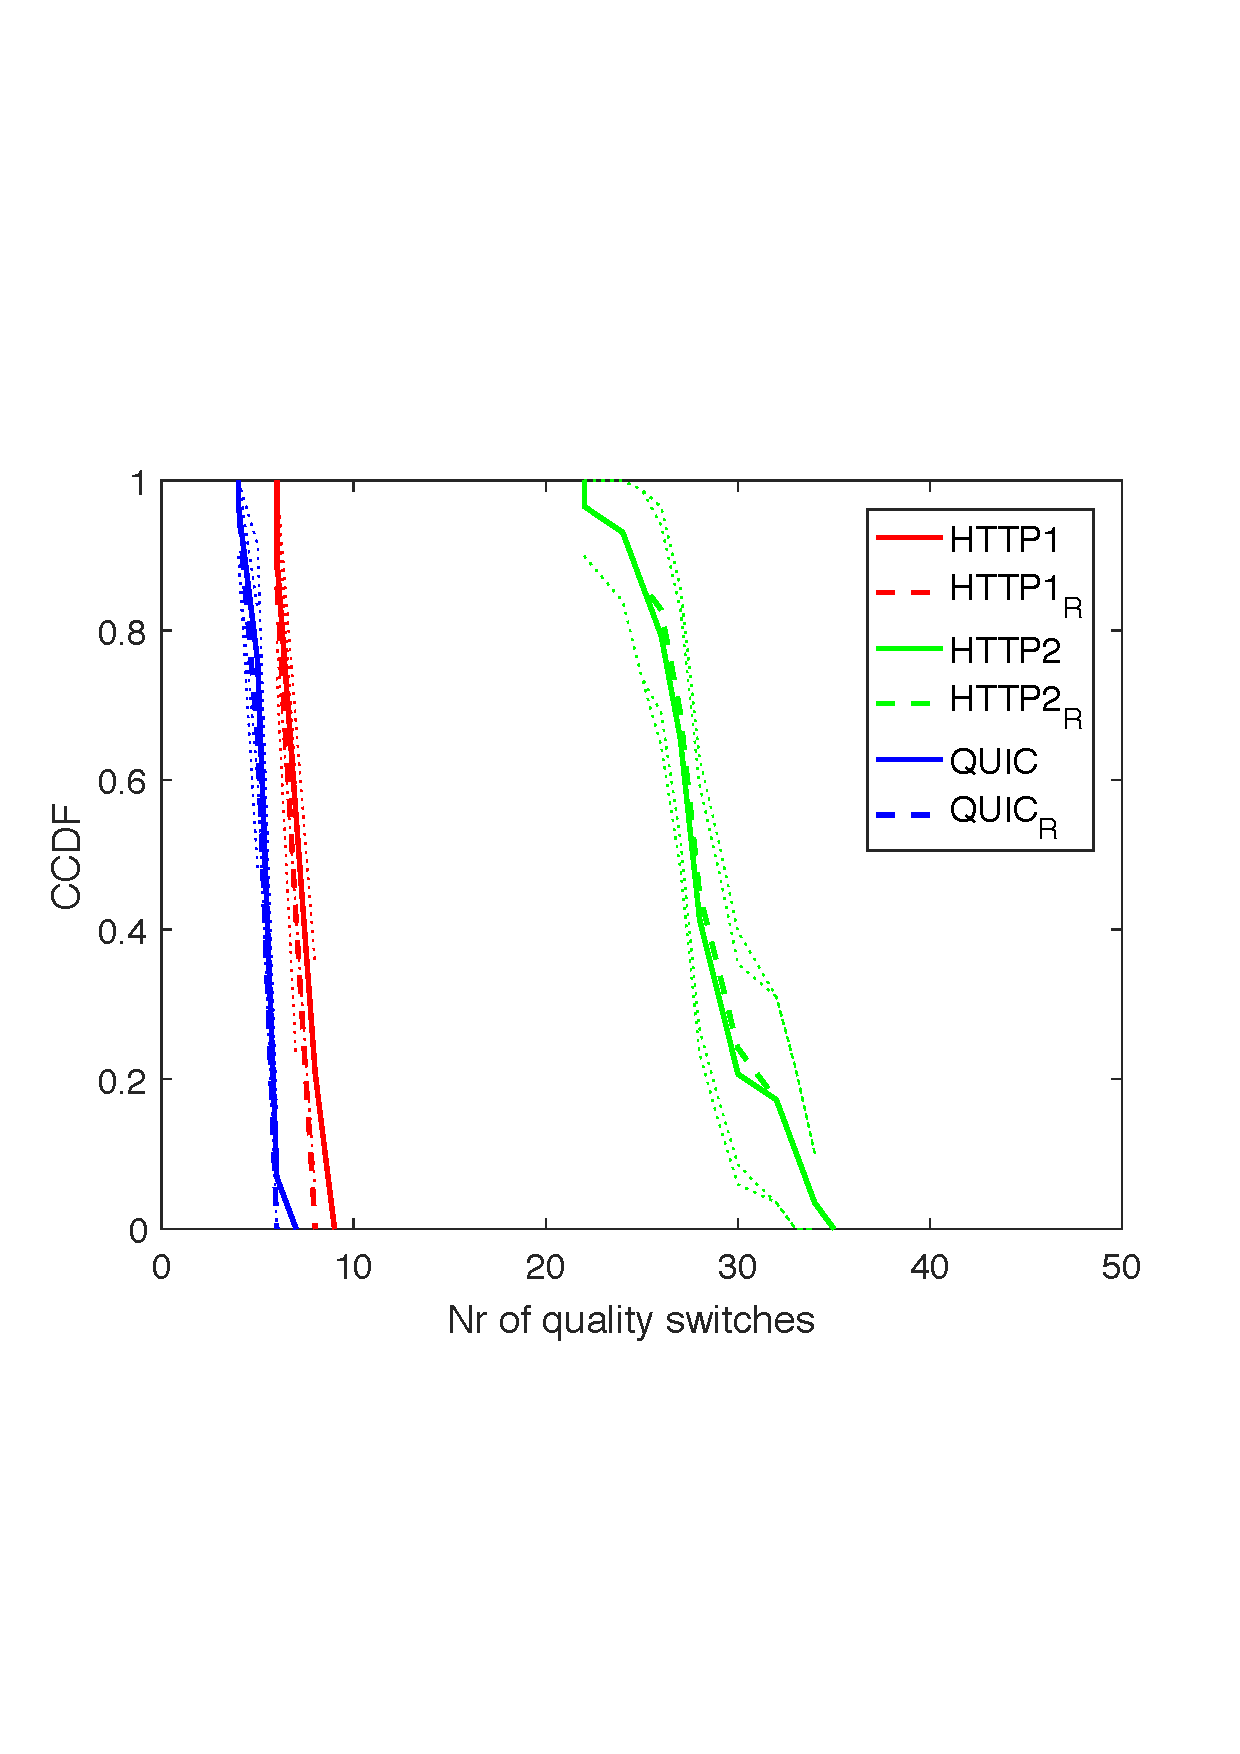
\includegraphics[trim={0 7cm 0 7cm}, scale=0.25]{figures/CDF_cntswitch_squad_mixed_clients_nd18.pdf}
    \caption{}
    \label{fig:pmixedcntsw}
  \end{subfigure}
  \begin{subfigure}[t]{0.33\textwidth}
  \captionsetup{justification=centering,margin=1.5cm}
    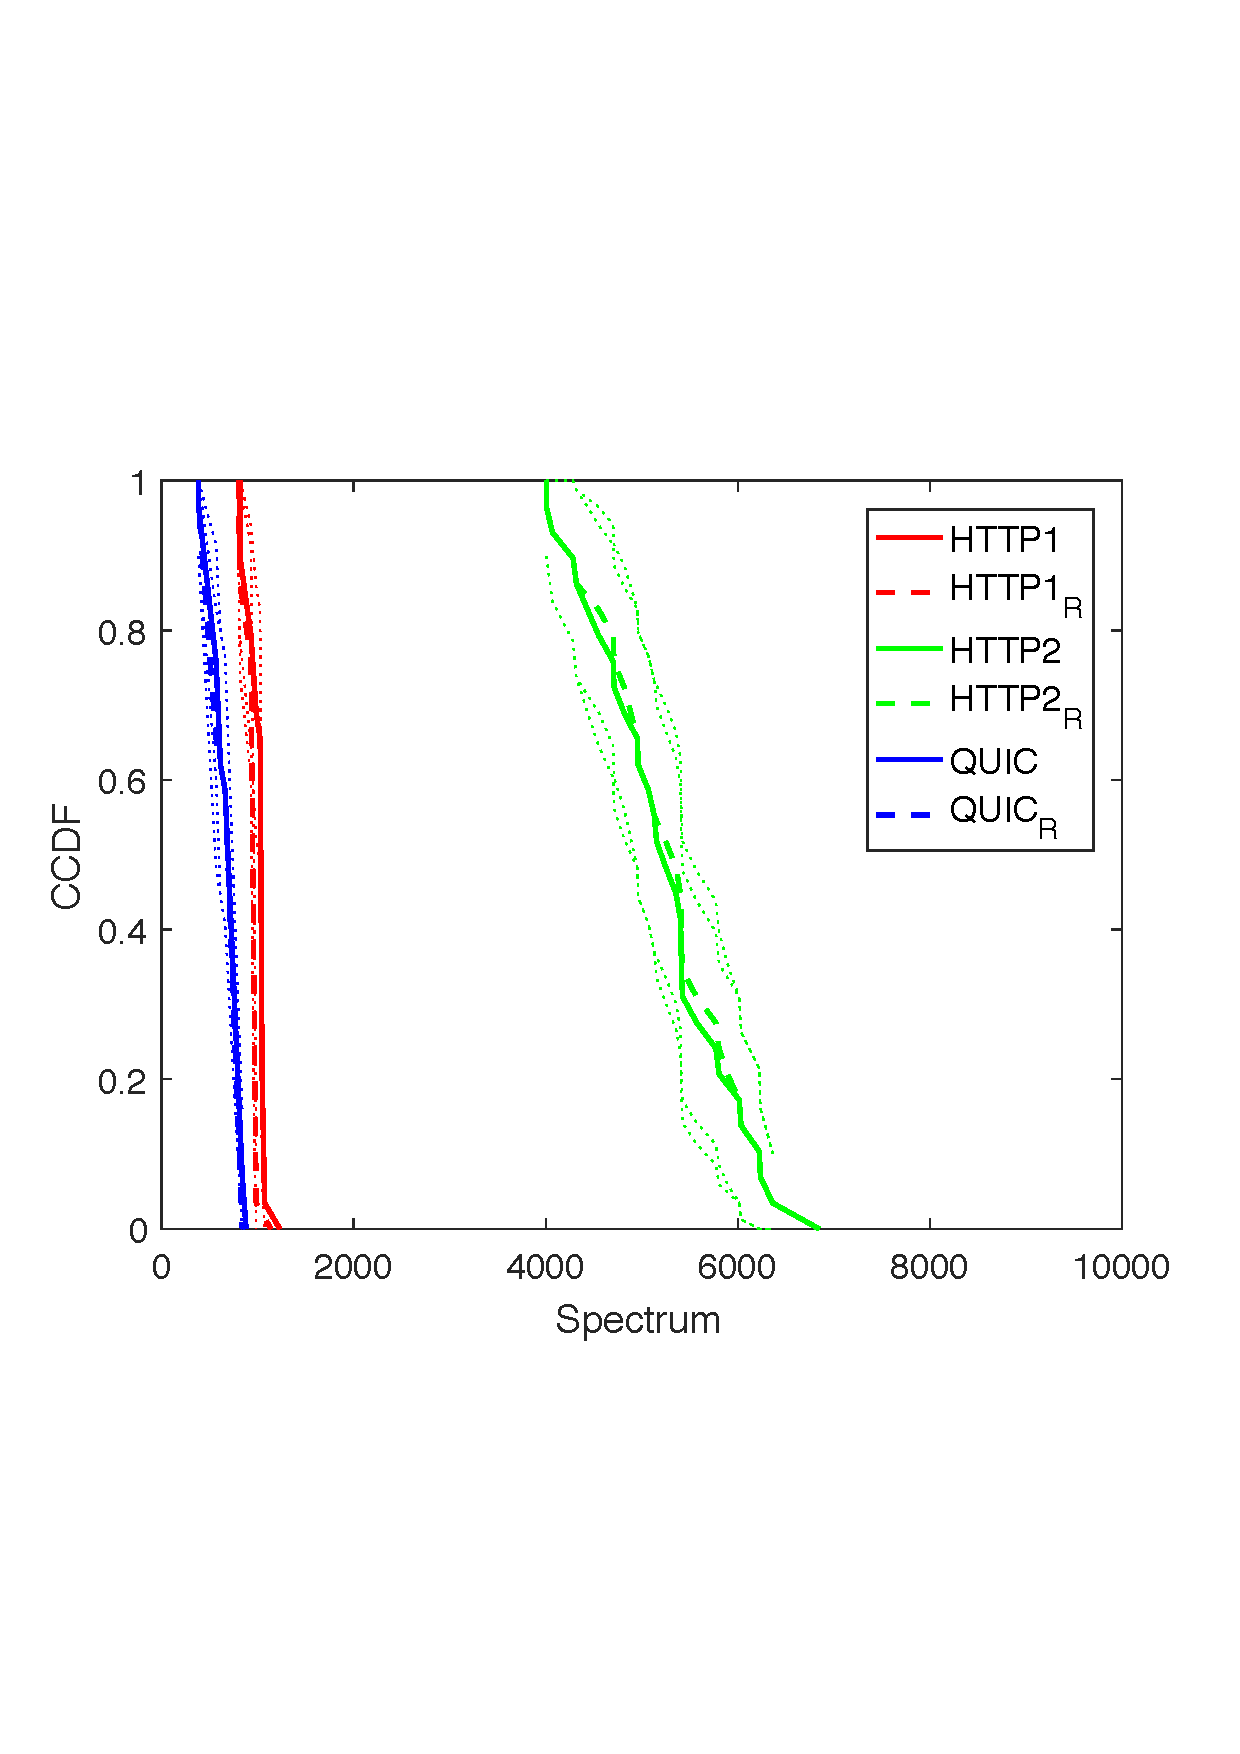
\includegraphics[trim={0 7cm 0 7cm}, scale=0.25]{figures/CDF_magswitch_squad_mixed_clients_nd18.pdf}
    \caption{}
    \label{fig:pmixedmagsw}
  \end{subfigure}
    \begin{subfigure}[t]{0.33\textwidth}
  \captionsetup{justification=raggedright,singlelinecheck=false,margin=2.5cm}
    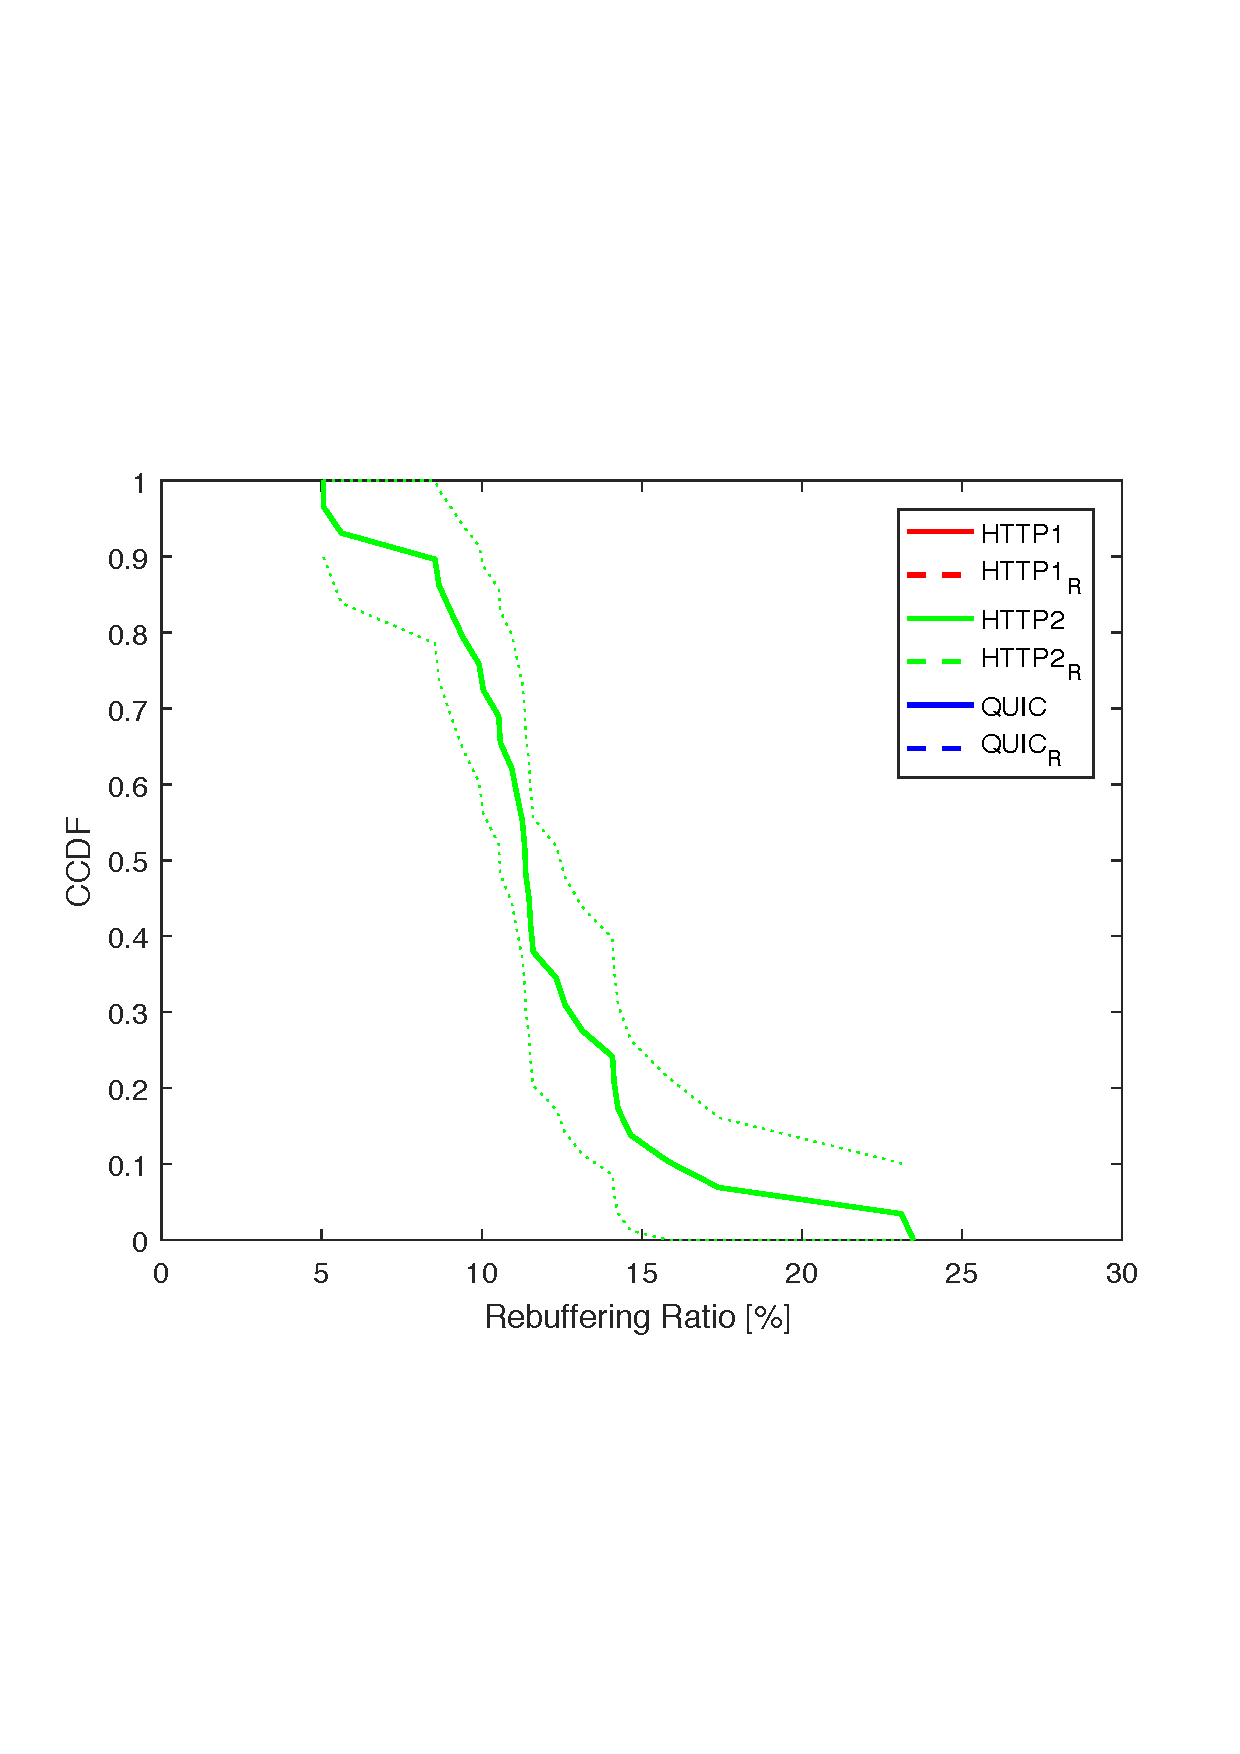
\includegraphics[trim={0 7cm 0 7cm}, scale=0.25]{figures/CDF_rebuffer_squad_mixed_clients_nd18.pdf}
    \caption{}
    \label{fig:pmixedrebuf}
  \end{subfigure}
 \centering
  \caption{Parallel Client Measurements - One HTTP1.1, one HTTP/2 and one QUIC Client. HTTP/2 experiences the worst QoE of all while QUIC clients perform comparatively better than HTTP1.1.}
  \label{fig:pmixed}
\end {figure*}
\fi
\begin{table}[h]
\centering
 \begin{tabular}{ | l | c | c | r | }
    \hline
      & \textit{Client1} & \textit{Client2} & \textit{Client3}\\ \hline \hline
     Average \%Retransmissions & 0.8$\pm$1.3  &1.7$\pm1.3$  &1.0$\pm$0.9  \\
    \hline
  \end{tabular}
  \caption{ABR Segment Retransmissions for three parallel QUIC clients}
           \vspace{-30pt}
    \label{tab:retx_parallel_quic}
    \centering
\end{table}
%with the default Explicit Congestion Notification (ECN) setting, i.e, we enable ECN when requested by incoming connections but do not request ECN on outgoing connections \MZ{[Is %the information about ECN essential for our work or can we take it out?]}. 
\subsection{Internet}
\begin{figure*}[t!]
\centering
\begin{subfigure}[t]{0.33\textwidth}
   \captionsetup{justification=centering,margin=4.5cm}
    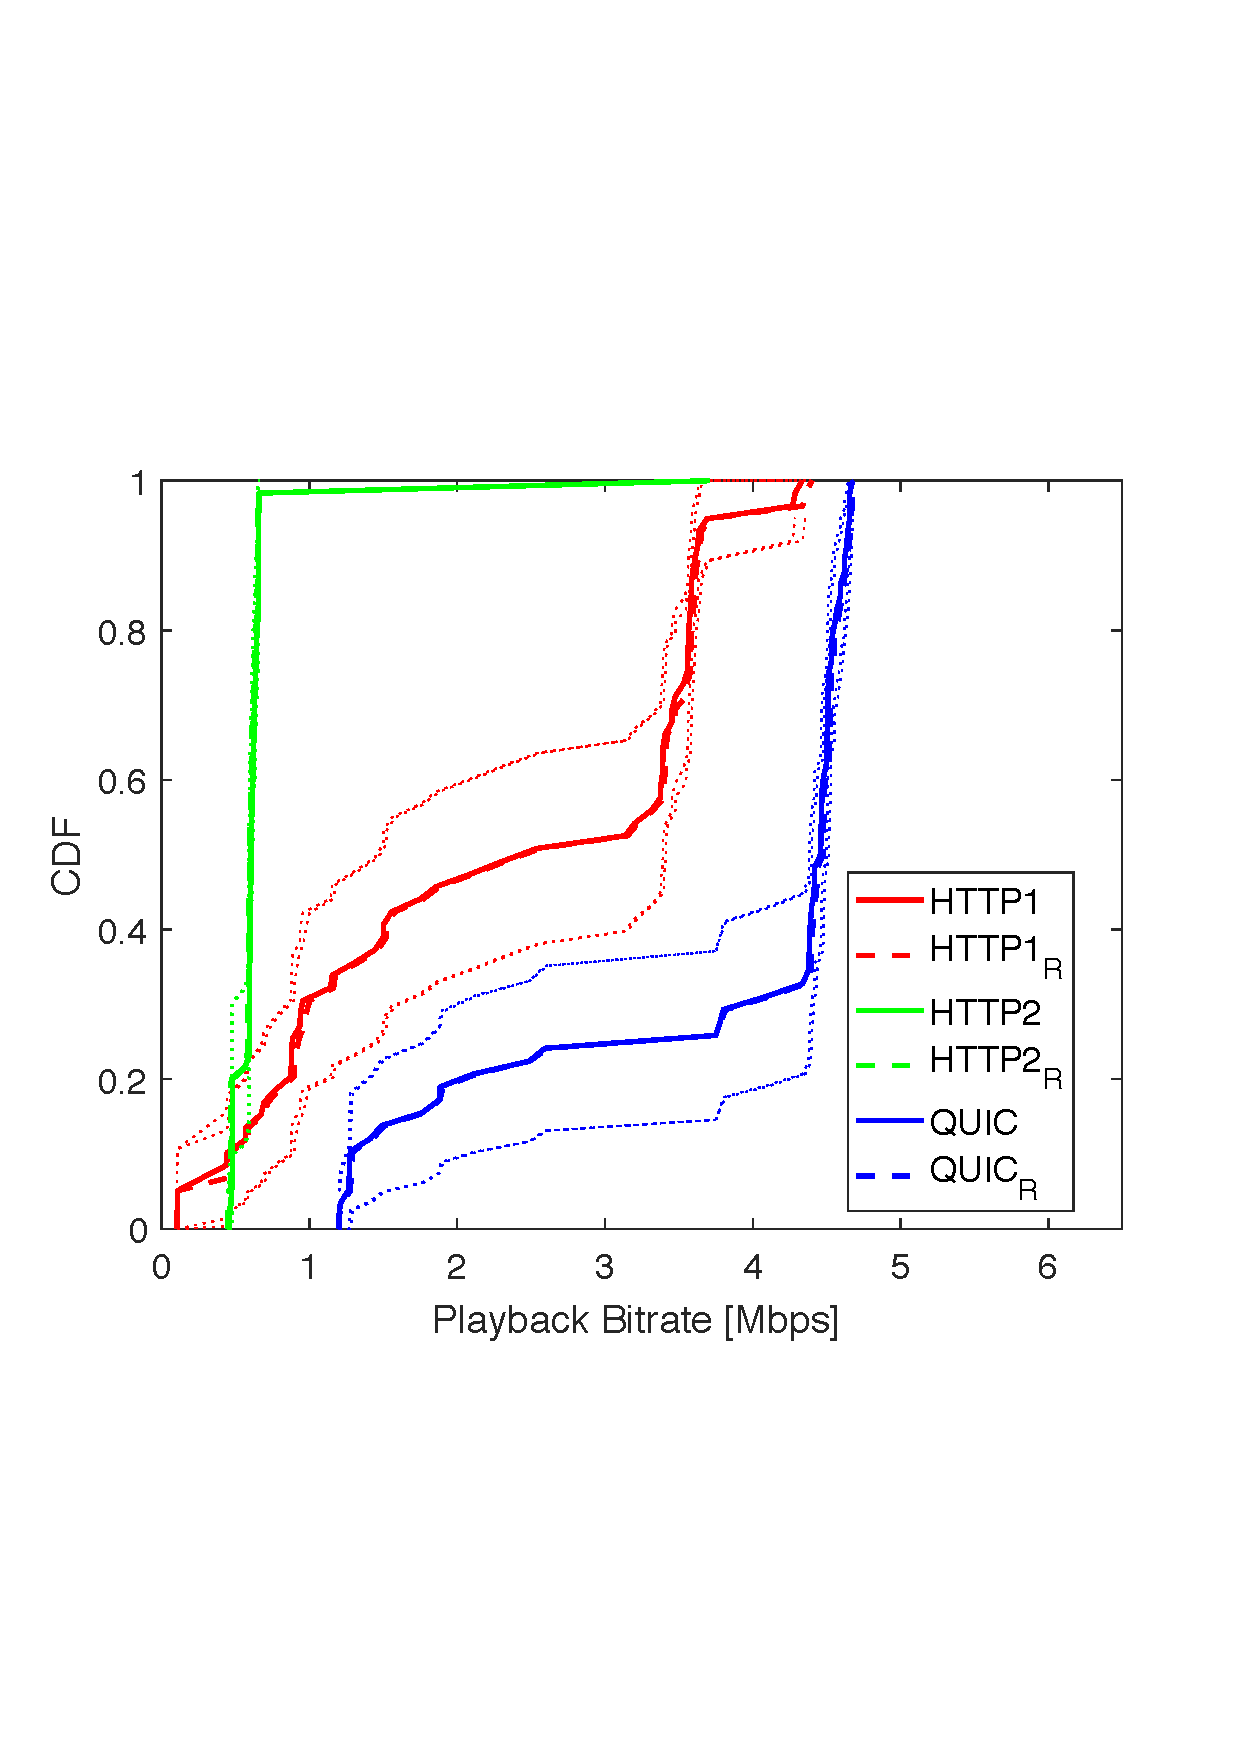
\includegraphics[trim={0 7cm 0 7cm}, scale=0.25]{figures/CDF_bitrat_squad_ec2Mumbai_nd18.pdf}
     \caption{}
    \label{fig:ec2Mumbaibitrate}
  \end{subfigure}
  \begin{subfigure}[t]{0.33\textwidth}
  \captionsetup{justification=raggedright,singlelinecheck=false,margin=2.5cm}
    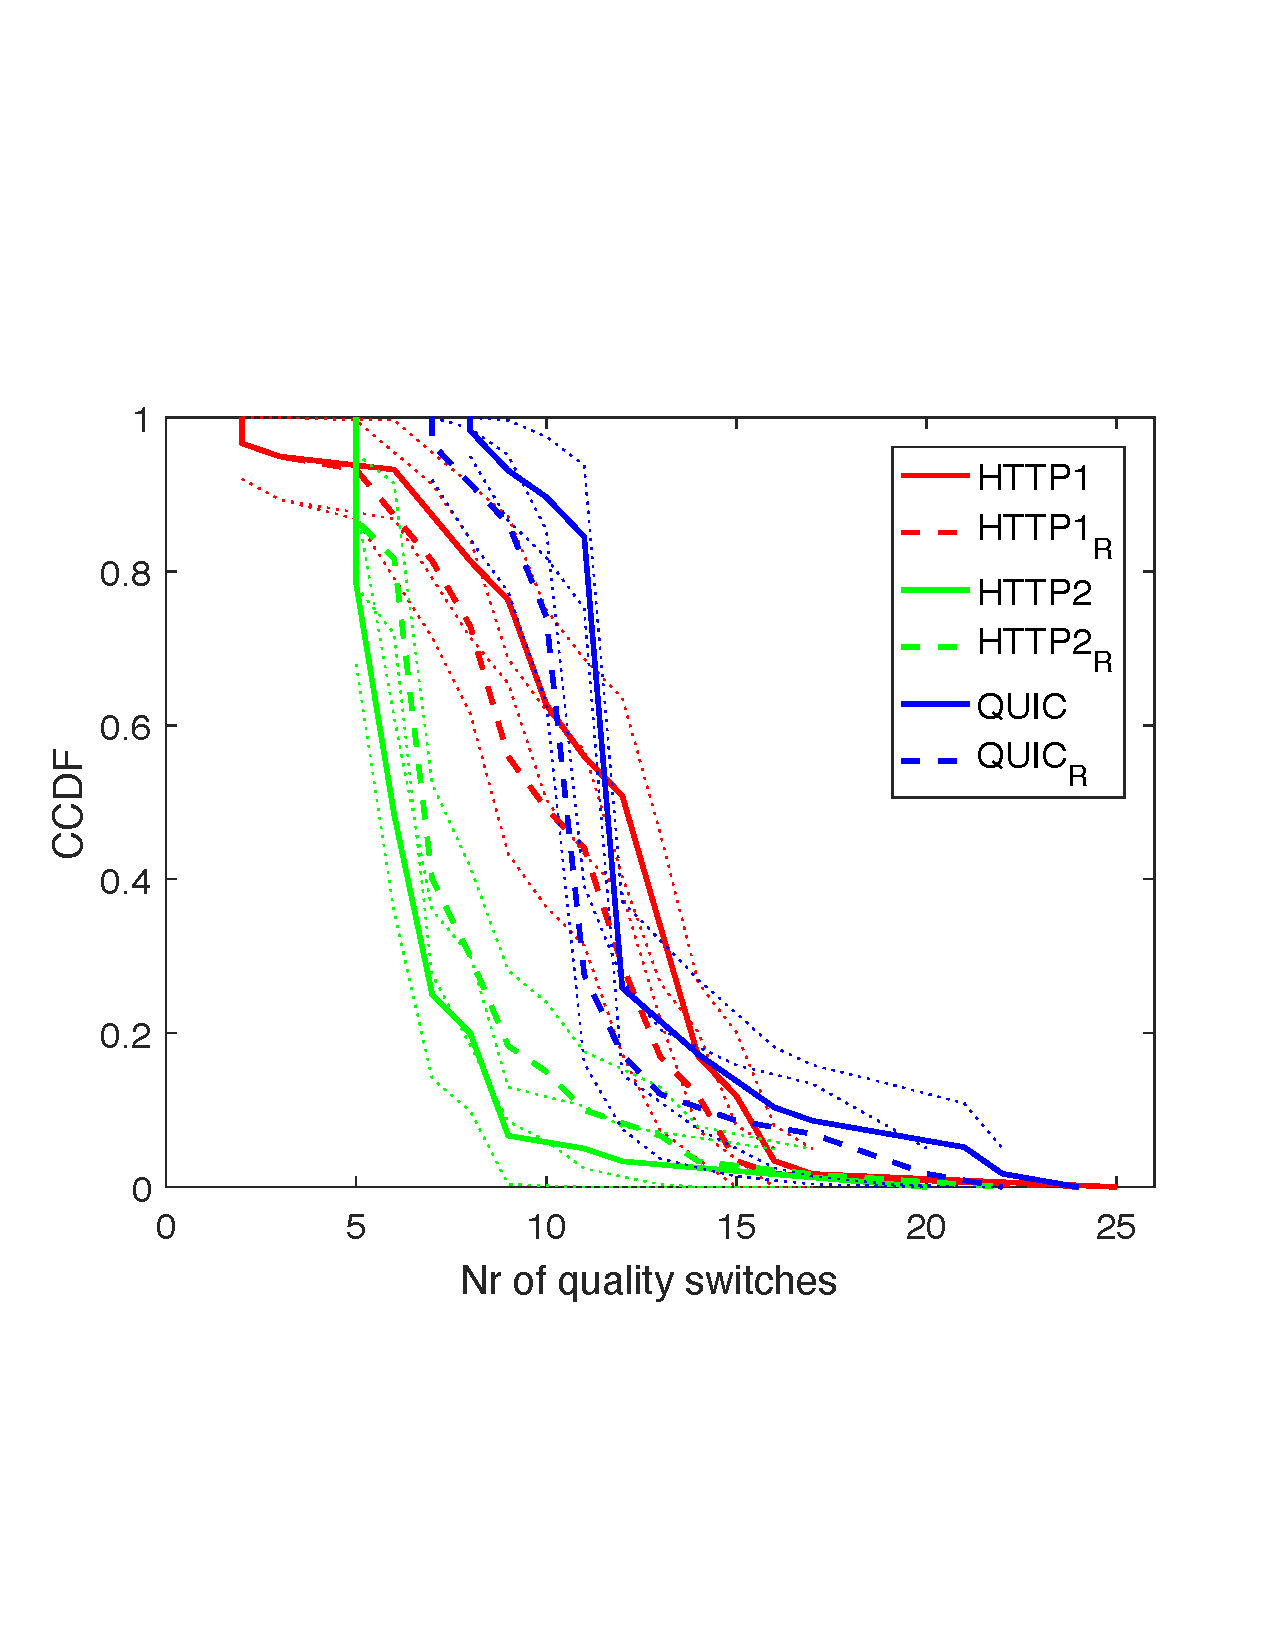
\includegraphics[trim={0 6cm 0 7cm}, scale=0.25]{figures/CDF_cntswitch_squad_ec2Mumbai_nd18.pdf}
    \caption{}
    \label{fig:ec2Mumbaicntswitch}
  \end{subfigure}
  \begin{subfigure}[t]{0.33\textwidth}
  \captionsetup{justification=centering,margin=1.5cm}
    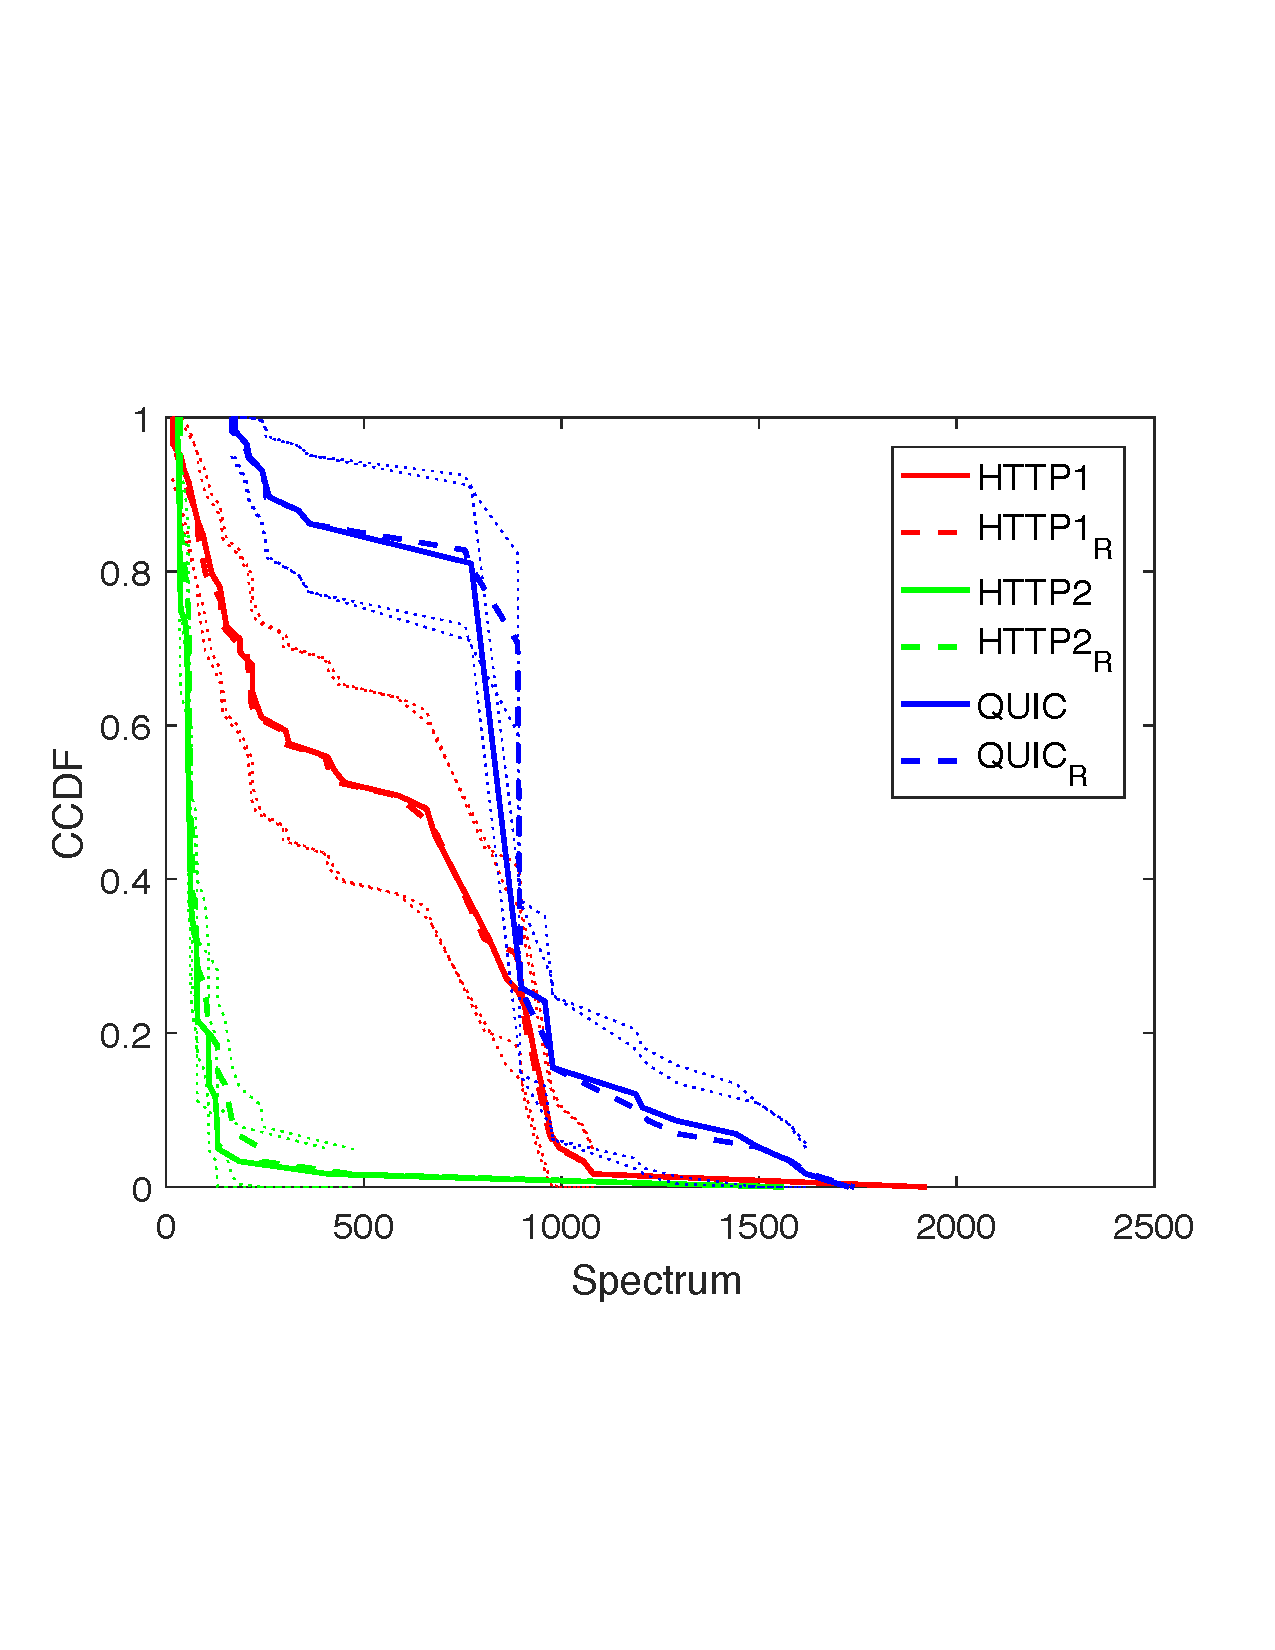
\includegraphics[trim={0 6cm 0 7cm}, scale=0.25]{figures/CDF_magswitch_squad_ec2Mumbai_nd18.pdf}
    \caption{}
    \label{fig:ec2Mumbaimagswitch}
  \end{subfigure}
 \centering
   \vspace{-15pt}
  \caption{Internet Measurements - ABR streaming is performed over inter-continental links with the server at Amazon EC2 in India and the client on the US East Coast. QUIC far outperforms HTTP/1.1 and HTTP/2 in terms of QoE, i.e., provides significant improvement in Average Quality Bitrate while providing comparable reduction in the number of quality switches.}
  \label{fig:ec2Mumbai}
  \vspace{-10pt}
\end {figure*}
For the Internet measurements, we use Amazon EC2 virtual machines in Mumbai, India and Oregon, USA as servers and a client in the UMass Amherst campus network to perform inter-continental and intra-continental measurements, respectively. Here, we repeat each experiment 60 times to account for increased network variations in an uncontrolled environment. Since the bottleneck bandwidth during off-peak hours can be high, we use a different video dataset with higher qualities, \texttt{RedBull} \cite{lederer2012dynamic}, and modify the MPD to contain the following bitrates $\{${0.10, 0.15, 0.20, 0.25, 0.30, 0.40, 0.50, 0.70, 
0.90, 1.20, 1.50, 2.00, 2.50, 3.00, 4.00, 5.00, 6.00}$\}$Mbps for a video duration of 300s and a segment duration of 2s.
Figure \ref{fig:ec2Mumbai} presents results for measurements "in the wild" over inter-continental links from an EC2 web server located in India. The average quality bitrate (in Fig. \ref{fig:ec2Mumbaibitrate}) is significantly higher for QUIC than HTTP/2 and HTTP/1.1. Fig. \ref{fig:ec2Mumbaicntswitch} shows that $\#QS$ is also reduced with the use of QUIC and HTTP/1.1 retransmissions indicating an overall high QoE. Table \ref{tab:qoe_abr_internet} shows QoE metrics for similar measurements conducted with the server located at EC2 in Oregon. Here, it is worth mentioning that all QoE metrics are comparable for HTTP/1.1 and QUIC where QUIC is marginally better than HTTP/1.1, but are significantly improved over HTTP/2 (for example, the average bitrate $AQB$ is less than half of that obtained with HTTP/1.1 and QUIC). Since Internet traffic is predominantly comprised of TCP flows, these results further reinforce the observations made in Sect. \ref{subsubsec:hol} for high delay, high loss paths with competing TCP traffic. Our results show that the use of QUIC results in better QoE in the case of inter-continental as well as intra-continental links, while the advantage compared to HTTP/1.1 is more significant in case of the former.

\begin{comment}
\begin{table*}[h]
\centering
 \begin{tabular}{ | l | c | c | c | c | c | c | r | }
    \hline
      & $AQB$ (Mbps) &  $AQB_{R}$ (Mbps) & $\#QS$ & $\#QS_{R}$ & $H$ & $H_{R}$ & $RB_{R}$(\%)\\ \hline \hline
     %Single Clients: UDP-W (8M-5M) & 3.90$\pm0.1$ & 3.93$\pm$0.1  & 8.7$\pm$0.9 & 6.1$\pm$1.6 & 1596$\pm$204 & 919$\pm$306 & 0   \\ \hline
     Parallel Clients: HTTP/1.1 &  &  &  &  &  &  &  \\ \hline
     Parallel Clients: HTTP/2 & 3.13$\pm$0.2 & 3.14$\pm$0.2  & 9.58$\pm$2.0 & 9.45$\pm$1.7 & 1616$\pm$499 & 1587$\pm$428 & 0 \\ 
    \hline
  \end{tabular}
  \caption{ABR Quality of Experience: Parallel Clients}
    \label{tab:qoe_abr_ctrl}
    \centering
\end{table*}
\end{comment}
\begin{table*}[h]
\centering
 \begin{tabular}{ | l | c | c | c | c | c | c | r | }
    \hline
      & $AQB$ (Mbps) &  $AQB_{R}$ (Mbps) & $\#QS$ & $\#QS_{R}$ & $H$ & $H_{R}$ & $RB_{R}$(\%)\\ \hline \hline
     Internet: HTTP/1.1 & 5.31$\pm$0.1 & 5.66$\pm$0.1  & 8.48$\pm$1.4 & 3.82$\pm$2.1 & 490$\pm$213 & 242$\pm$312 & 0 \\ \hline
     Internet: HTTP/2 & 2.12$\pm$0.6 & 2.13$\pm$0.6  & 9.09$\pm$2.6 & 6.98$\pm$2.5 & 552$\pm$280 & 447$\pm$255  & 0$\pm$10.8\\ \hline
     Internet: QUIC & 5.31$\pm$1.9 & 5.44$\pm$0.2  & 7.91$\pm$1.8 & 5.81$\pm$1.7 & 445$\pm$299 & 351$\pm$273  & 0\\
    \hline
  \end{tabular}
  \caption{ABR Quality of Experience over the Internet: Amazon EC2 Oregon - US East Coast}
  \vspace{-20pt}
    \label{tab:qoe_abr_internet}
    \centering
\end{table*}
%\section{Discussion}
\label{sec:dicsussion}

\subsection{Multipath}
\label{sec:mpath}
Especially in the case of mobile devices like smart phones the Internet can be accessed via different technologies (e.g., WiFi and LTE). Thus, videos can be streamed via multipath to such a device, which has been suggested for ABR streaming~\cite{Han:CoNEXT:2016}. While we do not investigate the potential impact of multipath streaming based on HTTP/2 in this paper, we briefly outline the potential benefits of its usage. First, a multipath approach can increase the available bandwidth between client and server and, accordingly result in a higher quality streaming session. Second, it can be decided what data is sent on which path. Third, even if the connection to one of the access technologies is lost streaming can be continued. Though, potentially in a lower quality.

Since the retransmission approach we present in this paper is already based on the concept of separate streams in an HTTP/2 session, making use of a multipath approach is a logical consequence. For example, one could envision a scenario in which original segments are transmitted over the WiFi path, while retransmission are scheduled on the stream that uses the LTE path. While a TCP-based approach will still have the drawback of HOL blocking (as described in Sect.~\ref{subsec:example}), we conjecture that a QUIC-based multipath approach will perform better.

\subsection{SDN Support}
\label{subsec:sdn}
In our work on network assisted ABR streaming~\cite{Bhat:MMSys:2017}, we have shown how link bandwidth information with increased accuracy can improve the QoE of a streaming session. Such information can also be beneficial for the retransmission approach we present in this paper. In~\cite{Bhat:MMSys:2017}, we have shown that a combination of information on past link bandwidth and an ARIMA-based prediction of future link bandwidth can assist the bitrate quality selection of DASH streaming algorithms. In the case of our segment retransmission approach, ARIMA-based bandwidth predictions can be taken into account to decide if a segment can be retransmitted in time before its playout deadline.
\section{Related Work}
\label{sec:relatedwork}
%Recent works that evaluate alternative transport protocols for adaptive bitrate (ABR) video streaming include the work by McQuistin et al. \cite{McQuistin}. The authors present \textit{TCP Hollywood}, a TCP variant, which implements out-of-order delivery and inconsistent retransmissions in order to improve good-put of video streaming applications. 
A recent paper by Google \cite{Langley:SIGCOMM:2017} provides a detailed analysis of an Internet-scale deployment of QUIC. They specifically look at latency and rebuffer rate in order to understand the performance implications of QUIC for video streaming over YouTube. Timmerer et al. \cite{timmerer2016advanced} evaluate ABR streaming over QUIC for varying network latencies and show that there is no significant benefit to QoE streaming with the use of QUIC. In \cite{szaboquic}, a demonstration by Szab\'o et al. provides a new congestion control mechanism for QUIC that aggressively varies download rate according to a buffer-based priority level assigned by the ABR streaming client.
Carlucci et al. \cite{Carlucci:2015} present results that compare TCP and QUIC under varying network conditions and buffer size. In~\cite{Kakhki:IMC:2017}, Kakhki et al. perform a detailed analysis of QUIC under varying network conditions to investigate the benefits of using QUIC for applications such as web browsing and video streaming over YouTube. The authors of \cite{AYAD201890} also compare the performance of several rate adaptive DASH players including QUIC and conclude that QUIC is more aggressive compared to TCP. The authors of \cite{BHayes} devise and deploy an SDN approach to to improve the QoE of ABR streaming by monitoring MPTCP retransmissions where their system dynamically switches between network paths and protocols to mitigate re-ordering effects. While we similarly compare the performance of TCP (using HTTP/1.1 and HTTP/2) with QUIC, our work is more focussed on the potential benefits that QUIC can provide for video streaming especially with respect to retransmitting video segments in higher qualities. Similar experiments are performed by the authors of \cite{huysegems2015http}, where they use the multiplexing feature of HTTP/2 to simultaneously request multiple qualities of a segment. While retransmissions can be regarded as an additional burden on the available bandwidth we note that recent works such as~\cite{Vulimiri:CoNext} suggest different types of redundant transmission to provide higher QoS. In contrast to~\cite{huysegems2015http} and~\cite{Vulimiri:CoNext}, we only invoke retransmissions in a systematic way, thereby guaranteeing an improvement in QoE while also minimizing the consumption of additional bandwidth. Moreover, in order to analyze the implications of specific network conditions that affect ABR video streaming, we design, develop and prototype such a system in a nearly isolated, controlled testbed environment.

Legacy protocols that perform adaptive bitrate video streaming over UDP include systems such as Real-time Transport Protocol (RTP) \cite{rtp} and Stream Control Transport Protocol (SCTP) \cite{sctp}. Similar to QUIC, SCTP also allows multiplexing of multiple chunks into one packet and avoids HOL blocking, thus, allowing unordered delivery to the application layer. Unlike QUIC, SCTP implements 
congestion control according to the TCP \textit{NewReno} specification which uses Selective Acknowledgement (SACK) for loss recovery.
% the \textit{NewReno} form of TCP congestion control including TCP's method of Selective Acknowledgement (SACK) for loss recovery. 
Another example of an ABR protocol over UDP is the Video Transport Protocol (VTP) which was designed and evaluated by Balk et al. \cite{balk2003adaptive}. In this work, the authors employ a form of congestion avoidance where the sending rate at the server is increased by a single packet for every RTT measurement. This design is different from the AIMD congestion control employed by TCP and QUIC since it eliminates the effect of slow start and attempts to provide an accurate estimate of the available bandwidth in the network. Some drawbacks of this approach are the requirement of two UDP sockets for every connection and the use of Berkeley Packet Filters to collect timestamps at the server and client for every video stream, thus, reducing both performance and scalability of the system. Although there are a number of server push approaches such as \cite{huysegems2015http} and \cite{xiao2016evaluating} that have been proposed for HTTP/2, adapting such systems for retransmissions would not scale since the computation and storage overhead incurred on the server per individual client connection would render such an approach infeasible.
\begin{comment}
MORE RELATED WORK:

HotNets 2017~\cite{Narayan:HotNets:2017} \DB{This is only remotely related as it looks at software defined congestion control}

Sigcomm 2017 Carousel~\cite{Saeed:Sigcomm:2017} \DB{Remotely related as they look at timing wheels and rate control}
\end{comment}

\section{Conclusion}
In this work, we conduct systematic experiments to analyze the performance implications of various HTTP/2 transport layer candidates on ABR streaming systems, particularly with respect to ABR segment retransmissions. We leverage the multiplexing feature of QUIC and HTTP/2 in order to efficiently implement parallel retransmissions in a higher quality with the objective of maximizing average quality bitrate while also minimizing bitrate variations throughout the duration of a streaming session. We use a nearly isolated testbed setup in CloudLab and measurements "in the wild" to show that QUIC retransmissions provide a significantly better QoE than TCP in high latency, high loss networks while exhibiting comparable QoE in low latency, low loss networks.
\label{sec:conc}

\clearpage
%\bibliography{sigproc}
\bibliographystyle{abbrv}
\balance\bibliography{paperms}  % sigproc.bib is the name of the Bibliography in this case
% You must have a proper ".bib" file
%  and remember to run:
% latex bibtex latex latex
% to resolve all references
%

\end{document}


